% ================================== %
%           Setup document           %
% ================================== %
\documentclass[	a4paper,		%
				12pt,			%
				titlepage,		%
				twoside,		%
				DIV				= 14,			%
				BCOR			= 6mm,			%
				parskip			= half,			%
				numbers 		= noenddot, 	%
				headings 		= small,		%
				cleardoublepage = empty]{scrbook}


% ================================== %
%          Import packages           %
% ================================== %
\usepackage{ae}               	% almost european, virtueller T1-Font
\usepackage{array}          	% fuer aufwändigere Tabellen
\usepackage{colortbl}       	% farbige Tabellen (v. D. Carlisle)
\usepackage{longtable}      	% seitenübergreifende Tabellen
%\usepackage{ltablex}			% Kombiniert longtable mit tabularx
\usepackage{tabularx} 			% automatische Spaltenbreite
			\renewcommand{\arraystretch}{1.3}
\usepackage{color}    			% Farbiger/grauer Text
\usepackage[utf8]{inputenc}
\usepackage[british,ngerman]{babel}
\usepackage{amsfonts}
\usepackage{amsmath}
\usepackage{amssymb}
\usepackage[sc]{mathpazo}	% Palatino Schrift
			\linespread{1.05}
\usepackage[T1]{fontenc}
\renewcommand*\familydefault{\rmdefault}
\usepackage{pdfpages}
\usepackage[T1,hyphens]{url} 	% much like \verb allow line breaks for paths and URLs
\usepackage{calc}
\usepackage[absolute]{textpos} 
\usepackage{ifthen}     \usepackage{lscape}     \usepackage[cmyk,dvipsnames]{xcolor}
\usepackage{setspace}   \usepackage{graphicx}   \usepackage{graphicx,import}
\usepackage{subcaption} \usepackage{svg}		\usepackage[section]{placeins}
\usepackage{tocbasic}   \usepackage{paralist}   \usepackage{amsmath}
\usepackage{booktabs}   \usepackage{multirow}   \usepackage{multicol}
\usepackage{rotating}   \usepackage{mathtools}  \usepackage{mdwlist}
\usepackage{anysize}    \usepackage{pslatex}    \usepackage{wrapfig}
\usepackage{scrhack}    \usepackage{csquotes}   \usepackage{xkeyval}
\usepackage{xfor}       \usepackage{amsgen}     \usepackage{xfrac}
\usepackage{enumitem}

\allowdisplaybreaks[1]
\usepackage{tikz}				% fuer Grafiken, Baeume und Graphen
	\usetikzlibrary{decorations.pathmorphing}
	\usetikzlibrary{shapes}
	\usetikzlibrary{backgrounds} 

%\usepackage{subfig}	 % da Package mit subcaption zusammen nicht funktioniert			

\usepackage[format		= hang,	%
 			margin		= 10pt,	%
 			font		= small]%
 			{caption}			% captions (Bildunterschriften) formatieren
	\captionsetup[figure]{		%
	  		name 		= Figure} %
\usepackage{epstopdf} 			% Konvertiert eps zu pdf, wenn erkannt
\usepackage{fixmath}  			% 
\usepackage{dcolumn}  			% Ausrichtung an Komma oder Punkt
\usepackage{cancel}
\usepackage[
			   bottom,     		% Footnotes appear always on bottom. This is necessary
			               		% especially when floats are used
			   stable,      	% Make footnotes stable in section titles
			   perpage,     	% Reset on each page
			   %para,       	% Place footnotes side by side of in one paragraph.
			   %side,       	% Place footnotes in the margin
			   %ragged,      	% Use RaggedRight
			   %norule,   	  	% suppress rule above footnotes
			   multiple,  	  	% rearrange multiple footnotes intelligent in the text.
			   %symbol,     	% use symbols instead of numbers
			]{footmisc}
\usepackage{varioref} 			% Intelligente Querverweise


% ================================== %
%              Options               %
% ================================== %
%% PDF Settings
\usepackage{hyperref}
\hypersetup{pdfpagelayout 		= {TwoColumnLeft},		
			pdftitle 			= {MA-Nummer-Jahr-ilb},	
			pdfsubject 			= {Arbeitstitel-Kurzform},
			pdfcreator 			= {PDFLaTeX},			
			pdfauthor 			= {Name Matrikelnummer},
			plainpages 			= false,				
			linkcolor 			= blue,					
			citecolor 			= purple,				
			filecolor 			= green,				
			urlcolor 			= blue,					
			pdfborder 			= {0 0 0.5},			
			raiselinks 			= true,					
		    bookmarksopenlevel	= 1,					
			bookmarksopen		= true,					
		    bookmarksnumbered	= true,					
			colorlinks 			= true,					
			draft 				= false}	
            
%% Footers and headers
\usepackage[automark,markcase=ignoreuppdercase,headsepline]{scrlayer-scrpage}
\clearpairofpagestyles
\setkomafont{pageheadfoot}{\normalfont\normalcolor}
\setkomafont{pagenumber}{\normalfont}
\automark[section]{chapter}		% scrheadings mit Kapitel bzw. section und Seitenzahl oben
\ofoot[]{}                      % scrplain ohne alles
\KOMAoptions{headsepline=.4pt}
\ohead[]{\normalfont\pagemark}
\ihead[]{\normalfont\headmark}

% Appendix Seitenlayout
\defpagestyle{app}{{\headmark\hfill}{\headmark\hfill}{\headmark\hfill}}{ 	%
				   {\pagemark\hfill}{\hfill\pagemark}{\hfill\pagemark\hfill}}
              
%% Ueber/unterschriften
\setkomafont{sectioning}{\rmfamily\bfseries}
\addtokomafont{caption}{\small\normalfont}

%% Listings
\usepackage[final]{listings}
\lstset{
			basicstyle 			=\tiny,
			keywordstyle 		=\color{Blue},
			identifierstyle 	=,
			showstringspaces	= false,
			emph 				= {for, if, then, else, end},
			emphstyle 			= \color{Blue},	
			emph				= {[2]include},
			emphstyle			= {[2]\color{Orange}},
			emph				= {[3]using},
			emphstyle			= {[3]\color{Plum}},
			tabsize				= 2,
			language 			= {},
			extendedchars 		= true,
			breaklines 			= true,
			breakindent 		= 30pt,
			inputencoding		= latin1,
			breakautoindent		= true,
			morestring			= [b][\color{Plum}]{\"},
			morecomment			= [l][\color{Green}]{\#},
			morecomment			= [s][\color{Gray}]{\#=}{=\#}
		}


%% Window settings?
% \setcounter{tocdepth}{1}
\setcounter{secnumdepth}{2}
\clubpenalty 					= 10000	
\widowpenalty 					= 10000	
\displaywidowpenalty 			= 10000
\interlinepenalty 				= 5000
\relpenalty						= 5000


% ================================== %
%           Main Document            %
% ================================== %
\begin{document}
\deffootnote{1.5em}{1em}{\makebox[1.5em][l]{\thefootnotemark}}

% Titlepage
\frontmatter
\pagestyle{empty}	
    \begin{titlepage}
	\begin{textblock*}{\linewidth}(88mm,12mm)
		\includegraphics*[height=16mm]{./figures/rwth_sla}
	\end{textblock*}

	\begin{textblock*}{\textwidth}(30mm,60mm)
		\centering
		{\large\bfseries Masterarbeit} \\[3ex]
		{\large\bfseries MA2023-13} \\[3ex]
		\begin{LARGE}\bfseries\scshape 
			Multi-Functional Topology Optimization of Lattice Structures using Automatic Differentiation 
			\par
		\end{LARGE}
		\end{textblock*}
	\vspace*{85mm}

	\centering\large
	Diese Arbeit wurde vorgelegt am \\[3ex]
	Institut für Strukturmechanik und Leichtbau (SLA)\\
	Univ.-Prof.~Dr.-Ing. Kai-Uwe Schr\"{o}der\\
	Fakultät für Maschinenwesen\\
	RWTH Aachen\\[5ex]
	von\\[1ex]
	\textbf{Samuel Hayden}\\

	\vskip 5ex
	Betreuer:\\[1ex]
	M.Sc. Stefano Piacquadio\\
	SLA, RWTH Aachen\\[1ex]

	\begin{textblock*}{\textwidth}(30mm,267mm)
		\centering\large Aachen, \today
	\end{textblock*}
	
\end{titlepage}         \cleardoublepage

% Declaration
\pagestyle{empty}
 	\begin{textblock*}{\linewidth}(88mm,12mm)
	\includegraphics*[height=16mm]{./figures/rwth_sla}
\end{textblock*}

\begin{textblock*}{\textwidth}(30mm,60mm)
	\centering
	{\bfseries Masterarbeit} \\[1ex]
	\bfseries\scshape 
		Multi-Functional Topology Optimization of Lattice Structures with Embedded Phase Change Material for use in Spacecraft Structures 
	\par
\end{textblock*}
\vspace*{40mm}

Phase change materials (PCMs) are a promising family of materials that have great potential in thermal energy storage and absorption. PCMs on their own, however, generally have poor thermal conductivity which means the PCM only melts around the heat source. This also means there is a high temperature gradient throughout the domain which is undesirable when keeping electronic components cool. By embedding lattice structures with a PCM, the effective thermal conductivity is increased to levels high enough that the structure can be used as a simple thermal control unit that can damp transient effects of a pulsating heat source, or act alone and keep a heat source cool for a fixed duration without the need of an additional heat sink. To maximize the efficiency of a structure, a multi-functional approach to topology optimization can be used to find an ideal structure that fulfills both thermal and structural requirements.

This thesis aims to develop a methodology and basic tools to find an optimized structure that can minimize the temperature on a thermal boundary condition, and maximize the stiffness of the domain. The phase change problem will also be considered to account for the latent heat effects of how the domain melts. Previous works have been conducted that developed semi-analytical models for the material properties. These models will be used as homogenized material properties. It is hypothesized that automatic differentiation (AD) will also be useful in computing the many finite element derivatives that are required in topology optimization. 			\cleardoublepage
 	{\Huge \textbf {Eigenständigkeitserklärung}} \\

\vspace*{1cm}
Hiermit versichere ich, dass ich die vorliegene Diplom-/Projekt-/Bachelor-/Masterarbeit selbständig verfasst habe. Ich versichere, dass ich keine anderen als die angegebenen Quellen und Hilfsmittel benutzt und alle wörtlich oder sinngemäß aus anderen Werken übernommenen Aussagen als solche gekennzeichnet habe.\\

%I hereby assure you that I composed the thesis at hand self-reliantly. 
\selectlanguage{ngerman}
\vspace*{1cm}\begin{tabular}{p{7cm}p{5cm}}
Aachen, den \today & $\rule{5cm}{0.01cm}$ \\
& (Unterschrift)
\end{tabular}






	\cleardoublepage

% Abstract
\pagestyle{scrheadings}
	\selectlanguage{ngerman}
\chapter*{Kurzfassung}
\markboth{Abstract}{Abstract}
Die Optimierung der Strukturtopologie ist mittlerweile ein gut entwickeltes Werkzeug, mit dem viele Ingenieur:innen problemlos optimale Strukturen für minimales Gewicht ermitteln können. Die Optimierung der thermischen Topologie wird ebenfalls zu einem gut untersuchten Thema, und auch werden viele Methoden derzeit entwickelt. Durch die Integration dieser Tools in ein einziges Modul kann theoretisch eine Struktur gefunden werden, die beide Probleme optimiert. Normalerweise führen diese zu einem gewissen Kompromiss zwischen den einzelnen Problemen, die berücksichtigt werden müssen. Die Idee der Pareto-Optimalität entsteht, wenn eine Struktur gefunden werden kann, die den Fehler der Struktur in Bezug auf einige nicht erreichbare Entwurfskriterien minimiert.

Natürlich müssen die Materialeigenschaften bekannt sein, um den Bereich zu optimieren. Für viele Gitterelementarzellen wurden analytische und semianalytische Modelle entwickelt. Diese Modelle werden in dieser Arbeit verwendet.

In dieser Arbeit wurde eine Methodik zur multifunktionalen Topologieoptimierung entwickelt sowie eine grundlegende Implementierung in der Programmiersprache "Julia" geschrieben. Die Finite-Elemente-Methode wurde zur Lösung struktureller, thermischer und Phasenänderungsprobleme eingesetzt. Eine optimale Struktur kann anhand eines sogenannten Utopiepunkts ermittelt werden, der in der Regel nicht exakt gefunden werden kann. Es wurden auch Werkzeuge zur Lösung einfunktionaler Topologieoptimierungsprobleme implementiert, die die homogenisierten Eigenschaften ausgewählter Gitterelementarzellen berücksichtigen.

\textbf{Schlagwörter:} Gitterstrukturen, Phasenwechselmaterialien, Multifunktionalität, Topologieoptimierung, Pareto-Optimalität 	    \cleardoublepage
	\selectlanguage{british}
\chapter*{Abstract}
\markboth{Abstract}{Abstract}
Structural topology optimization is now a well-developed tool that many engineers can easily use to determine optimal structures for minimal weight. Thermal topology optimization is also becoming a well-studied subject with many methodologies now being developed. By integrating these tools into a single module, in theory, a structure can be found that optimizes both problems. Usually, these induce some trade-off between the single problems that need to be considered. The idea of Pareto optimality arises when a structure can be found to minimize the error of the structure with respect to some unobtainable design criteria. 

Of course, material properties need to be known to optimize the domain. Analytical and semi-analytical models have been developed for many lattice unit cells. These models will be utilized in this thesis.

In this thesis, a methodology for multi-functional topology optimization has been developed as well as a basic implementation written in the Julia programming language. The finite element method has been utilized for resolving structural, thermal and phase change problems. An optimal structure can be determined given a so-called Utopia point which generally can not be found exactly. Tools for solving single-functional topology optimization problems have also been implemented that consider the homogenized properties of selected lattice unit cells.

\textbf{Keywords:} lattice structures, phase change materials, multi-functional, topology optimization, Pareto optimality          \cleardoublepage

% Listings
\tableofcontents
% \listoffigures
% \listoftables

% Body
\mainmatter
\selectlanguage{british}
\pagestyle{scrheadings}
    \chapter{Introduction}
\label{chap:intro}
The demand for electricity continues to grow as the world develops. To fulfill the demand, the electrical grid must expand. The reduce the effects of climate change, green energies are being sought after more than ever. Green energy, however, is often generated with an offset to the demand \cite{Mertens_2022}. Solar energy peaks in the day, whereas electricity demand peaks in the mornings and afternoons. Wind energy is also very inconsistent, having strong peaks and troughs as the day progresses \cite{Ernst_1999}. It is often the job of coal or gas power plants to supplement the energy demands and keep the grid stable. 

To negate the negative outcomes of green energy, the energy can be stored to dampen the transient effects and ensure power is available when it is required. Chemical batteries can be used for this, but are too expensive to be applied large scale, and the process of mining for the materials required also has negative effects on the climate. Phase change materials (PCMs) are a promising alternative that can be applied large scale to store energy as heat \cite{Datas_López-Ceballos_López_Ramos_del_Cañizo_2022}.

As the material melts, the temperature is kept at a near-constant temperature. This also makes them very good candidates for a thermal management system. In spacecraft structures, for example, many extreme temperature cycles can occur as a satellite orbits the Earth \cite{Gordo_Frederico_Melicio_Duzellier_Amorim_2020}. PCMs can help to keep electrical components' temperatures constant to improve their performance.

PCMs on their own, however, suffer many issues. The main problem is that they generally have very low thermal conductivity \cite{Reza_Vakhshouri_2020}. This means that the PCM only melts in the region near a heat source, which gives rise to a high temperature gradient throughout the domain. This means the latent heat effects of the PCM are not recognized. Work has been conducted \cite{Xu_Zhang_Fang_2022} to improve the thermal conductivity of a PCM, but the most promising option is to use lattice structures.

Lattice structures themself are only a viable option thanks to advances in additive manufacturing technology. Additive manufacturing allows small-scale production of complex parts that were previously either impossible or too difficult to produce. Lattice structures can now be created without the need for complex single-use molds for casting. Additive manufacturing also allows for the production of complex topologically optimized thermal and structural parts.

\pagebreak
\begin{figure}[ht]
    \centering
    \includegraphics[width=0.7\linewidth]{figures/chapter_1/LatticeStructures.png}
    \caption{Example of lattice structures with various unit cells \cite{Gen3DAdmin_2021}}
\end{figure}

Schirp-Schoenen, \cite{Schirp_2020} showed that the effective thermal conductivity of a PCM can be significantly increased using lattice structures, even when the volume fraction of the lattice is low. More unit cells were later investigated by Soika, et al., \cite{Piacquadio_Soika_Schirp_Schröder_Filippeschi_2023} and semi-analytical formula for the effective material properties were developed. Homogenized models for the effective structural properties of the unit cells have also been by \cite{Bühring_Soika_Schirp-Schoenen_Schröder_2022}. 

This thesis begins by introducing the fundamental theoretical basis of all the topics involved. Those are the theory of heat transfer, the Stefan problem, structural mechanics and optimization methods. Following that, the state of the art is investigated to ensure a good practical basis of the problem is understood. Topology optimization and multi-functional topology optimization are the most important topics investigated in this thesis, and many methods have been developed for both. This thesis tries to utilize and adapt those methods to the current problem.

With the theory and state-of-the-art understanding, the single-functional topology optimization problems are implemented using the finite element method. These include structural, thermal and phase change topology optimization. The results are briefly discussed before moving on to the multi-functional topology optimization implementation. Finally, some test cases are produced to ensure the solver can find optimums given different boundary conditions.                  \cleardoublepage    % 2 page
    \chapter{Theory}
\label{chap:theory}

\section{Heat Transfer}
\label{chap:heat_transfer}
Heat transfer is the phenomenon of thermal energy being transported as a result of spatial temperature differences \cite{Bergman_2011}. In thermodynamics, heat can be transferred by three modes, conduction, convection and radiation. While it is important to describe how energy can be transferred, energy can also be stored in materials. Just by heating materials, the heat pumped in can be stored and transferred back later either by latent heat storage, or sensible heat storage. 

\subsection*{Conduction}
Conduction is the energy transfer from highly energetic particles to low energetic particles. The energy is transferred by the interactions between the particles. Essentially, when a high-energy particle collides with a low-energy particle, some of that energy is transferred to the lower-energy particle. However, the key difference separating it from convection, is there is no bulk motion \cite{Bergman_2011}. In gasses, conduction occurs when particles, which move freely but are spaced far apart, collide. In liquids, the same phenomenon occurs, but the particles are much closer together so collisions are more frequent. And lastly, in solids, it relates to the oscillations of the lattice structure and the movement of free-flowing electrons. Figure \ref{fig:conductivity_of_materials} shows the thermal conductivities of various materials.
\begin{figure}[ht]
	\centering
	\includegraphics[width=0.75\linewidth]{figures/chapter_2/Conductivity.png}
	\caption{Range of thermal conductivities in different materials \cite{Bergman_2011}}
	\label{fig:conductivity_of_materials}
\end{figure}

Conduction can be described by Fourier's law, shown in equation \ref{eq:fouriers_law}, where $q$ represents a given heat flux, $k$ is the thermal conductivity of the material and $\nabla T$ is the temperature gradient. 
\begin{equation}
	q = k \nabla T
	\label{eq:fouriers_law}
\end{equation}

Fourier's law of conduction describes a system that has reached a steady state. To describe a transient system, the heat equation, shown below in equation \ref{eq:heat_equation}, can be used. This equation can describe the temperature evolution over time $\partial_tT$, given the density $\rho$, specific heat capacity $c_p$, thermal conductivity $k$ as well as the heat generation $q$ are known \cite{Bergman_2011}.
\begin{equation}
	\rho c_p \partial_tT=\nabla\cdot\nabla (kT) + q
	\label{eq:heat_equation}
\end{equation}

When the thermal conductivity remains constant or varies very little over the temperature range that is being investigated, the heat equation can be rewritten in the form shown in equation \ref{eq:heat_eq_simple} where $\alpha=k/\rho c_p$ is a diffusion coefficient \cite{Bergman_2011}. The diffusion coefficient relates the ability of a material to conduct heat relative to its ability to store heat \cite{Bergman_2011}. For example, materials with a small diffusion coefficient can't conduct the heat away so they need to store it until they reach a new equilibrium.
\begin{equation}
	\frac{1}{\alpha}\partial_tT=\nabla^2T + \frac{q}{k}
	\label{eq:heat_eq_simple}
\end{equation}

The heat flux in the heat equation can come from multiple sources. For example, heat can be generated internally by chemical reactions or by electrical heating. However, the other heat transfer modes, convection and radiation, can add or subtract from the heat flux. 

\subsection*{Convection}
Convection is comprised of both conduction and heat transfer resulting from bulk fluid motion \cite{Bergman_2011}. Because the thermal conductivity of low, it is the bulk fluid motion that dominates this form of heat transfer. Two forms of convection exist, either forced convection or natural convection. In both cases, equation \ref{eq:heat_convection} can be used to predict the temperature gradient between an interface, given some convection coefficient $h$ \cite{Bergman_2011}, which is often determined empirically. Note that $q$ is a heat flux.
\begin{equation}
	q = h\Delta T
	\label{eq:heat_convection}
\end{equation}

In forced convection, the fluid is driven to flow by an external device such as a fan. Many empirical relations exist which can be used to determine the convection coefficient. In the case of forced convection, they usually revolved around determining the Nusselt number $\textit{Nu}_x$ which is commonly a function of the Reynold's number $\textit{Re}$ and the Prandtl number $\textit{Pr}$. Once the Nusselt number is known, the convection coefficient can be determined from equation \ref{eq:nusselt_convection}.
\begin{equation}
	h = \frac{k\textit{Nu}_x}{x}
	\label{eq:nusselt_convection}
\end{equation}

In natural or free convection, fluid motion occurs as a result of slight density changes in the fluid \cite{Bergman_2011}. The convection coefficient in this case is usually much lower, as heat is advected much slower. The Nusselt number in free convection usually depends on the Grashof number $\textit{Gr}_x$.
\begin{equation}
	\textit{Gr}_x = \frac{g\beta\Delta T x^3}{\nu^2}
	\label{eq:grashof_number}
\end{equation}

In reality, to capture the fluid motion and temperature distribution throughout a domain, the Navier-Stokes equations are needed. To solve these, numerical methods such as the finite-element method, or finite-volume method are used. This is computationally expensive, which is why a great deal of work has gone into determining convection coefficients for simple problems.

\subsection*{Radiation}
Radiation differs from the previous two modes of heat transfer in that it does not require a transfer medium. In radiation, heat is transferred by photons which are emitted from any material of non-zero temperature \cite{Bergman_2011}. Energy is emitted according to equation \ref{eq:radiation_emission}, where $\epsilon$ is the material emissivity which describes how close to an ideal radiator the material is, and $\sigma=5.67\times 10^{-8}$ is the Boltzmann constant \cite{Bergman_2011}. 
\begin{equation}
	E = \epsilon\sigma T_s^4
	\label{eq:radiation_emission}
\end{equation}

Because all materials emit radiation, some of the energy emitted by the surface will return. Therefore, heat transfer by radiation is described as a net transfer rate, meaning the temperature differences between mediums are still important. This is shown in equation \ref{eq:radiation_transfer} where $T_s$ is the temperature of the surface of the material, $T_{sur}$ is the temperature of the surroundings, and $q$ is a heat flux.
\begin{equation}
	q = \epsilon\sigma(T_s^4 - T_{sur}^4)
	\label{eq:radiation_transfer}
\end{equation}


\section{The Stefan Problem}
\label{chap:stefan_problem}
The Stefan problem is a particular kind of heat transfer problem that involves the melting or freezing of a material, giving rise to the movement of an interface within the domain. Josef Stefan developed the theory in the years surrounding 1890 and compared his findings to data that had been obtained during polar expeditions \cite{1889aSTEFAN}\cite{1889bSTEFAN}\cite{1889cSTEFAN}\cite{1891STEFAN}. The classical Stefan problem assumes the fluid domain to be at rest. 
\begin{figure}[ht]
	\centering
	\includegraphics[width=0.7\linewidth]{figures/chapter_2/StefanProblem.png}
	\caption{Illustration of the Stefan problem}
	\label{fig:stefan_problem}
\end{figure}

For simplicity, this analysis, based on notes from \cite{Kowalski_2022}, will consider an initial domain of ice that is all at the melting temperature $T(x,0) = T_m$. This is often referred to as the one-phase Stefan problem as the temperature distribution is only solved in the fluid domain. If a heat source is applied to the left side of the domain, the melt front position $X(t)$ will begin moving through the domain. In the fluid domain, the heat equation can be solved in the domain $0\leq x\leq X(t)$. Equation \ref{eq:interface_temperature} shows the interface boundary condition where $X^-(t)$ denotes the fluid side of the boundary, and $X^+(t)$ denotes the solid side of the boundary.
\begin{equation}
	T(X^-(t),t) = T(X^+(t),t) = T_m
	\label{eq:interface_temperature}
\end{equation}

To close the equation, the position of the interface needs to be determined. One final boundary condition, called the Stefan condition is required. As shown in equation \ref{eq:stefan_condition} it represents a local energy balance at the interface to account for the jump caused by the latent heat $L$. In the one-phase problem, the temperature gradient in the solid is zero, leaving only the liquid contribution as shown in equation \ref{eq:stefan_condition_onephase}.
\begin{subequations}
	\begin{equation}
		\rho_sL\partial_tX(t)=k_s\partial_xT(X^+(t),t) - k_l\partial_xT(X^-(t),t)
		\label{eq:stefan_condition}
	\end{equation}
	\begin{equation}
		\rho_sL\partial_tX(t)=- k_l\partial_xT(X^-(t),t)
		\label{eq:stefan_condition_onephase}
	\end{equation}
\end{subequations}

Now that the system is closed, a solution can be found by introducing a similarity variable $\zeta=x/\sqrt{t}$. After solving and back-substitution, the final temperature profile can be determined as shown in equation \ref{eq:temperature_stefan}, where $T_l$ is the temperature on the left boundary, and the error function $\text{erf}(x):=\frac{2}{\sqrt{x}}\int_0^x e^{-y^2}dy$.
\begin{equation}
	T(x,t) = T_l - (T_l-T_m)\frac{\text{erf}(\frac{x}{2\sqrt{\alpha t}})}{\text{erf}(\frac{X(t)}{2\sqrt{\alpha t}})}
	\label{eq:temperature_stefan}
\end{equation}

The final thing to determine is the position of the interface. This can be done by making use of the Ansatz function $X(t)=2\sqrt{\alpha}\lambda\sqrt{t}$. This function introduces the unknown variable $\lambda$ which can be found by substituting the Ansatz function into the Stefan condition, which results in equation \ref{eq:stefan_lambda}. 
\begin{subequations}
	\begin{equation}
		\lambda\sqrt{\pi}=\frac{c_p(T_l-T_m)}{L}\frac{1}{\text{erf}(\lambda)e^{\lambda^2}}=\text{Ste}^{-1} \frac{1}{\text{erf}(\lambda)e^{\lambda^2}}
		\label{eq:stefan_lambda}
	\end{equation}
	\begin{equation}
		g(\lambda)=\text{Ste}^{-1}-\sqrt{\pi}\lambda e^{\lambda^2}\text{erf}(\lambda) = 0
		\label{eq:solve_for_lambda_stefan}
	\end{equation}
\end{subequations}

Equation \ref{eq:stefan_lambda} cannot be directly solved for $\lambda$, so the equation is reformulated to be solved for a root instead as shown in equation \ref{eq:solve_for_lambda_stefan}. This equation can be solved using a root finder. An example of how the front develops is shown in figure \ref{fig:melt_front_movement}. In this example, the material properties of water were used.
\begin{figure}[ht]
	\centering
	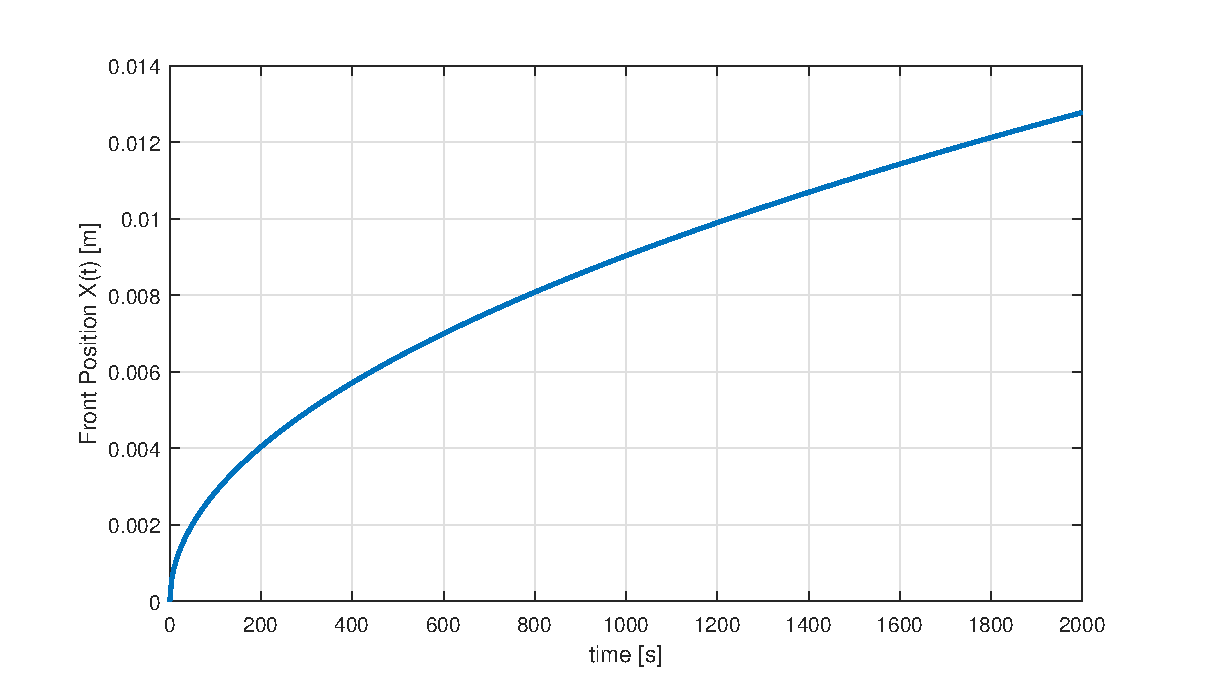
\includegraphics[width=0.9\linewidth]{figures/chapter_2/StefanFront.eps}
	\caption{Stefan melting front development over time}
	\label{fig:melt_front_movement}
\end{figure}


\section{Structural Mechanics}
\label{chap:solid_mechanics}
The main idea of structural mechanics is that a material deforms under a load. This gives rise to shear and normal stress in the material. It is usually enough to consider materials to behave linearly. This gives rise to the classical Hooke's law, which can be generalized for a multidimensional object. Continuum mechanics also needs to be considered for the derivation, but for simplicity, it is not discussed in this thesis.

\begin{figure}[ht]
	\centering
	\includegraphics[width=0.8\linewidth]{figures/chapter_2/StretchedBar.png}
	\caption{One-dimentional Hooke's law illustration}
	\label{fig:stretched_bar}
\end{figure}
First considering the one-dimensional case as illustrated in figure \ref{fig:stretched_bar}. A simple bar of length $L$ with cross-sectional area $S$ is subjected to a load $P$. Under this load, the bar stretches in the longitudinal direction by $\Delta L$ and contracts by $\Delta S$ in the perpendicular direction. Classical Hooke's law states that this stretching can be determined, as shown in equation \ref{eq:hookes_law} \cite{Lubliner_Papadopoulos_2014}. The contraction can also be computed from equation \ref{eq:hookes_law_contraction}, where $\nu$ is Poisson's ratio.
\begin{subequations}
	\begin{alignat}{2}
		\frac{\Delta L}{L} &= \frac{1}{E}\frac{P}{S} 
		\label{eq:hookes_law} \\
		\frac{\Delta S}{S} &= \nu\frac{\Delta L}{L}=\nu\frac{1}{E}\frac{P}{S} 
		\label{eq:hookes_law_contraction}
	\end{alignat}
\end{subequations}

Equation \ref{eq:hookes_law} is most commonly written as $\sigma=E\epsilon$ where $\sigma=P/S $ and $\epsilon=\Delta L/L$. In solid mechanics, the strain is usually $\mathcal{O}(10^{-3})$ while Young's modulus $E$ is usually $\mathcal{O}(10^6)$. Assuming the rod returns to its original form after the load is released, Hooke's law can be generalized and derived through continuum mechanics, and the linear, elastic material model can be determined. Equation \ref{eq:linear_elastic_material} shows this.
\begin{equation}
	\sigma=\lambda\text{tr}(D)\mathbf I + 2\mu D
	\label{eq:linear_elastic_material}
\end{equation}

The linear elastic model of materials introduces so-called Lam\'{e} parameters $\lambda$ and $\mu$ which can be calculated for each material, given its material properties are known, as shown in the equations \ref{eq:lame_equations}. It also introduces $D$, the small-strain tensor defined in equation \ref{eq:small_strain_tensor}.
\begin{subequations}
	\begin{equation}
		D =
		\begin{bmatrix}
			\epsilon_{xx} & \epsilon_{xy}  & \epsilon_{xz} \\
			\epsilon_{yx} & \epsilon_{yy}  & \epsilon_{xz} \\
			\epsilon_{zx} & \epsilon_{zy}  & \epsilon_{xz}
		\end{bmatrix}
		\label{eq:small_strain_tensor}
	\end{equation}
	\begin{equation}
		\lambda = \frac{\nu E}{(1+\nu)(1-2\nu)} \qquad \mu = \frac{E}{2(1+\nu)}
		\label{eq:lame_equations}
	\end{equation}
\end{subequations}

Considering a three-dimensional case, stress occurs in six ways. Three in the normal directions, and three in the shear planes. A compliance matrix can be found for the system $\epsilon=\mathbf{C}^{-1}\sigma$ can be determined for a general material as shown in equation \ref{eq:elasticity_matrix}, which includes the shear modulus $G_{ij}$ \cite{Lubliner_Papadopoulos_2014}.
\begin{equation}
	\mathbf{C}^{-1}=\begin{bmatrix}
		\frac{1}{E_x} & \frac{\nu_{xy}}{E_x} & -\frac{\nu_{xz}}{E_x} & 0 & 0 & 0 \\
		-\frac{\nu_{yx}}{E_y} & \frac{1}{E_y} & -\frac{\nu_{yz}}{E_y} & 0 & 0 & 0 \\
		-\frac{\nu_{zx}}{E_z} & -\frac{\nu_{zy}}{E_z} & -\frac{1}{E_z} & 0 & 0 & 0 \\
		0 & 0 & 0 & \frac{1}{G_{yz}} & 0 & 0 \\
		0 & 0 & 0 & 0 & \frac{1}{G_{xz}} & 0 \\
		0 & 0 & 0 & 0 & 0 & \frac{1}{G_{xy}} \\
	\end{bmatrix}
	\label{eq:elasticity_matrix}
\end{equation}

Often, the materials are isotropic which gives the material uniform material properties in each direction. As in some cases, such as in 2D, the $z$ component of stress and strain are equal to or negligible. This simplifies the matrix as shown in \ref{eq:plane_stress} for plane stress
\begin{equation}
	\mathbf C^{-1} = \frac{1}{E}\begin{pmatrix}
		1 & -\nu & 0 \\
		-\nu & 1 & 0 \\
		0 & 0 & 2(1+\nu)
	\end{pmatrix}
	\label{eq:plane_stress}
\end{equation}
or to the equation shown in \ref{eq:plane_strain} for plane strain \cite{Lubliner_Papadopoulos_2014}.
\begin{equation}
	\mathbf C = \frac{E}{1+\nu} \begin{pmatrix}
		\frac{1-\nu}{1-2\nu} & \frac{\nu}{1-2\nu} & 0 \\
		\frac{\nu}{1-2\nu} & \frac{1-\nu}{1-2\nu} & 0 \\
		0 & 0 & \frac{1}{2}
	\end{pmatrix}
	\label{eq:plane_strain}
\end{equation}


\section{Methods for Optimization}
\label{chap:methods_for_optimization}
In the context of engineering, the goal of optimization is to maximize or minimize one or more properties, possibly with a set of constraints. Typical examples include maximizing the stiffness of a frame while keeping the design below a weight requirement, or minimizing the mass of a bridge while ensuring the maximum stress is below some critical limit. In optimization, a maximum is equivalent to a minimum \cite{Kochenderfer_Wheeler_2019}. This allows the same optimization methods to be used for any function.
\begin{equation}
	\begin{matrix}
		\max_x f(x) \\
		\text{is equivalent to} \\
		\min_x -f(x)
	\end{matrix}
\end{equation}

In optimization, a constraint limits the design space of possible solutions \cite{Kochenderfer_Wheeler_2019}. Figure \ref{fig:constraint_example} shows a function with a global and local minimum. The $\chi$ variable denotes the constraint limiting the design space, and $x^*$ is the optimum that fulfills the design criteria.
\begin{figure}[ht]
	\centering
	\includegraphics[width=0.6\linewidth]{figures/chapter_2/ContraintExample.png}
	\caption{Example of a constraint limiting the design space \cite{Kochenderfer_Wheeler_2019}}
	\label{fig:constraint_example}
\end{figure}

\subsection*{Constrained Optimization}
This section will consider the following system.
\begin{equation}
	\begin{split}
		\min_x \quad &f(\mathbf x) \\
		\text{subject to} \quad & h(\mathbf x) = \mathbf 0\\
		& g(\mathbf x) \leq \mathbf 0
	\end{split}
\end{equation}
As was briefly introduced, constrained optimization has a function that has had its design space limited by one or more constraints. In such a situation, Lagrange multipliers can be used. The idea behind Lagrange multipliers is to find the point where the gradient of the function and constraint are aligned \cite{Kochenderfer_Wheeler_2019}. Equation \ref{eq:aligned_gradients} shows the condition for aligned gradients where $\lambda$ is the Lagrange multiplier. The purpose of the Lagrange multiplier is to scale the gradient, as while they may be aligned, they may not be the same size magnitude. Equation \ref{eq:lagrangian_eq} is the Lagrangian which is a function of both the design variables and the constraint. By finding $\nabla\mathcal{L}(\mathbf{x},\lambda) = \mathbf{0}$, the gradient condition is met, and a critical point is found \cite{Kochenderfer_Wheeler_2019}. 
\begin{subequations}
	\begin{equation}
		\nabla f(\mathbf{x})=\lambda\nabla h(\mathbf{x})
		\label{eq:aligned_gradients}
	\end{equation}
	\begin{equation}
		\mathcal{L}(\mathbf{x},\lambda) = f(\mathbf{x}) - \lambda h(\mathbf{x})
		\label{eq:lagrangian_eq}
	\end{equation}
\end{subequations}

The above formulation is for equality constraints. This means the critical point is assumed to be on the boundary of the constraint. However, if an inequality constraint is used instead, it may be that the critical point is simply where the gradient zero for the $f(\mathbf x)$. In this case, the constraint is considered "inactive" \cite{Kochenderfer_Wheeler_2019}. Equation \ref{eq:aligned_gradients_inequality} and \ref{eq:lagrangian_ineq} show a slight change in the Lagrangian, however, the idea is the same. $\mu$ is a non-negative Lagrange multiplier to ensure the constraint holds. 
\begin{subequations}
	\begin{equation}
		\nabla f(\mathbf{x})+\mu\nabla g(\mathbf{x}) = \mathbf 0
		\label{eq:aligned_gradients_inequality}
	\end{equation}
	\begin{equation}
		\mathcal{L}(\mathbf{x},\lambda) = f(\mathbf{x}) + \mu g(\mathbf{x})
		\label{eq:lagrangian_ineq}
	\end{equation}
\end{subequations}

To optimize the Lagrangian, a new solution strategy is required as shown in equation \ref{eq:solve_lagrangian_ineq}. This formulation is called the primal problem.
\begin{equation}
	\min_x \max_{\mu\geq 0}\mathcal{L}(\mathbf x, \mu)
	\label{eq:solve_lagrangian_ineq}
\end{equation}

To ensure a valid solution, the Kanush-Kuhn-Tucker (KKT) conditions \cite{Kuhn_Tucker_2013} must be satisfied. These are \ref{eq:point_feasible} which states the point is feasible, meaning the constraint is satisfied. Equation \ref{eq:penalty_in_right_direction} that states the penalty is in the right direction. Equation \ref{eq:boundary_feasibility} states that either the point is on the boundary $g(\mathbf x) = 0$, or $\mu = 0$. Lastly, equation \ref{eq:aligned_gradients_inequality_at_point} states that if the constraint is active, the contours of $f$ and $g$ are aligned, or $\mu = 0$ which recovers $\nabla f(\mathbf x^*) = 0$ \cite{Kochenderfer_Wheeler_2019}. 
\begin{subequations}
	\begin{alignat}{4}
		g(\mathbf x^*) &\leq 0
		\label{eq:point_feasible} \\
		\mu &\geq 0
		\label{eq:penalty_in_right_direction} \\
		\mu g(\mathbf x^*) &= 0
		\label{eq:boundary_feasibility} \\
		\nabla f(\mathbf x^*) + \mu \nabla g(\mathbf x^*) &= \mathbf 0
		\label{eq:aligned_gradients_inequality_at_point}
	\end{alignat}
\end{subequations}

\subsection*{Bisection Method}
The bisection method is a bracketing method that closes in on a root $y$. While it is a simple method, it is guaranteed to converge if the starting region brackets the root, and the function is continuous. First, a region $[a,b]$ has to be found which contains at least one root. This can be done by finding a point above the root, and another below. Assuming the function is continuous, then according to the intermediate value theorem, there must be a value between the bracketing points $[a,b]$ that satisfies $f(x) = y$ \cite{Kochenderfer_Wheeler_2019}. As is illustrated in figure \ref{fig:bisection_method}, the bisection method works by evaluating a middle point $c=(a+b)/2$ and selecting a new bracket that the root is still inside of. Note however that the function has five roots in the initial bracket, but it only converges to one.
\begin{figure}[ht]
	\centering
	\includegraphics[width=0.9\linewidth]{figures/chapter_2/Bisection.png}
	\caption{Illustration of the bisection method for finding the root of a function \cite{Kochenderfer_Wheeler_2019}}
	\label{fig:bisection_method}	
\end{figure}

\subsection*{Newton-Raphson Method}
The Newton-Raphson method, commonly known as the Newton method, is a second-order method that not only finds a decent direction but also predicts how far to step in that direction. Newton's method is an iterative scheme based on a second-order Taylor expansion shown in equation \ref{eq:2nd-order_taylor} and then taking its derivative \ref{eq:taylor_derivative} and then solving for $x$ which is used as a new guess $x^{(k+1)}$ as shown in equation \ref{eq:update_guess} \cite{Kochenderfer_Wheeler_2019}. Note that equation \ref{eq:update_guess} divides by the second derivative, giving rise to the condition that the second derivative is non-zero.
\begin{subequations}
	\begin{equation}
		q(x) = f(x^{(k)}) + (x - x^{(k)})f'(x^{(k)})+\frac{(x-x^{(k)})^2}{2}f''(x^{(k)})
		\label{eq:2nd-order_taylor}
	\end{equation}
	\begin{equation}
		\frac{\partial q}{\partial x} = f'(x^{(k)}) + (x-x^{(k)})f''(x^{(k)}) = 0
		\label{eq:taylor_derivative}
	\end{equation}
	\begin{equation}
		x^{(k+1)} = x^{(k)} - \frac{f'(x^{(k)})}{f''(x^{(k)})}
		\label{eq:update_guess}
	\end{equation}
\end{subequations} 

While Newton's method has quadratic convergence, it does have some cases where it will fail to converge, as illustrated in figure \ref{fig:newton_failure}. The first is oscillations, where the new guesses continually overshoot the local minimum. The second is overshoot which occurs when the new guess goes beyond the local minimum. The last occurs when the second derivative is negative, causing the new guess to diverge. Therefore, in Newton's method, a good initial guess is often necessary \cite{Kochenderfer_Wheeler_2019}.
\begin{figure}[ht]
	\centering
	\includegraphics[width=0.9\linewidth]{figures/chapter_2/NewtonFailure.png}
	\caption{Some common failure cases for Newton's method \cite{Kochenderfer_Wheeler_2019}}
	\label{fig:newton_failure}
\end{figure}

\subsection*{Line Search}
The line search method doesn't compute a descent direction, but rather it computes a step size $\alpha$ which decides how far to step in the decent direction, as shown in equation \ref{eq:linesearch_min}. The search direction $\mathbf d$ can be computed from Newton's method for example.
\begin{equation}
	\min_\alpha f(\mathbf x + \alpha \mathbf d)
	\label{eq:linesearch_min}
\end{equation}

The step size can be computed exactly, but its computation is very expensive. Instead, an approximate $\alpha$ can be found quickly using a line search algorithm such as the backtracking algorithm \cite{Kochenderfer_Wheeler_2019}, and then a new search direction can be computed. 

One common line search algorithm is the back-tracking algorithm. This uses a condition called the Armijo condition, shown in equation \ref{eq:armijo_condition}, which ensures a sufficient decrease in the objective function \cite{Kochenderfer_Wheeler_2019}. Note that $\beta\in[0,1]$.
\begin{equation}
	f(\mathbf x^{(k+1)}) \leq f(\mathbf x^(k)) + \beta\alpha\nabla_{\mathbf d^{(k)}}f(\mathbf x^{(k)})
	\label{eq:armijo_condition}
\end{equation}

\subsection*{Multi-functional Optimization}
Multi-functional optimization, also known as multi-objective optimization, is the optimization of two or more functions that may have conflicting optimal points. This requires the designer to find a trade-off between the objective functions. This gives rise to the idea of Pareto optimality.

A design is said to be Pareto optimal when it is no longer possible to improve one objective without worsening another \cite{Kochenderfer_Wheeler_2019}. With a set of Pareto optimal points, a Pareto frontier is constructed. Figure \ref{fig:pareto_front} shows a Pareto front that also has weakly Pareto-optimal points. Any point taken from the front is a valid Pareto-optimal design, but each will have a trade-off between each function.
\begin{figure}[ht]
	\centering
	\includegraphics[width=0.65\linewidth]{figures/chapter_2/ParetoFront.png}
	\caption{A Pareto front (blue) with weakly Pareto-optimal points (red) \cite{Kochenderfer_Wheeler_2019}}
	\label{fig:pareto_front}
\end{figure}

Many methods exist to obtain Pareto-optimal points, but only two methods will be discussed here. The first is the constraint method. In this method, all but one objective function is constrained \cite{Kochenderfer_Wheeler_2019}. This essentially converts the multiple functions into a single constraint function which can be optimized using constraint optimization techniques.
\begin{equation}
	\begin{split}
		\min_x \quad f_1(x) \\
		\text{subject to} \quad f_2(x) & \leq c_2 \\
		& \vdots \\
		f_n(x) &\leq c_n
	\end{split}
\end{equation}

The drawback to the constrained method, and the motivation for using the next method, is that the constraints may not be known ahead of time. This could be resolved by minimizing both functions independently and finding the maximum of each function with respect to the other functions' minimums. However, this can be cumbersome. Instead, the weight method can be used. The weight method works but weighing each objective function by an importance factor as shown in equation \ref{eq:weight_method}. This method also converts the multiple objectives into a single function but doesn't require constraint optimization techniques, or having to determine the constraints. However, one drawback to this method is that this method cannot find Pareto optimal points that are in a convex region, as illustrated in figure \ref{fig:weight_method_failure}.
\begin{figure}[t]
	\centering
	\includegraphics[width=0.65\linewidth]{figures/chapter_2/WeightMethodFailure.png}
	\caption{Weight method failure on convex regions}
	\label{fig:weight_method_failure}
\end{figure}
\begin{equation}
	f(x) = \mathbf w^T \mathbf f(x)
	\label{eq:weight_method}
\end{equation}


\section{Finite Element Method}
\label{chap:finite_element_method}
The finite element method (FEM) is a numerical method for solving boundary value problems (BVP). As a minor prelude, the Sobolev space $\mathcal{H}^k(\Omega)$ needs to be defined. The Sobolev space is defined as the set of functions that are square integrable in the domain $\Omega$ (meaning they are in the $\mathcal{L}_2(\Omega)$ space) and has $k$ square integrable derivatives. The Sobolev space is therefore defined in \ref{eq:sobolev_space}, where $\alpha=\alpha_1,\dots,\alpha_d$ and $|\alpha|=\alpha_1+\dots+\alpha_d$. Also defined is $\mathcal{H}_0^k(\Omega)$ which simply has values that vanish on the boundaries \cite{Donea_Huerta_2004}.
\begin{subequations}
	\begin{equation}
		\mathcal{H}^k(\Omega) = \left \{ u\in \mathcal{L}(\Omega) \quad \middle | \quad \partial_x^\alpha u \in \mathcal{L}^2(\Omega) \quad \forall |\alpha|\leq k \right \} 
		\label{eq:sobolev_space}
	\end{equation}
	\begin{equation}
		\mathcal{H}_0^k(\Omega) = \left \{ u\in \mathcal{H}^k(\Omega) \quad | \quad u=0 \text{ on } \Gamma \right \}
	\end{equation}
\end{subequations}

To define the variational form of a BVP, the notion of trial and weighting function spaces is needed. The weighting functions, denoted as $\mathcal{V}$ and shown in equation \ref{eq:weighting_function_space}, is the set of functions in $\mathcal{H}^1(\Omega)$ with values that vanish on the Dirichlet boundaries $\Gamma_D$ \cite{Donea_Huerta_2004}.
\begin{equation}
	\mathcal{V}=\left \{ w\in\mathcal{H}^1(\Omega) \ \middle | \ w = 0 \ \text{on} \ \Gamma_D \right \}
	\label{eq:weighting_function_space}
\end{equation}

The trial function space, defined in equation \ref{eq:trial_function_space}, is the set of functions in $\mathcal{H}^1$ that satisfy the Dirichlet value $u_D$ on the Dirichlet boundaries \cite{Donea_Huerta_2004}. 
\begin{equation}
	\mathcal{S}=\left \{ u\in\mathcal{H}^1(\Omega) \ \middle | \ u = u_D \ \text{on} \ \Gamma_D \right \}
	\label{eq:trial_function_space}
\end{equation}

These function spaces contain an infinite number of functions, so in FEM, a finite-dimensional subset $\mathcal{V}^h$ and $\mathcal{S}^h$, that can approximate $\mathcal{V}$ and $\mathcal{S}$, is chosen \cite{Donea_Huerta_2004}. Not only that but the domain is also discretized into element domains. Equation \ref{eq:function_spaces_finite} shows convenient function spaces which make use of polynomial interpolation functions $\mathcal{P}_m(\Omega)$ of order $m$ which are defined for different types of element $e$ \cite{Donea_Huerta_2004}.
\begin{subequations}
	\begin{equation}
		\mathcal{V}^h=\left \{ w\in\mathcal{H}^1(\Omega) \ \middle | \ w|_{\Omega^e}\in\mathcal{P}_m(\Omega)^e \ \forall e \ \text{and} \ w = 0 \ \text{on} \ \Gamma_D \right \}
	\end{equation}
	\begin{equation}
		\mathcal{S}^h=\left \{ u\in\mathcal{H}^1(\Omega) \ \middle | \ u|_{\Omega^e}\in\mathcal{P}_m(\Omega)^e \ \forall e \ \text{and} \ u = u_D \ \text{on} \ \Gamma_D \right \}
	\end{equation}
	\label{eq:function_spaces_finite}
\end{subequations}

Dirichlet boundary conditions, which have already been mentioned, impose a value on the boundary $u = u_D \ \text{on} \ \Gamma_D$. Neumann conditions impose a gradient or flux on the boundary $\frac{\partial u}{\partial n} = \mathbf n  \cdot \nabla u = h \ \text{on} \ \Gamma_N$.

With that, the weak form can now be derived. The weak form is found by multiplying the equation with a weighting function $w$ and integrating it over the domain $\Omega$. For the Poisson equation, equation \ref{eq:poisson_weak_form} shows the derivation. The second step shows the application of integration by parts and the result after using Gauss' theorem. Note that a Neumann boundary condition naturally arises from this formulation.
\begin{equation}
	\begin{split}
		-\int_\Omega w\nabla^2 u \ d\Omega &= \int_\Omega w f \ d\Omega \\
		-\int_\Omega (\nabla\cdot(w\nabla u)-\nabla w \cdot \nabla u) \ d\Omega &= \int_\Omega w f \ d\Omega \\
		\int_\Omega \nabla w \cdot \nabla u \ d\Omega &= \int_\Omega w f \ d\Omega + \int_{\Gamma_N} wh \ d\Gamma
	\end{split}
	\label{eq:poisson_weak_form}
\end{equation}

Some shorthand notations can be used for simplification.
\begin{equation}
	\begin{split}
		a(w,u) &= \int_\Omega \nabla w \cdot \nabla u \ d\Omega \\
		(w,f) &= \int_\Omega w f \ d\Omega \\
		(w,h)_{\Gamma_N} & = \int_{\Gamma_N} wh \ d\Gamma
	\end{split}
	\label{eq:bilinear_forms}
\end{equation}

The Galerkin method can now be applied which discretizes the space into a finite subset of the full function spaces and reads as follows, where $u^h(\mathbf x)=\sum_{e=1}^{N_e}N_e(\mathbf x)u_e$. 

Find $u^h\in\mathcal{S}^h$ such that $a(w^h,u^h) = (w^h,f) + (w^h,h)_{\Gamma_N}$    $\forall w^h\in\mathcal{V}^h$

\begin{figure}[t]
	\centering
	\includegraphics[width=0.75\linewidth]{figures/chapter_2/QuadElement.png}
	\caption{1st order quadrilateral element mapping}
	\label{fig:quad_element}
\end{figure}
The shape functions $N_e$ are defined for each element. For each element, there are $n$ nodes and an equal number of shape functions. The shape functions are constructed in a way that they are equal to one on their node, and zero on each other node. For example, figure \ref{fig:quad_element} shows a 1st-order quadrilateral element, which has the shape functions shown in equation \ref{eq:quad_shape_functions}.
\begin{equation}
	\begin{split}
		N_1 = \frac{1}{4}(1-\xi)(1-\eta) \\
		N_1 = \frac{1}{4}(1+\xi)(1-\eta) \\
		N_1 = \frac{1}{4}(1+\xi)(1+\eta) \\
		N_1 = \frac{1}{4}(1-\xi)(1+\eta)
	\end{split}
	\label{eq:quad_shape_functions}
\end{equation}

By defining the elements in a separate domain, these need to be mapped to the global domain. This leads to an isoparametric mapping for the quadrilateral element \cite{Donea_Huerta_2004}, as shown in equation \ref{eq:isoparametric_mapping}.
\begin{equation}
	\begin{Bmatrix} x \\ y \end{Bmatrix} = \sum_{i=1}^4 N_i(\xi,\eta)\begin{Bmatrix} x_i \\ y_i \end{Bmatrix}, \quad \text{and} \quad u^h(x,y)=\sum_{i=1}^4 N_i(\xi,\eta)u_i
	\label{eq:isoparametric_mapping}
\end{equation}

By defining the reference elements, it is also possible to efficiently compute their integrals using Gaussian quadrature. Equation \ref{eq:gaussian_quadrature} shows the rule where $w_i$ are weights for each Gauss point $[\xi_i,\eta_i]$ \cite{McClarren_2018}, given $n_p$ Gauss points.
\begin{equation}
	\int_{-1}^{1}f(x)dx \approx \sum_{i=1}^{n_p}w_i f(\xi_i,\eta_i)
	\label{eq:gaussian_quadrature}
\end{equation}

All of the above is related to spatial discretization. For transient problems, however, time discretization is needed. The theta-family methods, shown in equation \ref{eq:theta_family}, are some of the most common first-order time discretization techniques \cite{Donea_Huerta_2004}. Some common methods coming from this are the backward ($\theta=1$) and forward ($\theta=0$) Euler methods, as well as the Crank-Nicolson ($\theta = 1/2$) method.
\begin{equation}
	\frac{\partial u}{\partial t} \approx \frac{u(t^{n+1})-u(t^n)}{\Delta t} = \theta u_t(t^{n+1}) + (1 - \theta)u_t(t^n)
	\label{eq:theta_family}
\end{equation}

Equation \ref{eq:theta_family} can also be expressed in the incremental form, shown in equation \ref{eq:incremental_form}, in which the incremental unknown $\Delta u = u^{n+1}-u^n$ is solved for. This form is often preferred \cite{Donea_Huerta_2004}. Note that $u_t=\frac{\partial u}{\partial t}$
\begin{equation}
	\frac{\Delta u}{\Delta t}-\theta\Delta u_t = u_t^n 
	\label{eq:incremental_form}
\end{equation}

The full discretization of the time-dependent poisson equation is given in equation \ref{eq:time_dependent_poisson_weak_form}. The discretization makes use of the backward Euler method ($\theta = 1$). Note that after spatial discretization, the derivation makes use of the bilinear forms defined in equation \ref{eq:bilinear_forms}.
\begin{equation}
	\begin{split}
		\frac{u^{n+1}-u^n}{\Delta t} &= f^{n+1}+\nabla^2 u^{n+1} \\
		u^{n+1}-\Delta t \nabla^2 u^{n+1} &= \Delta t f^{n+1}+u^n \\
		(w,u^{n+1}) -\Delta t \ a(w,u^{n+1}) &=\Delta t(w,f) +\Delta t(w,h)_{\Gamma_N}+ (w,u^n)
	\end{split}
	\label{eq:time_dependent_poisson_weak_form}
\end{equation}


\section{Automatic Differentiation}
\label{chap:auto_diff}
Automatic differentiation (AD) is a powerful numerical tool that is capable of computing exact derivatives (to machine precision) of computer programs. This is possible based on the idea that computer programs are made up of elementary operations such as multiplication, division, addition and subtraction \cite{Kochenderfer_Wheeler_2019}. The key to AD is the application of the chain rule \cite{Kochenderfer_Wheeler_2019}, shown in equation \ref{eq:chain_rule}.
\begin{equation}
	\frac{d}{dx}f(g(x)) = \frac{df}{dg}\frac{dg}{dx}
	\label{eq:chain_rule}
\end{equation}

Automatic differentiation can be implemented through operator overloading and the use of dual numbers \cite{Kochenderfer_Wheeler_2019}. Dual numbers are similar to complex numbers, in that they are expressed as $a + b\epsilon $. The variable $\epsilon^2$ is defined to be 0 and the values $a$ and $b$ are both real numbers. The operations performed on dual numbers act as normal, as shown below in equation \ref{eq:dual_number_basic_ops} \cite{Kochenderfer_Wheeler_2019}.
\begin{subequations}
	\begin{equation}
		(a + b\epsilon) + (c + d\epsilon) = (a + c) + (b + d)\epsilon
		\label{eq:dual_number_addition}
	\end{equation}
	\begin{equation}
		(a + b\epsilon) \times (c + d\epsilon) = (ac) + (ad + bc)\epsilon
		\label{eq:dual_number_multiplication}
	\end{equation}
	\label{eq:dual_number_basic_ops}
\end{subequations}

Dual numbers are powerful tools when passed into any smooth function $f$. By Taylor expansion, it can be shown that the function evaluation, as well as its derivative, can be found \cite{Kochenderfer_Wheeler_2019}. 
\begin{equation}
	\begin{split}
		f(x) &= \sum_{k=0}^\infty \frac{f^{(k)}(a)}{k!}(x-a)^k \\
		f(a+b\epsilon) &= \sum_{k=0}^\infty \frac{f^{(k)}(a)}{k!}(a+b\epsilon-a)^k \\
		&= \sum_{k=0}^\infty \frac{f^{(k)}(a)b^k\epsilon^k}{k!} \\
		&= f(a) + bf'(a)\epsilon + \epsilon^2\sum_{k=2}^\infty \frac{f^{(k)}(a)b^k}{k!}\epsilon^{(k-2)} \\
		&= f(a) + bf'(a)\epsilon
	\end{split}
	\label{eq:dual_taylor_expansion}
\end{equation}

Furthermore, AD can be used in either forward or reverse mode. Consider a generic problem where the Jacobian $\frac{df_i}{dx_j}$ is to be computed, where $i\in[1,2,\dots,n]$ and $j\in[1,2,\dots,m]$. Forward mode AD is capable of computing the Jacobian column-by-column $\frac{d\mathbf{f}}{dx_j}$. In reverse mode, the Jacobian is computed row-by-row $\ \frac{df_i}{d\mathbf{x}}$. How this is achieved will be discussed in the following sections. For the following examples, the derivative of the function in equation \ref{eq:auto_diff_example} will be evaluated. 
\begin{equation}
	f(x_1,x_2) = x_1x_2 + x_1\sin(x_2)
	\label{eq:auto_diff_example}
\end{equation}

\subsection*{Forward Mode}
As was mentioned, forward mode AD computes a Jacobian column-by-column. This means it is more efficient to use forward mode when $n < m$. The evaluation of equation \ref{eq:auto_diff_example} can be thought of visually as a directed acyclic graph (DAG), where each sub-evaluation is a vertex. The lines connecting each vertex can be thought of as where the derivatives are evaluated. The DAG for equation \ref{eq:auto_diff_example} is shown in figure \ref{fig:auto_diff_example_dag}.

With forward mode AD, a function can be differentiated with respect to a single variable in each forward pass. A forward pass is simply computing the DAG from left to right. To achieve this using dual numbers, the dual number for only one variable is '\emph{seeded}.' In this example $f(a,b)$, equation \ref{eq:auto_diff_forward}. In this example, $v_4$ and $v_5$ using equation \ref{eq:dual_number_multiplication} and $v_6$ used equation \ref{eq:dual_number_addition}. To compute the full derivative, two forward passes are required.
\begin{equation}
	\begin{split}
		v_1 &= a+1\epsilon \\
		v_2 &= b+0\epsilon \\
		v_3 &= \sin(b)+0\epsilon
	\end{split} \qquad
	\begin{split}
		v_4 &= v_1v_2=ab+b\epsilon \\
		v_5 &= v_1v_3 = a\sin(b) + \sin(b)\epsilon \\
		v_6 &= v_4 + v_5 = ab+a\sin(b) + (b + \sin(b))\epsilon 
	\end{split}
	\label{eq:auto_diff_forward}
\end{equation}

\subsection*{Reverse Mode}
Reverse mode AD computes a Jacobian row-by-row. This makes it more efficient when $m < n$. Reverse mode AD consists of a forward pass where the vertices and lines are computed, and a reverse accumulation pass. In this case, the lines are the derivatives of $v_j$ w.r.t $v_i$ rather than w.r.t the variable. 

The reverse pass requires the evaluation of equation \ref{eq:reverse_pass}. The parents ($p$) of vertex $i$ are all the forward vertices connected to $v_i$. For this example, $v_2$ has $v_3$ and $v_4$ as parents. From equation \ref{eq:reverse_pass}, it is clear that the entire DAG needs to be stored in memory to be able to compute the derivative. However, it is now also possible to compute the derivative w.r.t all the inputs. 
\begin{equation}
	\frac{\partial y}{\partial v_i}=\sum_{p\in \text{parent}(i)}\frac{\partial y}{\partial v_p}\frac{\partial v_p}{\partial v_i}
	\label{eq:reverse_pass}
\end{equation}


\begin{figure}[b]
	\centering
	\includegraphics[width=0.75\linewidth]{figures/chapter_2/AutomaticDifferentiation.png}
	\caption{Graph of equation \ref{eq:auto_diff_example}}
	\label{fig:auto_diff_example_dag}
\end{figure}                        \cleardoublepage    % 10-15 pages
    \chapter{State of the Art}
\label{chap:state_of_the_art}

\section{Cellular Structures}
\label{chap:cellular_structures}
Cellular structures are a relatively new kind of structure with promising properties that can be utilized in engineering, as they combine high stiffness with low mass. They are common in nature, such as in honeycombs, bone and wood. While they have been manufactured in the past using conventional approaches, such as using complex molds for casting \cite{Tao_Leu_2016}, their use in recent times has been accelerated due to the rise of additive manufacturing \cite{Jandyal_Chaturvedi_Wazir_Raina_Ul_Haq_2022}. Cellular structures can be broken into two categories. These are stochastic structures (foams) that have random non-repeating structures, and lattice structures which have repeating unit cells \cite{Tao_Leu_2016}. Lattice structures have been found to have superior properties when compared to foams, making them a promising solution to applications such as in lightweight structure design \cite{Tao_Leu_2016}. 

There is a multitude of different types of cells that can be used. Some common unit cells are shown in figure \ref{fig:unit_cells}. These cells are open cells with a height $h$, that are built up by struts with radius $r$.
\begin{figure}[ht]
    \centering
    \includegraphics[width=0.7\linewidth]{figures/chapter_3/UnitCells.png}
    \caption{A selection of unit cells \cite{Piacquadio_Soika_Schirp_Schröder_Filippeschi_2023}}
    \label{fig:unit_cells}
\end{figure}

To simulate cellular structures, without having to mesh each cell, they can be treated as materials. For this, researchers have worked on homogenizing each type of cell to give effective material properties \cite{Piacquadio_Soika_Schirp_Schröder_Filippeschi_2023}\cite{Bühring_Soika_Schirp-Schoenen_Schröder_2022}. In structural mechanics, this involves determining the elastic modulus in each direction, whereas, in thermal problems, it involves determining the conductivity in each direction with an embedded PCM. The cells are considered porous media with porosity $\epsilon$. The porosity can be defined as the proportion of void volume to the total volume, or one minus the solid volume fraction $\mathcal{X}$ \cite{Piacquadio_Soika_Schirp_Schröder_Filippeschi_2023}, as shown in equation \ref{eq:porosity_definition}.
\begin{equation}
    \epsilon = 1 - \mathcal{X} = 1 - \frac{V_\text{solid}}{V_\text{total}}
    \label{eq:porosity_definition}
\end{equation} 

\subsection*{Structural Properties}
For the structural properties, only the matrix (the cell itself) is considered. This is because the selected phase change material, \emph{paraffin}, has a very low elastic modulus, relative to the material of the cell. Not only that but when the phase change material is in its liquid phase, then it provides no stiffness to the cells. For this thesis, the $bcc$ and $f_2 cc,z$ cells have been considered, but any other homogenized unit cell could be used instead. The properties were obtained from \cite{Bühring_Soika_Schirp-Schoenen_Schröder_2022}.

For the selected cells, only the Young's moduli in each direction are required. Young's modulus is non-linear for the unit cells. Figure \ref{fig:youngs_modulus_bcc_e1} shows the non-linear nature of Young's modulus. This will later have an impact on the topology optimization because the intermediate densities will have a different impact on how the structure grows.
\begin{figure}[ht]
    \centering
    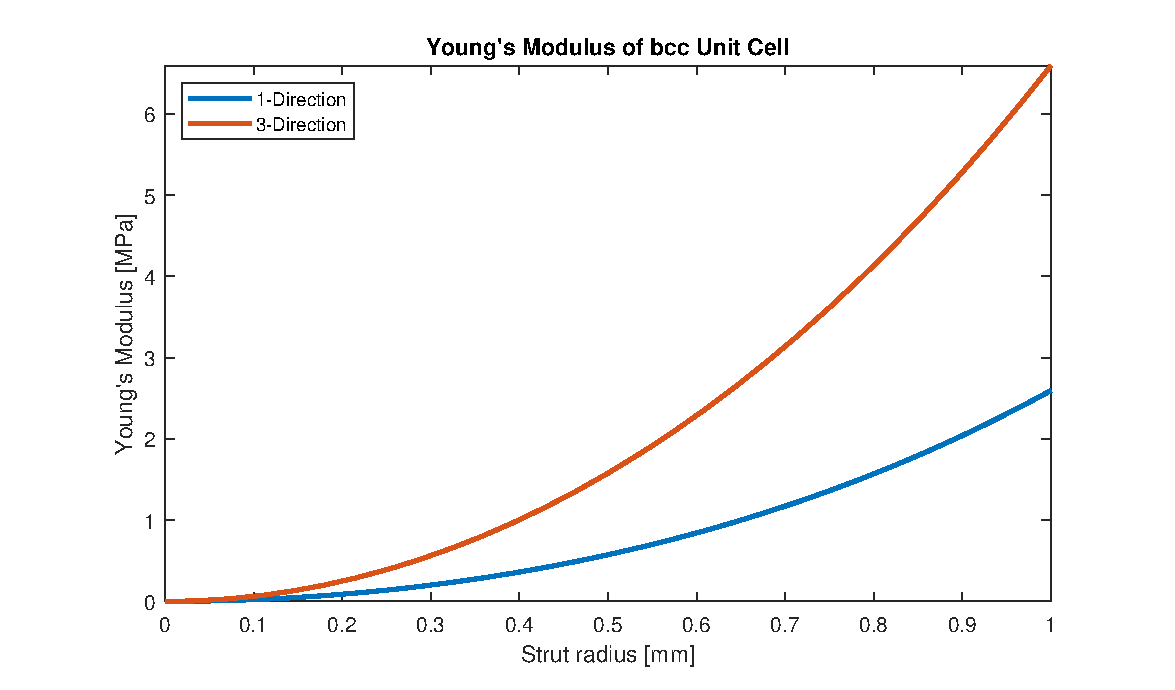
\includegraphics[width=0.9\linewidth]{figures/chapter_3/BCC_E1.eps}
    \caption{Young's Modulus of the BCC unit cell in each direction}
    \label{fig:youngs_modulus_bcc_e1}
\end{figure}


\subsection*{Thermal Properties}
The thermal properties of the unit cells are made up of both a highly conductive matrix (the cells themself), and a low-conductivity filler (phase change material). The cell properties are obtained from the master's thesis \cite{Piacquadio_Soika_Schirp_Schröder_Filippeschi_2023}. Again, this thesis only focuses on the $bcc$ and $f_2 cc,z$ cells, but any other homogenized unit cell could be used. The filler material is considered in these equations as it provides a non-negligible contribution to the thermal properties.

The required thermal properties that are needed are the effective thermal conductivity $k_{eff}$, the effective specific heat $c_{p, eff}$, and the effective latent heat $L_{eff}$. The specific heat and latent heat properties can be computed using the equations shown in equation \ref{eq:mixture_rules} which include the effective density $\rho_{eff}$ \cite{Piacquadio_Schirp-Schoenen_Mameli_Filippeschi_Schröder_2022}. Note that these equations all consider the porosity $\epsilon$.
\begin{subequations}
    \begin{equation}
        \rho_{eff} = \epsilon\rho_{\text{PCM}} + (1 - \epsilon)\rho_{\text{solid}}
    \end{equation}
    \begin{equation}
        c_{p, eff} = \epsilon\frac{\rho_\text{PCM}}{\rho_{eff}}c_{p,\text{PCM}} + (1 - \epsilon)\frac{\rho_\text{solid}}{\rho_{eff}}c_{p, \text{solid}} 
    \end{equation}
    \begin{equation}
        L_{eff} = \epsilon\frac{\rho_\text{PCM}}{\rho_{eff}}L_\text{PCM}
    \end{equation}
    \label{eq:mixture_rules}
\end{subequations}

Figure \ref{fig:thermal_properties} shows the properties of the $bcc$ unit cell as an example. Each of the properties is non-linear. Note that the effective latent heat is in terms of volume fraction, as this is important during the topology optimization. The specific heat curve is essentially a scaled version of the latent heat curve, so is not shown in the plots.
\begin{figure}[ht]
    \centering
    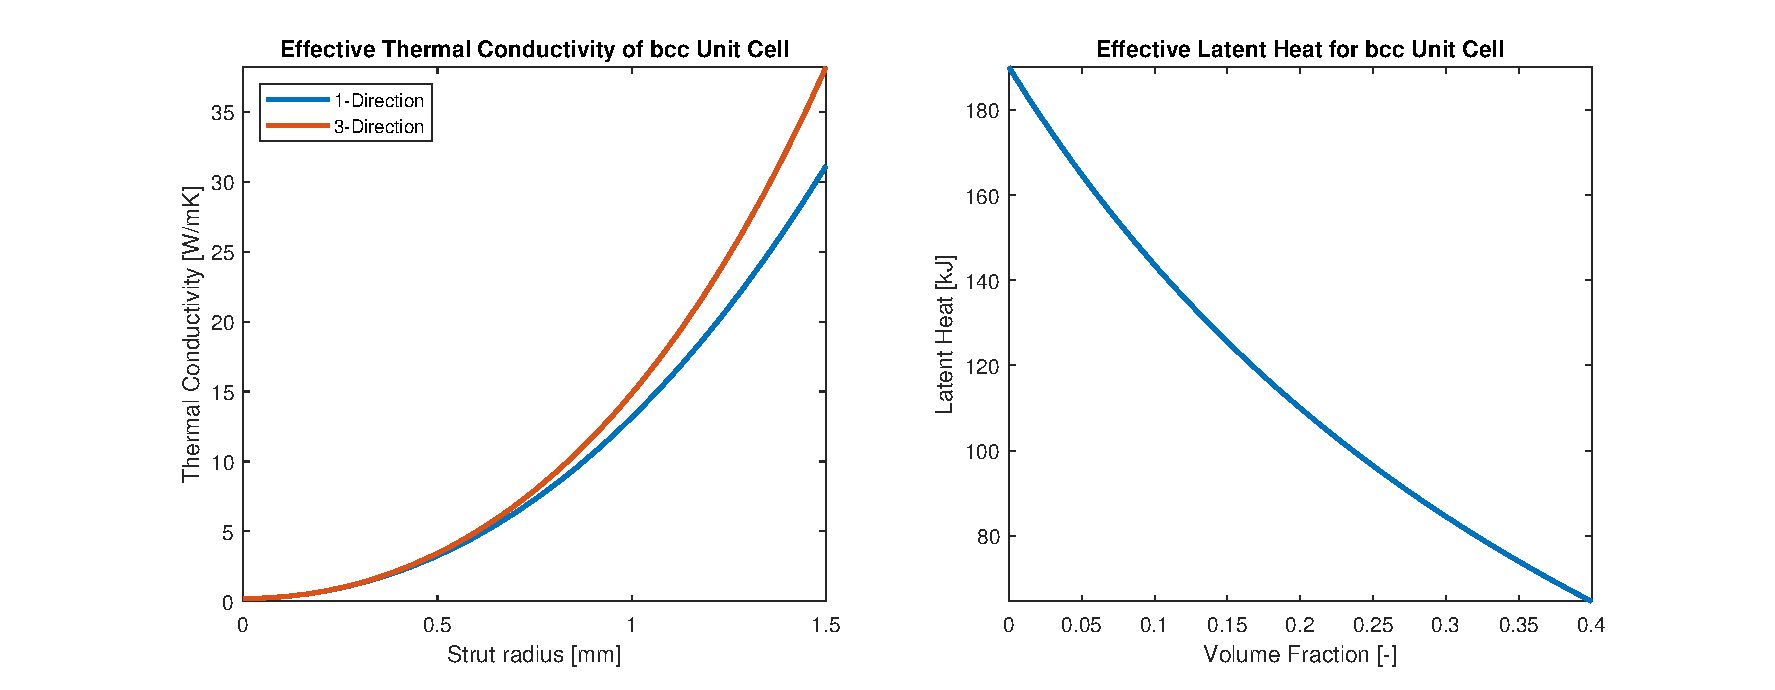
\includegraphics[width=0.95\linewidth]{figures/chapter_3/ThermalProperties.eps}
    \caption{Thermal properties of the $bcc$ unit cell}
    \label{fig:thermal_properties}
\end{figure}


\section{Latent Heat Energy Storage}
\label{chap:latent_heat_energy_storage}
Thermal energy storage is a method of storing heat in materials, either actively or passively, that can then be dissipated at a later time \cite{Cabeza_Martorell_Miró_Fernández_Barreneche_Cabeza_Fernández_Barreneche_2021}. One of the main uses currently is to assist the temporal and location mismatches between energy generation, and energy use. Thermal energy storage can also be used as a thermal management solution, where large amounts of heat may be generated irregularly, and can be dissipated passively over time.

A common thermal energy storage method is sensible heat energy storage. This method stores energy in a material without any phase change. The amount of sensible energy stored, $Q$, is expressed in equation \ref{eq:sensible_energy_storage} \cite{Cabeza_Martorell_Miró_Fernández_Barreneche_Cabeza_Fernández_Barreneche_2021}. Because this method involves no phase change, the best materials to select are those with a high specific heat $c_p$ and low cost. Materials such as water, oil and molten salts have been commonly used due to their availability and low cost. Note that the variable $m$ denotes the mass. Note that here $\Delta T = T - T_\text{ref}$, where $T_\text{ref}$ is the initial or ambient temperature.
\begin{equation}
    Q = m c_p \Delta T 
    \label{eq:sensible_energy_storage}
\end{equation}

In contrast to sensible heat energy storage, latent heat energy storage relies on the phase transition enthalpy $\Delta h$, or latent heat $L = \Delta h$, of a material to store vast amounts of energy for virtually no change in temperature \cite{Cabeza_Martorell_Miró_Fernández_Barreneche_Cabeza_Fernández_Barreneche_2021}. The total absorbed energy of the material can be expressed as shown in equation \ref{eq:total_sensible_energy}, which is the sum of sensible energy storage resulting in the solid and liquid phase, and the latent heat of melting. Latent heat energy storage materials are referred to as phase change materials. Note that the subscripts denote the solid phase $s$ or liquid phase $l$. Also note that $\Delta T_s = T_\text{melt} - T_\text{ref}$ and $\Delta T_f = T - T_\text{melt}$.
\begin{equation}
    Q = m c_{p,s}\Delta T_s + mL + m c_{p,l}\Delta T_l
    \label{eq:total_sensible_energy}
\end{equation}

Comparing the two methods, as shown in figure \ref{fig:sensible_vs_latent_storage}, the choice of energy storage method should depend on the application. When the temperature range is large, sensible energy storage can store much more energy, while in a narrow temperature range, latent heat energy storage is far superior. 
\begin{figure}[ht]
    \centering
    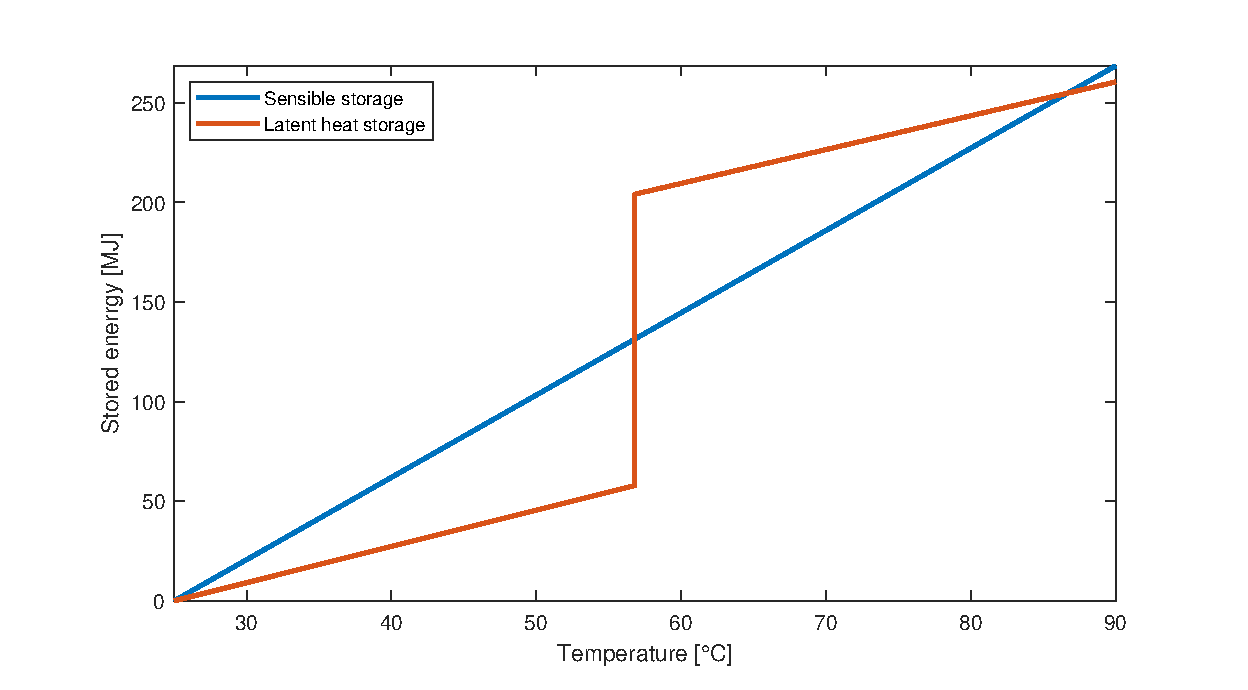
\includegraphics[width=0.7\linewidth]{figures/chapter_3/SensibleAndLatentStorage.eps}
    \caption{Sensible energy storage in water vs. the latent heat energy storage in paraffin}
    \label{fig:sensible_vs_latent_storage}
\end{figure}

\subsection*{Phase Change Materials}
The selection of phase change materials can be quite complex. The most important criteria are shown in table \ref{table:pcm_selection} \cite{Gadhave_Prabhune_Pathan_2020}. The most obvious selection criterion is the melting temperature of the material. This needs to be within the operating temperature, otherwise, it will simply act as a sensible heat storage medium. The next major selection criterion is the latent heat of the material. The higher, the more energy can be stored, and the longer the material remains around the melting temperature. Another very important property is the thermal conductivity. Having a low thermal conductivity would mean the temperature gradient in the domain could be quite high. This is not desirable when used in a cooling situation. 

The physical properties are also quite important to consider. If the phase change material is in a fixed volume, then the density change of the material could lead to very high pressures being sustained. It is for this reason that phase change materials are usually selected for solid-to-liquid phase change.
\begin{table}[ht]
    \centering
    \caption{Phase change material selection \cite{Gadhave_Prabhune_Pathan_2020}}
    \begin{tabular}{ c | c } 
        \hline
        \multirow{4}{*}{Thermal} & Melting temperature \\ & Latent heat \\ & Thermal conductivity \\ & Specific heat \\
        \hline
        \multirow{3}{*}{Physical} & High density \\ & Volume change \\ & Low vapour pressure \\
        \hline
        \multirow{3}{*}{Chemical} & Chemical stability \\ & Non-corrosiveness \\ & Non-flammability \\
        \hline
        \multirow{3}{*}{Economical} & Availability \\ & Cost \\ & Commercial viability \\
        \hline
    \end{tabular}
    \label{table:pcm_selection}
\end{table}

Some common phase change materials are shown in figure \ref{fig:pcm_selection}. A particularly good phase change material is water/ice, due to it having a high melting enthalpy and high availability. However, at ambient temperatures, the ice would have already melted, and therefore, only act as a sensible heat energy storage medium. Instead, paraffins have become a promising phase change material. Paraffins are organic materials that are a mixture of straight-chain n-alkanes \cite{Reza_Vakhshouri_2020}. By increasing the chain length, the melting temperature, as well as the latent heat increases \cite{Reza_Vakhshouri_2020}. This allows the material to be fine-tuned, to a degree, to the specific low-temperature use case. Of course, the other selection criteria also need to be considered.
\begin{figure}[ht]
    \centering
    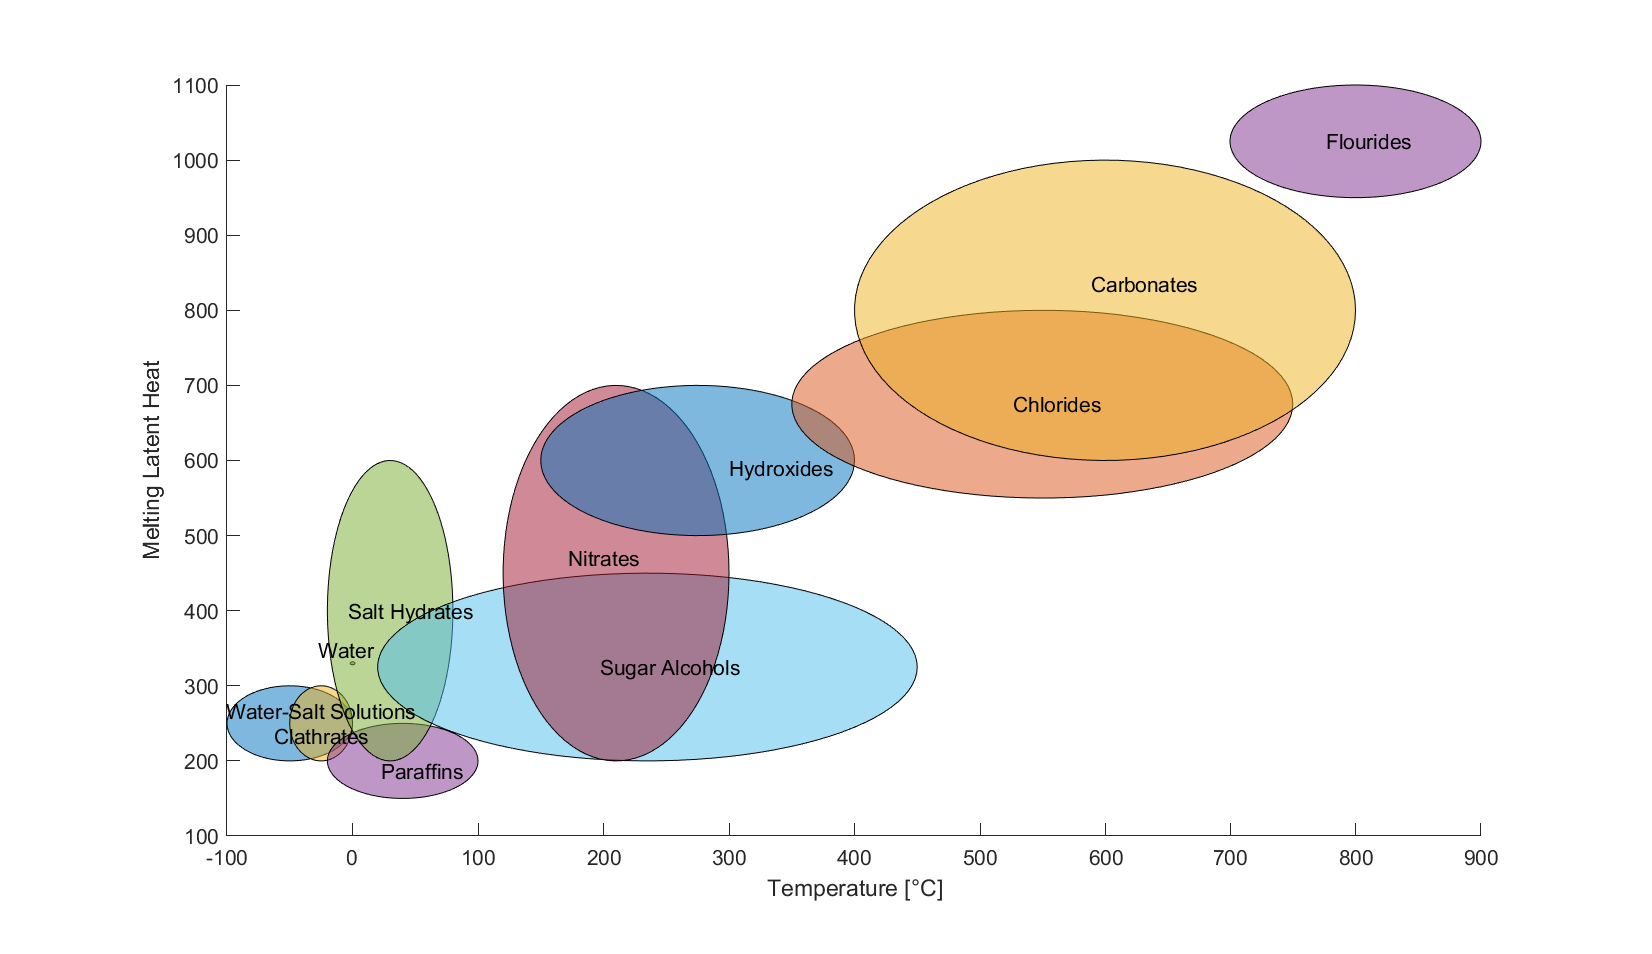
\includegraphics[width=0.8\linewidth]{figures/chapter_3/PCMs.eps}
    \caption{Phase change material selection chart \cite{Cabeza_Martorell_Miró_Fernández_Barreneche_Cabeza_Fernández_Barreneche_2021}}
    \label{fig:pcm_selection}
\end{figure}


\section{Topology Optimization}
\label{chap:topology_optimization}
Topology optimization is a shape optimization technique that is used to automatically design an ideal structure based on a set of boundary conditions. It works by distributing material throughout a domain only into the regions where it is required. In structural mechanics, this results in truss-like structures whereas in thermal problems, it results in organic tree-like structures. 
\begin{figure}[ht]
    \centering
    \begin{subfigure}[b]{0.49\linewidth}
        \includegraphics[width=\linewidth]{figures/chapter_3/SolidOpt.png}
        \caption{Solid isotropic material optimization}
    \end{subfigure}
    \begin{subfigure}[b]{0.49\linewidth}
        \includegraphics[width=\linewidth]{figures/chapter_3/ThermalOpt.png}
        \caption{Thermal isotropic material optimization}
    \end{subfigure}
    \caption{Examples of optimized domains for structural and thermal problems}
\end{figure}

To perform a topology optimization, the boundary conditions must be specified. The final volume $V$ of the structure should also be defined which is used to define how much material can be distributed. Lastly, some solid or void regions can also be defined which enforces full or empty regions in the domain. These may be desired for screw locations for example. Other than these quantities, the shape and connectivity of the structure are unknown \cite{Bendsøe_2004}.

\subsection*{Compliance Minimization using SIMP}
To optimize the domain, a function needs to be minimized (or maximized). The most common approach is to iteratively minimize the compliance, $c$, of the design, which in the context of a structural problem, maximizes the stiffness. Using the finite element method, the discrete form of this problem is given in equation \ref{eq:minimum_compliance_topopt} \cite{Bendsøe_2004} where $\mathbf{f}$ is the forcing array or right-hand side coming from the discretized system of equations, $\mathbf{u}$ is the vector of unknowns, $\mathbf{K}$ is the stiffness matrix coming from the system of equations and $D_e$ is the element material tensor that could be a conductivity or strain matrix. The compliance is essentially a measure of the objective because it relates the displacements or temperature at a boundary condition to the force or flux on that boundary. By minimizing compliance, the displacement or temperature is minimized on that boundary.
\begin{equation}
    \begin{alignedat}{2}
        &\min  \quad && c = \mathbf{f}^T \mathbf{u} \\
        &\text{s.t:} && \mathbf{K}(D_e)\mathbf{u}=\mathbf{f}
    \end{alignedat}
    \label{eq:minimum_compliance_topopt}
\end{equation}

One problem with this formulation is that it is non-differentiable due to the binary nature of materials. This restriction can be relaxed by introducing an interpolation function that smooths this transition. The most popular of which is the \emph{'Solid isotropic material with penalization (SIMP)'} \cite{Bendsøe_2004}, shown in equation \ref{eq:solid_iso_mat_pen}. In this equation, $D_0$ is the real material tensor, and $D_e$ is the penalized material tensor.
\begin{equation}
    D_e(x) = \rho(x)^p D_0, \quad p > 1
    \label{eq:solid_iso_mat_pen}
\end{equation}

Equation \ref{eq:solid_iso_mat_pen} introduces the element relative density $\rho(x) \in [0,1]$ which interpolates between the material being present ($\rho=1$), or void ($\rho=0$). The equation also introduces the penalization parameter $p$ which is used to penalize intermediate densities. By doing so, it ensures that the intermediate densities are undesirable, and forces them to become either solid or void \cite{Bendsøe_2004}. Usually, $p\geq 3$ to ensure the intermediate densities are penalized enough. With that, equation \ref{eq:minimum_compliance_topopt} can be slightly reformulated as given in equation \ref{eq:top_opt_simp}. The second constraint is the volume constraint which ensures the final volume is less than or equal to the user-defined maximum volume.
\begin{equation}
    \begin{alignedat}{2}
        &\min \quad &&c(\rho(\mathbf{x}))=\mathbf{f}^T\mathbf{u} \\
        & s.t \quad &&\mathbf{K}(D_e(\mathbf{x}))\mathbf{u}=\mathbf{f} \\ 
        & && \int_\Omega \rho(x) \ d\Omega \leq V
    \end{alignedat}
    \label{eq:top_opt_simp}
\end{equation}

\subsubsection*{\emph{Complications}}
While this formulation can obtain a structure, many complications must be dealt with. The main complication is the so-called \emph{'checkerboard'} problem \cite{Bendsøe_2004}. These are a result of poor numerical modeling that overestimates the stiffness, similar to problems that occur in the pressure field in Stokes flow problems using FEM \cite{Bendsøe_2004}. As a result of the checkerboard pattern, the optimized structure is non-physical. To resolve this problem, filtering can be used. Many filters have been proposed, such as those investigated by Sigmund \cite{Sigmund_2007}. Of those proposed, the so-called density or sensitivity filters are the most popular for their ease of implementation and efficiency \cite{Sigmund_2007}. These act like low-pass filters which essentially blurs the sensitivities in a local region. Equation \ref{eq:sensitivity_filter} shows the form of a sensitivity filter \cite{Sigmund_1997} and equation \ref{eq:density_filter} shows the form of a density filter \cite{Bruns_Tortorelli_2001}. Each uses a filter matrix, such as the one shown in equation \ref{eq:filter_matrix} with filter radius $r$. Using the suggested filter matrices also has the effect of making the results mesh-independent.
\begin{subequations}
    \begin{equation}
        H_{ij} = \max(r-\lVert x_i - x_j \rVert, 0)
        \label{eq:filter_matrix}
    \end{equation}
    \begin{equation}
        \widetilde{\frac{\partial c_i}{\partial \rho_e}} = \frac{1}{\rho_i \sum_{j=1}^N H_{ij}} \ \sum_{j=1}^N H_{ij}\rho_j \frac{\partial c_i}{\partial \rho_j}
        \label{eq:sensitivity_filter}
    \end{equation}
    \begin{equation}
        \widetilde{\rho_i} = \frac{\sum_{j=1}^N H_{ij}v_j\rho_j}{\sum_{j=1}^N H_{ij}v_j}
        \label{eq:density_filter}
    \end{equation}
\end{subequations}

Figure \ref{fig:no_filtering} shows an optimized structure with no filtering. It shows checkerboarding in the top middle area, as well as struts with elements that only join at one node. Such a structure could not be manufactured due to these voids.
\begin{figure}[ht]
    \centering
    \includegraphics[width=0.8\linewidth]{figures/chapter_3/OptNoFilter.png}
    \caption{Checkerboard pattern and non-physical regions resulting from no filter}
    \label{fig:no_filtering}
\end{figure}

Another issue with topology optimization is that many local minima can be obtained for the same given set of boundary conditions \cite{Bendsøe_2004}. These can be found by changing the initial structure, or by using different penalization parameters. Some methods have been used to overcome this problem, but one simple approach is to gradually increase the penalization parameter from 1 to the desired value. Another method is to start with a large filter radius, and gradually decrease it \cite{Bendsøe_2004}.

\subsubsection*{\emph{Update Criterion}}
The final ingredient required to perform a topology optimization is to incrementally update the element's relative densities until a converged structure is obtained. The method of moving asymptotes has been used for updating the design variables \cite{Svanberg_1987} as well as the so-called \emph{'optimality criteria method'} \cite{Bendsøe_2004}. For this thesis, the optimality criteria method as well as the generalized optimality criteria method, proposed by Kim, et al., 2021 \cite{Kim_Dong_Weinberg_Dalidd_2021} has been adopted.

Recall that constrained optimization has been discussed in chapter \ref{chap:methods_for_optimization} where the idea of Lagrange multipliers was introduced. A Lagrangian can be constructed for a topology optimization problem as shown in equation \ref{eq:top_opt_lagrangian} \cite{Bendsøe_2004}. Note that $f$ is the volume fraction and $V_0$ is the total volume of the domain. This is equal to the user-defined final volume. For simplicity, $\mathbf{x}$ will be used in place of $\rho(\mathbf{x})$.
\begin{equation}
    \begin{split}
        \mathcal{L}(\mathbf{x},\lambda) &= c(\mathbf{x}) + \lambda(V(\mathbf{x}) - fV_0) \\
        \text{where: } V(\mathbf{x}) &= \int_\Omega\rho(\mathbf{x}) \ d\Omega
    \end{split}
    \label{eq:top_opt_lagrangian}
\end{equation}

A critical point is found when the following conditions in equation \ref{eq:top_opt_critical_cond} are met.
\begin{equation}
    \begin{split}
        \frac{\partial \mathcal{L}}{\partial \mathbf{x}} = \frac{\partial c(\mathbf{x})}{\partial \mathbf{x}} + \lambda\frac{\partial V(\mathbf{x})}{\partial \mathbf{x}} = 0\\
        \frac{\partial \mathcal{L}}{\partial \lambda} = V(\mathbf{x}) - fV_0 = 0
    \end{split}
    \label{eq:top_opt_critical_cond}
\end{equation}

To determine the Lagrange multiplier $\lambda$, the first constraint can be rearranged as shown in equation \ref{eq:scale_factor} for each element. This variable is called the scale factor, and an optimum is reached when it is equal to one. The optimal Lagrange multiplier can be found using bisection or similar methods.
\begin{equation}
    B_e = -\frac{\frac{\partial c(\mathbf{x})}{\partial x_e}}{\lambda\frac{\partial V(\mathbf{x})}{\partial x_e}}
    \label{eq:scale_factor}
\end{equation}

With that, each element can have its relative density updated according to equation \ref{eq:o_c_m}. This approach limits how much each element can be updated by controlling the move $m$ parameter. The value $\eta$, often set to 0.5, is used to control how quickly and stable the solution can converge \cite{Bendsøe_2004}. 
\begin{equation}
    \rho_{k+1} = \begin{cases}
        \max{((1 - m)\rho_k, \ \rho_{min})} & \text{if} \ \rho_kB_k^\eta \leq \max{((1 - m)\rho_k, \ \rho_{min})} \\
        \min{((1 + m)\rho_k, \ \rho_{max})} & \text{if} \ \rho_kB_k^\eta \geq \max{((1 + m)\rho_k, \ \rho_{max})} \\
        \rho_kB_k^\eta & \text{otherwise}
    \end{cases}
    \label{eq:o_c_m}
\end{equation}

The generalized optimality criteria method (GOCM) extends the standard version by allowing multiple inequality constraints with improved computational efficiency \cite{Kim_Dong_Weinberg_Dalidd_2021}. A more general version of the Lagrangian is given below in equation \ref{eq:general_opt_lagrangian}, which also includes a slack variable. This variable is non-zero when the constraint is inactive.
\begin{equation}
    \mathcal{L}(\mathbf{x},\lambda,\mathbf{s}) = c(\mathbf{x}) + \sum_{i=1}^N\lambda_i(g_i(\mathbf{x})+s_i^2)
    \label{eq:general_opt_lagrangian}
\end{equation}

A critical point is found when the gradient of the Lagrangian is zero. This results in equation \ref{eq:general_opt_critical_condition} \cite{Kim_Dong_Weinberg_Dalidd_2021}. Because of the third condition, only the active constraints need to be considered \cite{Kim_Dong_Weinberg_Dalidd_2021}.
\begin{equation}
    \begin{split}
        & \nabla_\mathbf{x}c(\mathbf{x}) + \sum_{i=1}^N\lambda_i\nabla_\mathbf{x}g_i = 0 \\
        & g_i(\mathbf{x})+s_i^2 = 0, \  i\in [1,N] \\
        & \nabla_i s_i = 0
    \end{split}
    \label{eq:general_opt_critical_condition}
\end{equation}

One of the ideas proposed by Kim, et al., the Lagrange multipliers don't need to be satisfied for every iteration. As a result, very little computational resources are needed for each iteration to find the Lagrange multipliers. Instead, they are updated each iteration until convergence \cite{Kim_Dong_Weinberg_Dalidd_2021}. Patnaik et al., \cite{Patnaik_Guptill_Berke_1995} proposed a few options for this. Two of which are given in equation \ref{eq:linear_lagrange_update}. The third option is proposed by Kim et al., \cite{Kim_Dong_Weinberg_Dalidd_2021} which aims to control how quickly the Lagrange multiplier is found. The relative densities can then be updated according to equation \ref{eq:o_c_m}
\begin{equation}
    \begin{alignedat}{2}
        \lambda_i^{k+1} &= \lambda_i^k(1+\alpha^kp_0g_i) \quad && \text{Linear form} \\
        \lambda_i^{k+1} &= \lambda_i^k(g_i)^{\alpha^kp_0} \quad && \text{Exponential form} \\
        \lambda_i^{k+1} &= \lambda_i^k(1+p_0(g_i^k + \Delta g_i^k)) \quad && \text{Kim et al., (2023)}
    \end{alignedat}
    \label{eq:linear_lagrange_update}
\end{equation}   

\subsection*{Structural Optimization}
Structural topology optimization is a very useful tool in engineering. It is capable of giving a designer a rough idea of how to design a structure by maximizing its stiffness, or by minimizing its stress. The goal function, as shown in equation \ref{eq:structural_compliance} is to minimize the compliance, which has the effect of maximizing stiffness.
\begin{equation}
    \begin{alignedat}{2}
        &\min \quad &&c(\rho) = \mathbf{u}^T\mathbf{f} \\
        & s.t \quad &&\mathbf{K}(D_e(\mathbf{x}))\mathbf{u}=\mathbf{f} \\ 
        & && \int_\Omega \rho(x) \ d\Omega \leq V
    \end{alignedat}
    \label{eq:structural_compliance}
\end{equation}

The gradient of the compliance, as given by Bendsøe, et al., 2004 \cite{Bendsøe_2004} is shown, without derivation, in equation \ref{eq:structural_compliance_gradient}. Note that this only considers the theory of small displacements. Non-linear problems are more complex but are not required for this thesis.
\begin{equation}
    \frac{\partial c}{\partial \rho_e} = -\mathbf{u}^T\frac{\partial\mathbf{K_e}}{\partial\rho_e}\mathbf{u}
    \label{eq:structural_compliance_gradient}
\end{equation}

\subsection*{Thermal Optimization}
Thermal topology optimization has become a well-researched topic with many methods now existing \cite{Bendsøe_2004} \cite{Alexandersen_Sigmund_Aage_2016}. Thermal compliance as shown in equation \ref{eq:thermal_compliance}, which is analogous to structural compliance, is the goal function being minimized. By minimizing the thermal compliance, the temperature at the heat flux boundary is minimized. 
\begin{equation}
    \begin{alignedat}{2}
        &\min \quad &&c(\rho) = \mathbf{T}^T\mathbf{f} \\
        & s.t \quad &&\mathbf{K}(k_e(\mathbf{x}))\mathbf{T}=\mathbf{f} \\ 
        & && \int_\Omega \rho(x) \ d\Omega \leq V
    \end{alignedat}
    \label{eq:thermal_compliance}
\end{equation}

The gradient of the compliance, as given by Joo, et al., 2017 \cite{Joo_Lee_Kim_2017} is shown, without derivation, in equation \ref{eq:thermal_compliance_gradient}. They found the derivative of the convection matrix $\mathbf{K}_h$ to be negligible, and the derivative of the forcing array is known to be zero. As a result, only the conductivity matrix $\mathbf{K}_c$ has an impact on the total gradient.
\begin{equation}
    \frac{\partial c}{\partial \rho_e} = 2\mathbf{T}^T\frac{\partial\mathbf{f}_e}{\partial\rho_e}-\mathbf{T}^T\left( \frac{\partial\mathbf{K}_{e,h}}{\partial\rho_e} + \frac{\partial\mathbf{K}_{e,c}}{\partial\rho_e} \right)\mathbf{T} = -\mathbf{T}^T\frac{\partial\mathbf{K}_{e,c}}{\partial\rho_e}\mathbf{T}
    \label{eq:thermal_compliance_gradient}
\end{equation}

In this thesis, domains are considered to be purely conductive. In spacecraft systems, the force of gravity is absent, so no natural convection will occur. This means that the convection matrix is irrelevant, and no assumptions need to be made for it. Of course, this is not the case for phase change domains, where latent heat effects are present, but the case for pure conduction will be considered as a highly simplified phase change domain.

\subsection*{Optimization of Lattice Structures}
Optimization of lattice structures is essentially topology optimization considering orthotropic material properties. During the optimization loop, the orientation of the cells is considered to achieve greater stiffness. This can be achieved by aligning the unit cells along the principal stress axes \cite{Groen_Sigmund_2017}. A rotation matrix such as the one in equation \ref{eq:rotation_matrix} can be used to rotate the material tensor, as shown in equation \ref{eq:rotated_material_tensor}.
\begin{subequations}
    \begin{equation}
        \mathbf{C}(x,\theta) = \mathbf{R}^T(\theta) \mathbf{C}(x) \mathbf{R}(\theta)
        \label{eq:rotated_material_tensor}
    \end{equation}
    \begin{equation}
        \mathbf{R}(\theta) = \begin{bmatrix}
            \cos \theta & -\sin \theta \\
            \sin \theta & \cos \theta
            \label{eq:rotation_matrix}
        \end{bmatrix}
    \end{equation}
\end{subequations}

The optimization loop is similar to a typical topology optimization, but during each iteration, the principal stresses need to be determined as well as their angle. The material tensor can then be rotated and recomputed until the change in angle is below a tolerance. The principle axis can be computed using equation \ref{eq:principal_axis}.
\begin{equation}
\tan(2\theta_p) = \frac{2\tau_{xy}}{\sigma_x - \sigma_y}
\label{eq:principal_axis}
\end{equation}

In this thesis, this method has not been implemented. It had been decided early on that the added complication of considering the cell orientation was not as important as the multi-functional component of the thesis. A simple substep could be implemented, however, in future work.

After an optimal structure has been generated, it is de-homogenized as a post-processing step. Many methods have been proposed for this \cite{Groen_Sigmund_2017} \cite{Larsen_Sigmund_Groen_2018} \cite{Fernandes_Tamijani_2021}. The de-homogenization step is required to return the finite element mesh into a meaningful lattice representation. The cited examples, however, are quite complex. In this thesis, the cell size was decided to be kept constant. That combined with no cell alignment means that the mesh can be projected back onto a lattice mesh, and some methodology can be determined for averaging the element relative densities over each unit cell. This is beyond the scope of this thesis, but a simple example has been implemented for visualization purposes in future chapters.

\subsection*{Multi-functional Topology Optimization}
Topology optimization has been successfully applied to multi-functional problems. Many methods have evolved for optimizing lattice unit cells \cite{Zhang_Ye_Wei_Tao_Luo_2021} \cite{Imediegwu_Murphy_Hewson_Santer_2021} \cite{Challis_Roberts_Wilkins_2008}. This thesis focuses on optimizing a domain given an already homogenized unit cell, so a similar approach to Pejman and Najafi, \cite{Pejman_Najafi_2023} has been adopted. Takezawa, et al., \cite{Takezawa_Yoon_Jeong_Kobashi_Kitamura_2014} also developed a method for structural optimization using stress and conduction constraints, where some ideas have also been adopted.

To generate a Pareto front, the weight method has been used, similar to how Challis, et al., \cite{Challis_Roberts_Wilkins_2008} described. Here, the objective function is to minimize equation \ref{eq:weight_method_compliance}, where $w_i$ are weights that sum to one of the relative importance of each separate function $c_i$.
\begin{equation}
    J = - \left(w_1c_1 + w_2c_2\right)
    \label{eq:weight_method_compliance}
\end{equation}

Pejman and Najafi \cite{Pejman_Najafi_2023} proposed a method to obtain a Pareto front by first computing the single field problems to determine the bounds. The compliance of the single functions can then be normalized, and a Pareto front can be generated by incrementing the weights from $0$ to $1$. This methodology has been adapted for this thesis in chapter \ref{chap:multi-functional_optimization}. The gradient of the objective function ends up being a sum of the gradients of the single functional components with a weight on each.

Figure \ref{fig:pejman_najafi} shows each step proposed by Pejman and Najafi \cite{Pejman_Najafi_2023}. In part A, the bounds of the Pareto front are determined by the single functional components. The maximum of the opposite function occurs when the other function is a minimum. Part B shows the Pareto front being normalized. Points are then evenly spaced along the Pareto front to obtain intermediate points in part C. 
\begin{figure}[ht]
    \centering
    \includegraphics[width=0.6\linewidth]{figures/chapter_3/MultifunctionalSubsteps.png}
    \caption{Illustrated steps proposed by Pejman and Najafi, 2023 \cite{Pejman_Najafi_2023}}
    \label{fig:pejman_najafi}
\end{figure}


\section{Numerical Methods for Phase Change Problems}
In chapter \ref{chap:stefan_problem}, the Stefan problem was briefly introduced. In this section, some numerical methods will be introduced which are capable of solving phase-change problems. Many methods exist to solve phase change problems such as those discussed by Zeneli et al. \cite{Zeneli_Nikolopoulos_Karellas_Nikolopoulos_2021}

Front-tracking methods for instance explicitly track the phase transition front \cite{Dehghan_Najafi_2016}. These methods first compute the location of the boundary and then solve the heat equation and other required equations ensuring the proper boundary conditions are satisfied. They generally use an adaptive or a deforming mesh to try to capture the phase transition front. This method has been successfully applied to the finite element method \cite{Zhao_Heinrich_2001}. This method will not be discussed further, as having an adaptive or deforming mesh makes the topology optimization module extremely difficult to implement.

Front-fixing methods are similar to front-tracking methods. They explicitly track the phase transition front, but also fix the grid to the front. Due to this, this method has a high degree of complexity and is recommended for simple geometries \cite{Zeneli_Nikolopoulos_Karellas_Nikolopoulos_2021}. This method will also not be discussed further, as it makes the topology optimization module very complex to implement.

The final, and most common family of methods are the fixed-domain methods. These methods are also much simpler to implement, and still have a high degree of accuracy, even without having a mesh that closely tracks the phase transition front. One of the most common methods is the enthalpy method \cite{Voller_Cross_Markatos_1987}. In this method, the phase transition front is indirectly tracked by solving a modified heat equation in terms of enthalpy \ref{eq:enthalpy_method}. This method could be easily adapted to topology optimization as it uses a fixed mesh. However, in this thesis, the apparent heat capacity method, which is yet to be discussed, was selected for its temperature formulation.
\begin{equation}
    \frac{\partial H}{\partial t} = \alpha_H\nabla^2H=\alpha c_p \nabla^2 T
    \label{eq:enthalpy_method}
\end{equation}

The level set method has also successfully been used to capture phase-change problems \cite{Osher_Sethian_1988}. In the level-set method, the transition boundary is tracked using a signed distance function, and described by equation \ref{eq:level_set_method}. Where the function is zero, is where the phase transition boundary lies. The level set function changes in time by some velocity, which is governed by the Stefan condition.
\begin{equation}
    \varphi =\begin{cases}
        -d, \quad &\text{Solid} \\ 0, \quad &\text{Interface} \\ d, \quad &\text{Liquid}
    \end{cases}
    \label{eq:level_set_method}
\end{equation}

\subsection*{Heat Capacity Method}
The heat capacity method is similar to the enthalpy method in that it solves a slightly modified heat equation. However, it is formulated directly around the temperature making it easy to implement. The heat-capacity method (as well as other fixed domain methods) makes use of a so-called "mushy zone" which relaxes the jump condition at the phase transition boundary. Figure \ref{fig:mushy_zone} illustrates how the mushy-zone can be modeled with different functions. The plot describes the phase fraction evolution, where zero represents a solid and one represents a liquid. By taking the derivative of these functions, a Dirac-delta function is approximated.
\begin{figure}[ht]
    \centering
    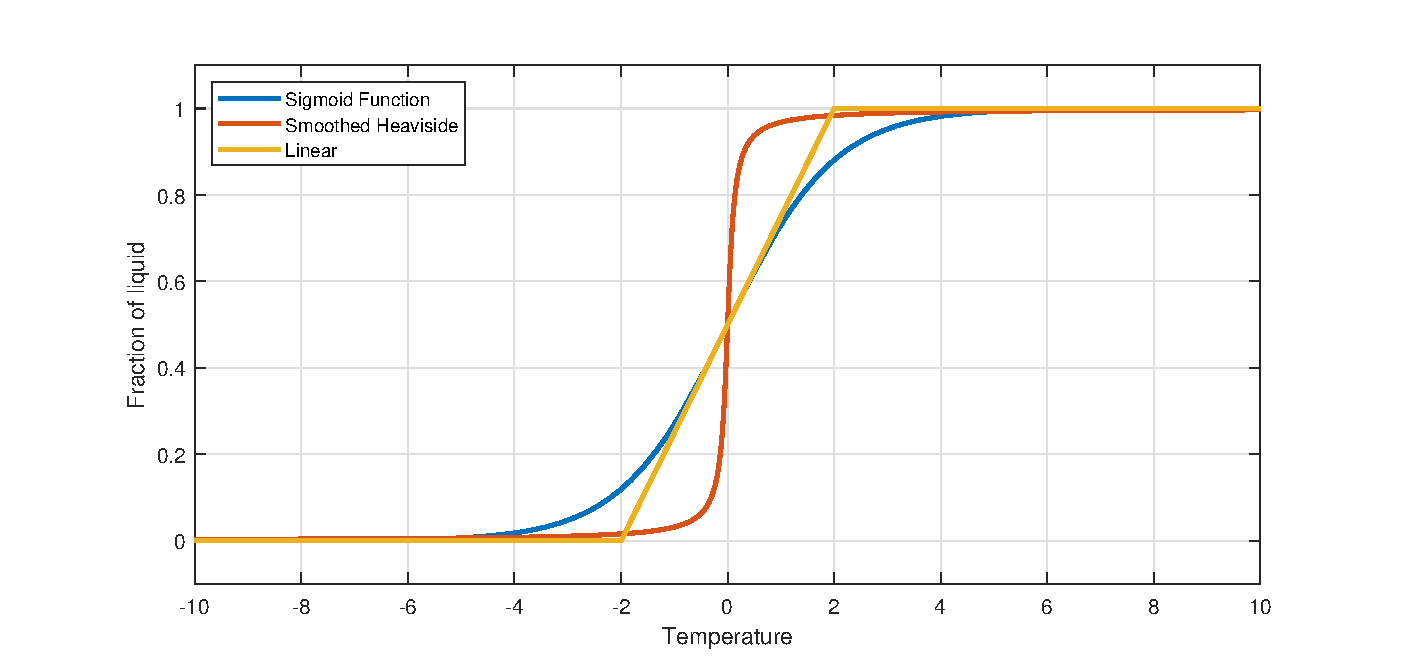
\includegraphics[width=0.9\linewidth]{figures/chapter_3/MushyZone.eps}
    \caption{Various phase transition functions}
    \label{fig:mushy_zone}
\end{figure}

The apparent heat capacity method \cite{Comini_DelGuidice_Lewis_Zienkiewicz_1974} has been utilized for this thesis. The heat capacity method works by having the heat capacity, as well as other material properties, be temperature-dependant variables, as shown in figure \ref{fig:material_properties_phase_change}. Across the mushy zone, the heat capacity jumps as a result of the latent heat of melting. The material properties can be smoothed to improve the solver's stability using the suggested functions in figure \ref{fig:mushy_zone}. The sigmoid function has been used with particular success \cite{Yang_He_2010}.
\begin{figure}[ht]
    \centering
    \includegraphics[width=0.6\linewidth]{figures/chapter_3/MaterialPropertiesOverPhaseChange.png}
    \caption{Material properties variation over phase change boundary \cite{Comini_DelGuidice_Lewis_Zienkiewicz_1974}}
    \label{fig:material_properties_phase_change}
\end{figure} 

In the apparent heat capacity method, the time-dependent heat equation shown in equation \ref{eq:time_dependant_heat_equation} is solved. Where $\rho$ is the material density, $c_{app}$ is the apparent heat capacity, and $k$ is the thermal conductivity. Some materials, such as paraffin wax have a relatively constant thermal conductivity, so for this analysis, it will be considered constant.
\begin{equation}
    \rho c_{app}(T) \frac{\partial T}{\partial t} = \nabla \cdot (k \nabla T) + q
    \label{eq:time_dependant_heat_equation}
\end{equation}

The heat capacity is defined by $c_{app}=dU/dT$ for a constant volume process, where $U$ is the internal energy. In this case, the specific internal energy $u$ is a sum of the heat capacity $c_p$ and latent heat $L$ effects \cite{Nallathambi_Specht_Bertram_2009}, as shown in equation \ref{eq:apparent_heat_capacity}.
\begin{equation}
    u = \int_{T_{ref}}^T c_p dT + L f_p
    \label{eq:apparent_heat_capacity}
\end{equation}

Equation \ref{eq:apparent_heat_capacity} introduces the phase fraction $f_p$ which can be defined in various ways, as figure \ref{fig:mushy_zone} shows. Some equations are given below in equation \ref{eq:mushy_zone}. The phase fraction ranges from zero to one and is used to track how much a material point has melted. In the equations below, the variable $a$ can control how tight the phase transition is.
\begin{subequations}
    \begin{equation}
        f_p(T) = \frac{1}{1+e^{-a(T-T_m)}}, \quad \text{Sigmoid Function}
    \end{equation}
    \begin{equation}
        f_p(T) = \lim_{a\to 0} \ \frac{1}{\pi}\tan^{-1}\left(\frac{T-T_m}{a}\right) + \frac{1}{2}, \quad \text{Smooth Heaviside}
    \end{equation}
    \begin{equation}
        f_p(T) = \begin{cases}
            0, \quad &\text{In solid phase} \\
            \frac{1}{2\Delta T}(T-T_m), &\text{In mushy zone} \\
            1, \quad &\text{In liquid phase}
        \end{cases}, \quad \text{Linear Function}
    \end{equation}
    \label{eq:mushy_zone}
\end{subequations}

Substituting the apparent heat capacity into the heat equation, the continuous description of the problem is described as shown in equation \ref{eq:continuous_phase_change_heat} \cite{Nallathambi_Specht_Bertram_2009}. In this equation, the latent heat effects are only present when the phase fraction is in the mushy zone ($0<f_p<1$). This equation is also clearly non-linear and can be severely non-linear when the latent heat effects are large, and the mushy zone is small.
\begin{equation}
    \rho\left (c_p+L\frac{\partial f_p}{\partial T} \right )\frac{\partial T}{\partial t} = k\nabla^2T + f
    \label{eq:continuous_phase_change_heat}
\end{equation}

After discretization, a discrete system of equations can be found. Equation \ref{eq:discrete_phase_change} uses the derivation by Celentano et al. \cite{Celentano_Oñate_Oller_1994} and equation \ref{eq:matrix_phase_change} gives the finite element matrices. Note that $\dot{\mathbf{L}} = \mathbf{L}^{n+1}-\mathbf{L}^n$.
\begin{subequations}
    \begin{equation}
        \mathbf{K}T + \mathbf{C}\dot{T} + \dot{\mathbf{L}} = \mathbf{F}
        \label{eq:discrete_phase_change}
    \end{equation}
    \begin{equation}
        \begin{split}
            \mathbf{K}^e&=\int_{\Omega^e}(\nabla \text{N})^T  k  \nabla \text{N} \ d\Omega^e + \int_{\Gamma}h\text{N}\text{N}^Td \ \Gamma \\
            \mathbf{C}^e&=\int_{\Omega^e}\rho c_p \text{N}\text{N}^T \ d\Omega^e \\
            \mathbf{L}^e&=\int_{\Omega^e} \text{N}\rho L f_p \ d\Omega^e \\
            \mathbf{F}^e&=\int_{\Omega^e} \text{N}\rho b \ d\Omega^e + \int_{\Gamma} \text{N}hT_{\infty} \ d\Gamma
        \end{split}
        \label{eq:matrix_phase_change}
    \end{equation}
\end{subequations}

Using backward Euler, the equation can be rewritten in the residual form shown in equation \ref{eq:residual_form_phase_change}. Taking the derivative of this gives the Jacobian shown in equation \ref{eq:jacobian_phase_change}. Note that the subscript $i$ denotes an iteration index of an iterative scheme such as Newton's method.
\begin{subequations}
    \begin{equation}
        \mathbf{R}(T^{n+1}_i)=\mathbf{F}\Delta t + \mathbf{C}T^n-(\mathbf{L}^{n+1}_i-\mathbf{L}^n)-(\mathbf{C}+\mathbf{K}\Delta t)T^{n+1}_i
        \label{eq:residual_form_phase_change}
    \end{equation}
    \begin{equation}
        \mathbf{J}(T^{n+1}_i)=-\frac{\partial \mathbf{R}}{\partial T}\Big|_i^{n+1}=\mathbf{K}\Delta t + \mathbf{C} + \frac{\partial \mathbf{L}}{\partial T}\Big|_i^{n+1}
        \label{eq:jacobian_phase_change}
    \end{equation}
\end{subequations}

An iterative scheme can then be used to determine the temperature. First, the descent direction is computed using equation \ref{eq:newton_iteration_pc}.
\begin{equation}
    \Delta T = [\mathbf{J}(T_i^{n+1})]^{-1}\mathbf{R}(T_i^{n+1})
    \label{eq:newton_iteration_pc}
\end{equation}

The descent direction can then be used in an iterative scheme such as Newton's method ($\alpha = 1$), damped Newton's method ($0<\alpha<1$), or a line search to determine a step-size $\alpha$.
\begin{equation}
    T_{i+1}^{n+1} = T_{i}^{n+1} + \alpha\Delta T
\end{equation}

\subsection*{Effective Heat Capacity Method}
The effective heat capacity method \cite{Poirier_Salcudean_1988} is another heat capacity method worth mentioning that considers the temperature distribution between the nodes in a mesh. It resolves the issue that a narrow mushy zone may occur inside the element, as illustrated in figure \ref{fig:effective_heat_capacity_method}. The left figure shows an element that would not capture the apparent heat capacity, and would essentially skip any melting effects. The right shows a node that happens to capture the apparent heat capacity, but it would overestimate its effects. This method can be used to minimize the size of the mushy zone, but as topology optimization does not require highly accurate simulations, this method has not been used and will therefore not be discussed further.
\begin{figure}[ht]
    \centering
    \includegraphics[width=.7\linewidth]{figures/chapter_3/EffectiveHeatCapacity.png}
    \caption{Heat capacity across a 1D element \cite{Poirier_Salcudean_1988}. Element failing to capture mushy-zone (left), and an element whose node captures the apparent heat capacity (right)}
    \label{fig:effective_heat_capacity_method}
\end{figure}
              \cleardoublepage    % 15-20 pages
    \chapter{Single Functional Optimization}
\label{chap:singe_functional_optimization}
Before attempting to optimize the full multi-functional problem, the single-functional problems are optimized. The approach utilized in this thesis is to use the topology optimization techniques discussed in chapter \ref{chap:topology_optimization} and apply them to the lattice structure. The lattice properties can be obtained from equations given by Bühring et al., 2022 \cite{Bühring_Soika_Schirp-Schoenen_Schröder_2022} and Soika, 2023 \cite{Piacquadio_Soika_Schirp_Schröder_Filippeschi_2023}. In the following chapters, the simple setup shown in figure \ref{fig:simple_domain} has been used. The figure shows where the thermal boundary will be (red) and where a distributed load will be defined (blue). The overall domain had a mesh generated using \emph{Gmsh} \cite{Geuzaine_Remacle_2009}, and the finite element method has been used for all simulations. Lastly, \emph{Paraview} \cite{ParaView} has been used for visualization. For this thesis, the Julia programming language has been used \cite{Julia-2017}.
\begin{figure}[ht]
  \centering
  \includegraphics[width=0.75\linewidth]{figures/chapter_4/SimpleDomain.png}
  \caption{Simple simulation setup with thermal and structural boundary conditions}
  \label{fig:simple_domain}
\end{figure}


\section{Methodology}
\subsection*{Mapping of Lattice Properties}
One of the main ideas of this thesis was to use the lattice properties directly as the material properties in the simulations. This is achieved by recognizing the relative density of the finite elements can be mapped to the porosity of the unit cells. The porosity depends on the selected cell, but generally, the porosity is a function of the cell height, strut radius, and aspect ratio. For this thesis, a fixed cell height has been used, as well as a fixed aspect ratio. Therefore, the porosity is only a function of the strut radius. As an example, the porosity of the bcc unit cell is given in equation \ref{eq:bcc_porosity} \cite{Piacquadio_Soika_Schirp_Schröder_Filippeschi_2023}.
\begin{equation}
  \epsilon = 1-2\tan^2(\Omega)\frac{r^2}{h^2}\left(\pi\frac{4}{sin(\Omega)}-\frac{16r}{3h}\left(\frac{2.993}{\sin(\pi-2\Omega)}+\frac{3.340}{\sin(\pi/2-\Omega)}\right) \right)
  \label{eq:bcc_porosity}
\end{equation}

The valid range for the unit cells porosity $\epsilon$ is typically said to be from 2.5\% to 20\%. However, the relative density $\rho$ in a topology optimization needs to range from 0\% to 100\%. Therefore a linear mapping, such as the one shown in equation \ref{eq:volfrac2porosity}, is used.
\begin{equation}
  \epsilon = \rho(\epsilon_{\text{min}}-\epsilon_{\text{max}}) + \epsilon_{\text{min}}
  \label{eq:volfrac2porosity}
\end{equation}

To determine the lattice properties, the strut radius is required. Once the required porosity is found from the relative density, the strut radius can be found quickly using a root finding method, such as those discussed in chapter \ref{chap:methods_for_optimization}.

\subsection*{Implementation}
With all the required tools implemented, the optimization methodology closely resembles that of the classical SIMP method. However, some minor adaptations have been made. The first is the use of orthotropic material properties, and the second is a slight modification of how the element sensitivities are computed.

One aspect that was proposed in this thesis was the use of automatic differentiation (AD). Automatic differentiation is a powerful tool in some scenarios, but when used for the full program, it became a performance bottleneck and provided no benefits. However, AD has been successfully used with high efficiency in two areas. The first is when computing the strut radius of the cells. To determine the strut radius, Newton's method was used which requires a gradient. The gradient can be efficiently computed using the library \emph{ForwardDiff} \cite{RevelsLubinPapamarkou2016}. Another area where the AD is very useful is for computing the finite element derivatives. Each element is a function of only the relative density, so \emph{ForwardDiff} \cite{RevelsLubinPapamarkou2016} can be efficiently used here to compute both the element matrix and its derivative. Regardless of the problem being solved, the following steps shown in figure \ref{fig:optimization_flowchart} are followed.
% \begin{enumerate}[nosep]
%   \item Define geometry and boundary conditions.
%   \item Map the relative density to porosity for each element and determine the strut radius.
%   \item Determine the lattice properties for each element from the strut radii.
%   \item Perform finite element analysis ($\mathbf{K}u=f$).
%   \item Compute element sensitivities and compute compliance.
%   \item Update element relative densities.
%   \item Repeat from step 2. until converged, or the maximum number of iterations is reached.
% \end{enumerate}
\begin{figure}[ht]
  \centering
  \includegraphics[width=0.9\linewidth]{figures/chapter_4/OptimizationFlowchart.png}
  \caption{High-level optimization flow-chart}
  \label{fig:optimization_flowchart}
\end{figure}


\section{Refinement Studies}
\subsection*{Mesh Refinement}
One problem with finite element analysis is a phenomenon known as mesh dependency. This occurs because the solution obtained using the finite element method is an approximation of a continuous domain. The finite element method discretizes the domain into elements where a set of polynomials is solved. As the elements become smaller through refinement, the approximation approaches the true solution. By comparing the results obtained on different meshes, a measure of the mesh dependency can be obtained. If the results are the same, then mesh independence is achieved, and the results are more likely to represent the true solution. 

Four mesh refinement levels have been used in the following study that have been summarised in table \ref{table:mesh_refinement_mesh_data}. The same filter radius needed to be used on each mesh as changing the filter leads to a different equation being solved, as has been mentioned in chapter \ref{chap:topology_optimization}. The porosity range for these studies was set from 0\% to 20\% to obtain clearer results.
\begin{table}[ht]
  \centering
  \begin{tabular}{c | c | c}
    & Number of elements & Element size \\ \hline
    Coarsest & 200 & 5.0mm \\ \hline
    Coarse & 800 & 2.5mm \\ \hline
    Medium & 3200 & 1.25mm \\ \hline
    Fine & 5000 & 1.0mm \\ \hline
  \end{tabular}
  \caption{Mesh data}
  \label{table:mesh_refinement_mesh_data}
\end{table}

\subsubsection*{\emph{Structural Problem}}
Just by observation, results obtained for the coarse and fine mesh, shown in figure \ref{fig:mesh_refinement_structural} for the structural problem, appear to be the same. To further ensure the results are similar, the structural compliance of each structure has been computed as shown in table \ref{table:mesh_refinement_compliance}, and the relative error w.r.t the fine mesh has been determined. 
\begin{table}[ht]
  \centering
  \begin{tabular}{c | c | c | c | c}
    Mesh Level & Coarsest & Coarse & Medium & Fine \\ \hline
    Compliance & $16.6386\times10^{-3}$ & $15.5507\times10^{-3}$ & $15.6140\times10^{-3}$ & $15.6204\times10^{-3}$ \\ \hline
    Relative Error & 6.52\% & 0.44\% & 0.04\% & - \\ \hline
  \end{tabular}
  \caption{Compliance results from mesh refinement study}
  \label{table:mesh_refinement_compliance}
\end{table}

As was mentioned, the coarse mesh already produces structures that closely resemble the fine mesh. Both structures shown in figure \ref{fig:mesh_refinement_structural} have the same features, so if the goal is to obtain a structure, without much regard for the accuracy of the simulation, the coarse mesh is already appropriate, given a large filter radius. However, using a large filter radius leads to local minima being found as will be shown in the filter radius refinement study, so a decision regarding the trade-offs needs to be made. 
\begin{figure}[ht]
  \centering
  \hfill
  \begin{subfigure}[b]{0.4\linewidth}
      \includegraphics[width=\linewidth]{figures/chapter_4/MeshRefinementCoarse.png}
      \caption{Optimized coarse mesh}
  \end{subfigure}
  \hfill
  \begin{subfigure}[b]{0.4\linewidth}
      \includegraphics[width=\linewidth]{figures/chapter_4/MeshRefinementFine.png}
      \caption{Optimized fine mesh}
  \end{subfigure}
  \hfill
  \caption{Mesh refinement study for structural problem of two mesh levels}
  \label{fig:mesh_refinement_structural}
\end{figure}

\subsubsection*{\emph{Thermal Problem}}
Once again, by observation, the results between the coarse and fine mesh appear to be pretty similar, as shown in figure \ref{fig:mesh_refinement_thermal}. To measure how similar the results are, the maximum temperature was taken for each mesh level. The results are essentially the same for each mesh level, so in this regard, any mesh could be chosen.
\begin{table}[ht]
  \centering
  \begin{tabular}{c | c | c | c | c}
    Mesh Level & Coarsest & Coarse & Medium & Fine \\ \hline
    Max Temperature [K] & $450.130$ & $450.171$ & $450.176$ & $450.176$ \\ \hline
    Relative Error & 0.010\% & 0.001\% & 0.000\% & - \\ \hline
  \end{tabular}
  \caption{Compliance results from mesh refinement study}
  \label{table:mesh_refinement_temperature}
\end{table}

A similar conclusion to the structural results can also be drawn for the thermal mesh refinement study. That being if only the generated structure is important, and the actual temperature results are not of any concern, the coarse mesh can be used.
\begin{figure}[ht]
  \centering
  \hfill
  \begin{subfigure}[b]{0.4\linewidth}
      \includegraphics[width=\linewidth]{figures/chapter_4/MeshRefinementCoarseThermal.png}
      \caption{Optimized coarse mesh}
  \end{subfigure}
  \hfill
  \begin{subfigure}[b]{0.4\linewidth}
      \includegraphics[width=\linewidth]{figures/chapter_4/MeshRefinementFineThermal.png}
      \caption{Optimized fine mesh}
  \end{subfigure}
  \hfill
  \caption{Mesh refinement study for thermal problem of two mesh levels}
  \label{fig:mesh_refinement_thermal}
\end{figure}


\subsection*{Filter Refinement Studies}
As was discussed in chapter \ref{chap:topology_optimization}, the use of a filter is a necessity in topology optimation to avoid the \emph{checkerboard problem}. Furthermore, by using a filter, a mesh-independent result can be obtained, as has already been shown in the previous subsection. One major drawback of using a filter, however, is that a different problem is being solved than the original thermal or structural problem \cite{Bendsøe_2004}. This essentially means the resulting structure depends both on the filter radius and how fine the mesh is, as a finer mesh allows a smaller filter radius to be used which in turn results in higher-resolution structures being generated.

For the filter refinement study, three filter levels were used, as well as the fine mesh which has $1mm$ elements. This means the minimum filter size is 1mm, otherwise, the filter will not intersect with any of the neighboring elements. The chosen filter radii are $5mm$, $2.5mm$ and $1.5mm$. The smallest possible filter radius should be used to minimize the number of grey elements, but also to get as close to the true structural or thermal problem as possible.

\subsubsection*{\emph{Structural Problem}}
The optimized results for the structural problem show distinctly different structures. In these structures, the sensitivities are filtered over too many elements resulting in a completely different structure. The only advantage of using the large filter radius is that mesh-independent results can be obtained for very coarse meshes. To have a measure of how different the results are, the compliance of each structure has been tabulated in table \ref{table:filter_refinement_compliance}. The relative error w.r.t the filter radius of 1.5mm is also given. The results show that the filter has a significant impact on the results.
\begin{figure}[ht]
  \centering
  \begin{subfigure}[b]{0.45\linewidth}
    \includegraphics[width=\linewidth]{figures/chapter_4/FilterRefinement5.png}
    \caption{Filter radius of 5mm}
  \end{subfigure}
  \hfill
  \begin{subfigure}[b]{0.45\linewidth}
    \includegraphics[width=\linewidth]{figures/chapter_4/FilterRefinement25.png}
    \caption{Filter radius of 2.5mm}
  \end{subfigure}
  \begin{subfigure}[b]{0.45\linewidth}
    \includegraphics[width=\linewidth]{figures/chapter_4/FilterRefinement15.png}
    \caption{Filter radius of 1.5mm}
  \end{subfigure}
  \caption{Filter refinement study for the structural problem}
  \label{fig:radius_refinement_solid}
\end{figure}

\begin{table}[ht]
  \centering
  \begin{tabular}{c | c | c | c}
    Filter Radius & 5mm & 2.5mm & 1.5mm \\ \hline
    Compliance & $17.5207\times 10^-3$ & $16.0625\times 10^-3$ & $15.8576\times 10^-3$ \\ \hline
    Relative Error & 10.49\% & 1.29\% & - \\ \hline
  \end{tabular}
  \caption{Compliance results from filter refinement study}
  \label{table:filter_refinement_compliance}
\end{table}

\subsubsection*{\emph{Thermal Problem}}
The structures obtained from the thermal topology optimization each produce six main branches, but when the filter radius is reduced, smaller branches are allowed to form. To get a measure of the difference between the results, the thermal compliance has been computed for each problem, and tabulated in table \ref{table:filter_refinement_compliance_thermal}. While these results have no real-world application, it is interesting to see that the compliance increases slightly with the coarsest mesh. The reason they have no real-world application is because the simulation has a uniform \emph{convection} throughout the domain. In reality, convection would only occur on the boundary of the branches that form. 
\begin{figure}[ht]
  \centering
  \begin{subfigure}[b]{0.45\linewidth}
    \includegraphics[width=\linewidth]{figures/chapter_4/FilterRefinementThermal5.png}
    \caption{Filter radius of 5mm}
  \end{subfigure}
  \hfill
  \begin{subfigure}[b]{0.45\linewidth}
    \includegraphics[width=\linewidth]{figures/chapter_4/FilterRefinementThermal25.png}
    \caption{Filter radius of 2.5mm}
  \end{subfigure}
  \begin{subfigure}[b]{0.45\linewidth}
    \includegraphics[width=\linewidth]{figures/chapter_4/FilterRefinementThermal15.png}
    \caption{Filter radius of 1.5mm}
  \end{subfigure}
  \caption{Filter refinement study for the thermal problem}
  \label{fig:radius_refinement_thermal}
\end{figure}

\begin{table}[ht]
  \centering
  \begin{tabular}{c | c | c | c}
    Filter Radius & 5mm & 2.5mm & 1.5mm \\ \hline
    Compliance & 1012.79 & 1012.73 & 1012.74 \\ \hline
  \end{tabular}
  \caption{Themal compliance results of filter refinement study}
  \label{table:filter_refinement_compliance_thermal}
\end{table}


\subsection*{Scaled Boundary Condition Invarience}
Recall that the compliance is computed as $c = u^Tf$, where $u$ could be the displacements or temperature vector, and $f$ is the forcing array or right-hand side of a linear system of equations. The gradient of this vector is, generally, given in equation \ref{eq:compliance_gradient_recall}.
\begin{equation}
  \frac{\partial c}{\partial \rho_e} = u_e^T\frac{\partial K_e}{\partial \rho_e}u_e
  \label{eq:compliance_gradient_recall}
\end{equation}

This gradient does not consider how much the structure deforms, only the general shape that it deforms into. That is to say, it only considers its linear deformation pattern. Therefore, to minimize compliance, only the material properties are considered. To illustrate this point, two structures have been generated with a distributed load of $1N/m$ and $100kN/m$, as shown in figure \ref{fig:force_invarience}. The generated structures show no difference.
\begin{figure}[ht]
  \centering
  \begin{subfigure}[b]{0.47\linewidth}
    \includegraphics[width=\linewidth]{figures/chapter_4/SolidOptF1.png}
    \caption{Distributed load of $1N/m$}
  \end{subfigure}
  \begin{subfigure}[b]{0.47\linewidth}
    \includegraphics[width=\linewidth]{figures/chapter_4/SolidOptF10000.png}
    \caption{Distributed load of $100kN/m$}
  \end{subfigure}
  \caption{Illustration of the scaled boundary force invarience}
  \label{fig:force_invarience}
\end{figure}

If instead non-linear properties were considered, a non-linear simulation would need to be computed. In this case, the generated structure could be different, as is shown in literature \cite{Bendsøe_2004}. This is also likely the case for the phase change problem, as the forcing array has a significant impact on how long it takes to melt the domain. For a slow process with a low heat flux, the energy storage will resemble a sensible energy storage. In such a case, the thermal conductivity might have more of an impact on the optimal structure.


\section{Structural Optimization}
The structural optimization can be implemented in essentially the same way as typical topology optimization, as discussed in chapter \ref{chap:topology_optimization}. The only big difference in terms of implementation is the use of an orthotropic material tensor, shown in equation \ref{eq:orthotropic_material_tensor}. The elastic moduli in each direction are then obtained using the functions determined by Bühring et al., \cite{Bühring_Soika_Schirp-Schoenen_Schröder_2022}. In this implementation, the orientation of the unit cells is not optimized.
\begin{equation}
  D = \begin{pmatrix} \frac{E_x}{1 - \nu_{xy}\nu_{yx}} & \frac{\nu_{xy}E_y}{1 - \nu_{xy}\nu_{yx}} & 0 \\ \frac{\nu_{xy}E_y}{1 - \nu_{xy}\nu_{yx}} & \frac{E_y}{1 - \nu_{xy}\nu_{yx}} & 0 \\ 0 & 0 & G_{xy} \end{pmatrix}
  \label{eq:orthotropic_material_tensor}
\end{equation}

In chapter \ref{chap:topology_optimization}, the OCM and GOCM methods were discussed. While this implementation only has one constraint (that being mass), the GOCM method is preferred as it has a slight performance benefit. It may also be possible to add other constraints in the future by keeping it generic. 

\subsection*{Observations}
Some results have been obtained for the structural optimization using the lattice properties. The first result, shown in figure \ref{fig:structural_opt_5to20} shows the optimized structure obtained using a porosity range of 5\% to 20\%. The structure that is obtained does not resemble a typical topology optimization result. Usually, a topology optimization produces a structure that resembles a truss. This result instead has disconnected regions of low porosity. It is important to realize that these empty regions contain cells of 5\% porosity, so in reality, each region is connected by relatively stiff cells.
\begin{figure}[ht]
  \centering
  \includegraphics[width=0.9\linewidth]{figures/chapter_4/StructuralOptLattice5to20.png}
  \caption{Optimized structure using lattice properties with a porosity of 5\% to 20\%}
  \label{fig:structural_opt_5to20}
\end{figure}

The reason for the '\emph{disconnected}' regions results from the small range in the elastic modulus. In typical topology optimization, the elastic modulus is usually set to one, and the minimum is zero. To prevent division by zero singularities, the minimum relative density is chosen to be a small number in the order of $1\times10^{-3}$. This means when a penalization value of 3 is used, the minimum value of the elastic modulus is $1\times10^{-9}$. This range of elastic modulus means that the regions of zero relative density have a negligible contribution to the stiffness of the structure. When using the lattice properties, the range of the elastic modulus is on the order of $1\times10^5$ to $1\times10^6$. In this case, the empty regions are not negligible, and contribute a significant amount of stiffness to the structure.

To validate this fact, a new structure, shown in figure \ref{fig:structure_opt_0to20}, has been generated that uses a larger range in elastic modulus. In this optimization, the porosity was varied from 0\% to 20\%, meaning the empty regions in the structure are void of any lattice material. The resulting structure resembles a typical topology optimization. At first glance, this appears to be a more reasonable result. However, it is important to keep in mind that compliance is a function of the material properties. Therefore, a different function is being minimised which should produce a slacker structure.
\begin{figure}[ht]
  \centering
  \includegraphics[width=0.9\linewidth]{figures/chapter_4/StructuralOptLattice0to20.png}
  \caption{Optimized structure using lattice properties with a porosity range of 0\% to 20\%}
  \label{fig:structure_opt_0to20}
\end{figure}

After obtaining both structures, the lattice properties were set back to the range of 5\% to 20\% and the compliance of the structure was computed. As is to be expected, the first structure shown in figure \ref{fig:structural_opt_5to20} had a lower compliance (meaning a higher stiffness). It is expected to perform better because the compliance is minimized directly considering the lattice properties. 
\begin{table}[ht]
  \centering
  \begin{tabular}{c | c | c}
    & Porosity 5\% - 20\% & Porosity 0\% - 20\% \\
    \hline
    Compliance & $9.3696\times10^{-3}$ & $9.9976\times10^{-3}$ \\
    \hline
    Maximum Displacement & 0.4950mm & 0.5313mm
  \end{tabular}
  \caption{Results comparison between different structures with different porosity range}
\end{table}

As was shown in figure \ref{fig:thermal_properties}, the lattice properties are slightly non-linear. To see whether these effects have any impact on the optimization, another structure was generated using a linear interpolation between the maximum and minimum values from the lattice. Note that for these structures, the porosity range was set from 0\% to 20\%.
\begin{figure}[ht]
  \centering
  \begin{subfigure}[b]{0.47\linewidth}
      \includegraphics[width=\linewidth]{figures/chapter_4/StructuralOptGenericOrtho.png}
      \caption{Structure generated using a linear interpolation of the lattice properties}
  \end{subfigure}
  \hfill
  \begin{subfigure}[b]{0.47\linewidth}
      \includegraphics[width=\linewidth]{figures/chapter_4/StructuralOptLattice0to20.png}
      \caption{Structure generated using the lattice properties directly}
  \end{subfigure}
  \caption{Examples of optimized domains for structural and thermal problems}
\end{figure}

The two structures only have minor differences. The displacements and compliance are also almost identical. As a result of this, the lattice properties do not have to be used directly, which could give a slight performance benefit. For this thesis, however, the lattice properties will be used directly to ensure the results are all comparable.
\begin{table}[ht]
  \centering
  \begin{tabular}{c | c | c}
    & Interpolated Structure & Lattice Properties \\
    \hline
    Compliance & $14.2887\times10^{-3}$ & $14.2702\times10^{-3}$ \\
    \hline
    Maximum Displacement & 0.7510mm & 0.7501mm
  \end{tabular}
  \caption{Results comparison between different structures with different porosity range}
\end{table}


\section{Thermal Optimization}
For the thermal topology optimization, two approaches were investigated. The first, which is used in literature, maximizes the thermal conductivity in the domain by minimizing thermal compliance. This method has been discussed in chapter \ref{chap:topology_optimization}. The second approach is to minimize the maximum temperature after a certain time has elapsed in a phase change simulation. As with the structural problem, an orthotropic material tensor, as shown in equation \ref{eq:conductivity_tensor} is required. 
\begin{equation}
  D = \begin{pmatrix}
    k_x & 0 \\ 0 & k_y
  \end{pmatrix}
  \label{eq:conductivity_tensor}
\end{equation}  

\subsection*{Maximising Thermal Conductivity}
This approach has been attempted in literature to some degree \cite{Vargas_Huitink_Iradukunda_Eddy_2020}. The main drawback with phase change materials is their low thermal conductivity, and hence low thermal diffusivity. How evenly a phase change material melts is directly related to these values. So the idea of maximizing thermal conductivity in the domain is to attempt to have the entire domain melt as evenly as possible. This should help keep the heat source at a constant temperature for a longer duration.

\subsubsection*{\emph{Observations}}
A collection of results has been obtained for the thermal topology optimization using the lattice properties. The first result, as shown in figure \ref{fig:thermal_opt_5to20}, which uses the recommended lattice porosity range, has been obtained. Much like the structural topology, the structure does not resemble typical topology optimization results. However, unlike the structural optimization result, these results are more likely to be unreasonable. This is for two reasons. The first problem with this topology optimization is that it has no consideration of the phase change problem, which is what the structures will be used for. The second reason is there are large empty regions containing only the low-conductivity PCM and low-conductivity cells. This means that when the PCM in the dark regions has fully melted, the heat has to diffuse through a low diffusivity front. This would increase the temperature gradient resulting in a high temperature at the heat source, but a domain that still has regions of solid phase.
\begin{figure}[ht]
  \centering
  \includegraphics[width=0.85\linewidth]{figures/chapter_4/ThermalOptLattice5to20.png}
  \caption{Thermal topology optimization using lattice properties with a porosity of 5\% to 20\%}
  \label{fig:thermal_opt_5to20}
\end{figure}

To test this theory, a different structure was generated. To generate this structure, different material properties were needed. To keep the results comparable, lattice properties in the range of 0\% to 20\% were used. Note that this was \emph{only} to generate a different structure, and when performing a phase change simulation, the porosity range was set back to the range 5\% to 20\%. The generated structure is shown in figure \ref{fig:thermal_opt_0to20}. As is shown, the branches in the structure reach further into the void regions. This should result in the temperature being kept more constant for longer. One slight problem with this resulting structure, however, is that there are gray regions of intermediate density. Because of the nature of the latent heat curve shown in figure \ref{fig:thermal_properties}, these elements are undesirable and may result in the PCM melting faster.

The temperature evolution plot, shown in figure \ref{fig:phase_change_lattice}, agrees with the above-discussed theory. The structure generated using a porosity range of 0\% to 5\% does rise faster, and remain constant for longer. However, because of the number of \emph{gray} elements, the total latent heat in the system is slightly lower, as shown in table \ref{table:latent_heat_available}, and is likely the cause of the slightly increased temperature at the end of the phase change simulation. However, the difference is minimal, which implies that the material distribution is still near-optimal. In this case, compared to the structural topology optimization, it is less clear which structure is \emph{'better'} because both have essentially the same final temperature. 
\begin{figure}
  \begin{subfigure}{0.45\linewidth}
    \includegraphics[width=\linewidth]{figures/chapter_4/ThermalOptLattice0to20.png}
    \caption{Thermal topology optimization using lattice properties with a porosity of 0\% to 20\%}
    \label{fig:thermal_opt_0to20}
  \end{subfigure}
  \hfill
  \begin{subfigure}{0.5\linewidth}
    \centering
    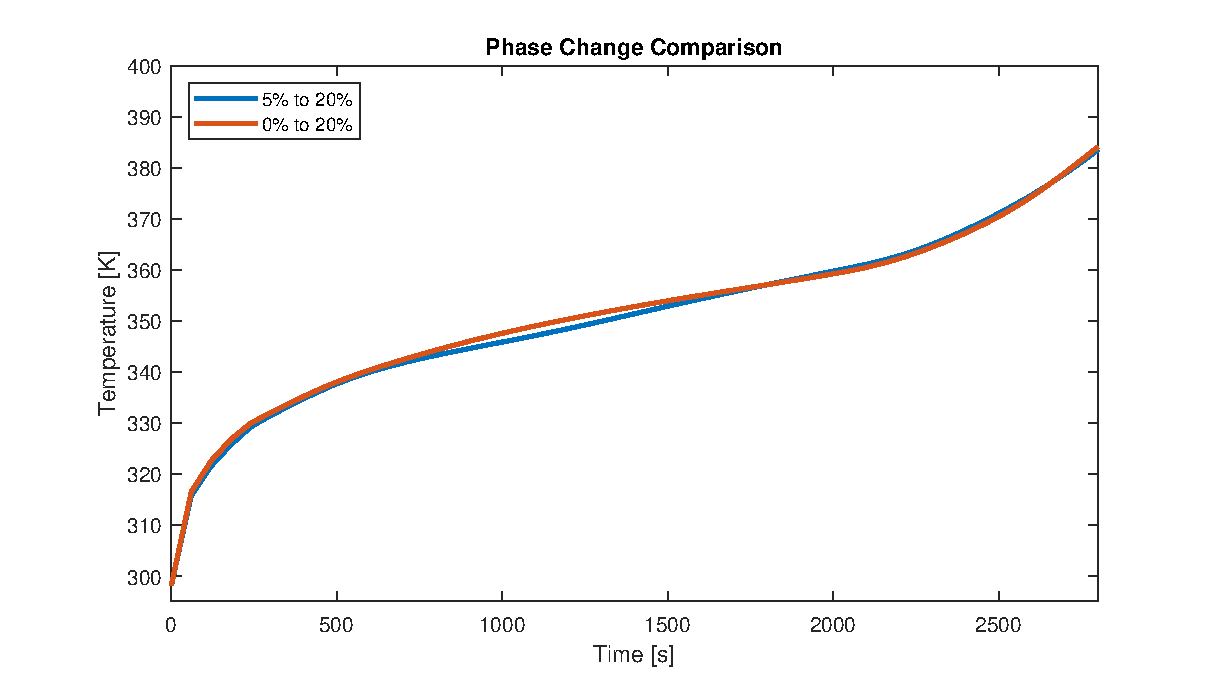
\includegraphics[width=\linewidth]{figures/chapter_4/PhaseChangeComparisonLattice.eps}
    \caption{Temperature evolution over phase change simulation}
    \label{fig:phase_change_lattice}
  \end{subfigure}
  \caption{Topology optimization results obtained using a larger porosity range (left) and the resulting phase change simulation compared to the optimal porosity range (right)}
\end{figure}
  
Another note for these structures is that the range in thermal conductivity is quite small, even when the porosity is 0\%. This is because the phase change material has a fairly high thermal conductivity compared to the maximum. This provides only a small change in the order of magnitude which is why there are minimal branches generated. To determine whether using the lattice material properties provides any benefit, a final structure has been generated that uses generic thermal conductivity in the range of zero to one. The resulting structure, shown in figure \ref{fig:thermal_opt_generic}, has many small branches as well as a lot of gray elements. As has been mentioned, these gray elements are undesirable due to the non-linear nature of the latent heat curve shown in figure \ref{fig:thermal_properties}. As a result, this structure has the lowest total latent heat.
\begin{figure}[ht]
  \centering
  \begin{subfigure}{0.45\linewidth}
    \includegraphics[width=\linewidth]{figures/chapter_4/ThermalOptGeneric.png}
    \caption{Typical thermal topology optimization using generic material properties}
    \label{fig:thermal_opt_generic}
  \end{subfigure}
  \hfill
  \begin{subfigure}{0.5\linewidth}
    \includegraphics[width=\linewidth]{figures/chapter_4/PhaseChangeComparisonLatticeGeneric.eps}
    \caption{Temperature evolution of all the optimized structures}
    \label{fig:phase_change_lattice_generic}
  \end{subfigure}
  \caption{Topology optimization results obtained using generic material properties (left) and the resulting phase change simulation compared to all other structures (right)}
\end{figure}
  
Comparing all the structures in a phase change simulation shows that the lattice properties have a significant benefit in minimizing the temperature. However, this is most likely because the total latent heat available to each system varies. Figure \ref{fig:phase_change_lattice_generic} shows that the structure generated with generic properties performs the worst right from the start. At this point, the system is conduction dominant, so it could imply that the generic properties do not capture the true conductivity well enough to optimize the system. This means that the poor placement of high porosity elements around the heat source prevents the initial heat flux from being diffused quickly through the structure. 

\begin{table}[ht]
  \centering
  \begin{tabular}{c | c | c | c}
    Structure & 5\% - 20\% Porosity & 0\% - 20\% Porosity & Generic properties \\ \hline
    Total Latent Heat [MJ] & 740.207 & 738.489 & 734.139 
  \end{tabular}
  \caption{Total available latent heat in each structure}
  \label{table:latent_heat_available}
\end{table}

To further show that the structure generated for the porosity range of 5\% to 20\% is the best option, another plot has been generated to show the phase fraction of the central node on the heat flux boundary. The plot includes the phase fraction obtained for another structure that was generated for the porosity range of 10\% to 20\%. At the time this node is melting, most of the domain is below the melting temperature, so the domain can be considered as conduction dominant. This is likely why the 5\% to 20\% structure performs the best.
\begin{figure}[ht]
  \centering
  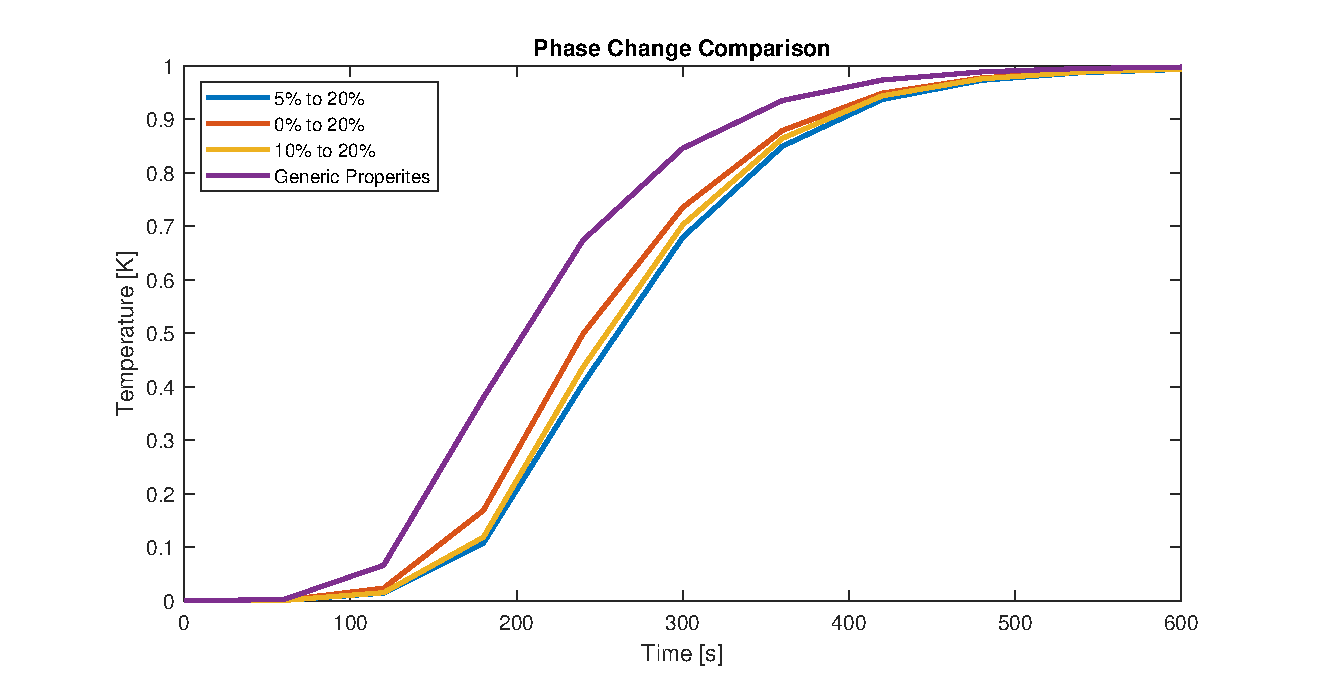
\includegraphics[width=0.7\linewidth]{figures/chapter_4/PhaseFractionRate.eps}
  \caption{Phase fraction at the hottest node in domain}
  \label{fig:phase_fraction}
\end{figure}


\subsection*{Minimising Phase Change Compliance}
This approach appears to be a novel idea where the transient effects are taken into account when finding an optimum. This would be similar to a non-linear topology optimization. The problem with this method is that there is no simple way to compute the derivative of the compliance. Recall that the compliance is defined as shown in equation \ref{eq:thermal_compliance}. However, in the transient phase change problem, the derivation of the element sensitivities can not be used. Beginning with the gradient of the compliance, shown in equation \ref{eq:compliance_gradient_pc}, a new derivation can be achieved which is given in Appendix B.
\begin{equation}
  \frac{\partial c}{\partial \rho} = \frac{\partial\mathbf{T}^T}{\partial\rho}\mathbf{f}+\mathbf{T}^T\frac{\partial\mathbf{f}}{\partial\rho}
  \label{eq:compliance_gradient_pc}
\end{equation}

The main problem with this equation is the $\frac{\partial\mathbf{T}}{\partial\rho}$ which can not be easily computed. Automatic differentiation could be used, but using the \emph{ForwardDiff} library is far too slow to be viable. The main issue is that in the forward pass, each dual variable is traced through the entire program, but most of them have no effect on the final result as the forcing vector $\mathbf{f}$ is mostly zeros. Reverse mode AD could be used instead, but because multiple Newton iterations are needed to resolve the non-linearity very high amounts of memory are required. It is for these reasons the gradient was derived, and has been computed manually.

\subsubsection*{\emph{Implementation}}
The latent heat vector and latent heat matrix can not be computed using automatic differentiation because they require the gradient of the temperature vector w.r.t the relative density. To compute them using AD would mean the entire simulation needs to be computed using AD which is what is being avoided. Here the element's relative density will be denoted using $\varphi$ to avoid confusion with the material density $\rho$. Recall that $N$ is the element shape functions, $L$ is the latent heat, and $f_{pc}$ is the phase fraction. Equation \ref{eq:latent_heat_element_gradient} shows the gradient of the element latent heat vector, and a similar gradient can be obtained for the latent heat matrix.
\begin{equation}
  \begin{split}
    L_e &= \int_{\Omega^e} N \rho(\varphi) L(\varphi)f_{pc}(\varphi)\ d\Omega^e \\
    \frac{\partial L_e}{\partial\varphi} &= \int_{\Omega^e} N \frac{\partial}{\partial\rho_e}\left(\rho(\varphi) L(\varphi)f_{pc}(T)\right)\ d\Omega^e \\
    &= \int_{\Omega^e} N \left( Lf_{pc}\frac{\partial\rho}{\partial\varphi} + \rho f_{pc}\frac{\partial L}{\partial\varphi} + \rho L\frac{\partial f_{pc}(T)}{\partial\varphi} \right) \ d\Omega^e \\
    &= \int_{\Omega^e} N \left( Lf_{pc}\frac{\partial\rho}{\partial\varphi} + \rho f_{pc}\frac{\partial L}{\partial\varphi} + \rho L\frac{\partial f_{pc}(T)}{\partial T}\frac{\partial T}{\partial\varphi} \right) \ d\Omega^e
  \end{split}
  \label{eq:latent_heat_element_gradient}
\end{equation}

Some specific implementation stages have been used in this optimization problem to obtain results as quickly as possible. Because the global matrices are assembled as a sum of the element matrices, the derivative of the matrices w.r.t any element's relative density is simply the derivative of the element matrix. This is illustrated in equation \ref{eq:phase_change_element_derivative}. These element derivatives can be efficiently computed using \emph{ForwardDiff} while computing each finite element matrix.
\begin{subequations}
  \begin{equation}
    \frac{\partial\mathbf{K}}{\partial\rho_e} = \frac{\partial\mathbf{K_e}}{\partial\rho_e}
  \end{equation}
  \begin{equation}
    \frac{\partial\mathbf{C}}{\partial\rho_e} = \frac{\partial\mathbf{C_e}}{\partial\rho_e}
  \end{equation}
  \label{eq:phase_change_element_derivative}
\end{subequations}

\subsubsection*{\emph{Observations}}
The results obtained for the phase change compliance are quite interesting because the results depend on how long the simulation runs. Three example cases have been generated. The first case runs for a longer time than required to have the domain fully melt. This essentially means the gradient is conduction-dominant. The second case only runs for as long as it takes to fully melt the domain. The third case elapses for a fixed time that does not allow the domain to fully melt.

For these structures, a coarse mesh needed to be used to produce results in a reasonable time. Even though the gradients are computed much faster, they still take at least a couple of hours to fully produce. As a result of using a coarser mesh, the filter radius had to be increased. For that reason, the results will be compared to a new pure conduction optimized structure shown in figure \ref{fig:pure_conduction_comparison}.
\begin{figure}[ht]
  \centering
  \includegraphics[width=0.8\linewidth]{figures/chapter_4/PhaseChangeCoparison.png}
  \caption{Pure conduction optimized structure}
  \label{fig:pure_conduction_comparison}
\end{figure}

The first example, which will be referred to as the conduction dominant case, is shown in figure \ref{fig:conduction_dominant_structure}. The produced structure is similar, though much softer than the pure conduction case. Very faint \emph{'ears'} are forming, similar to those that formed in the pure conduction case.
\begin{figure}[ht]
  \centering
  \includegraphics[width=0.8\linewidth]{figures/chapter_4/PhaseChangeConductionDominant.png}
  \caption{Conduction dominant structure}
  \label{fig:conduction_dominant_structure}
\end{figure}

The second example, which will be referred to as the latent heat dominant case, is shown in figure \ref{fig:latent_heat_dominant_structure}. The produced structure is much different from the previous two. In this case, the latent heat effects don't have time to be overpowered by the conduction effects. This structure contains two strong branches, which should in theory sustain a larger melting front. This means that the temperature should be held constant for a longer time.
\begin{figure}[ht]
  \centering
  \includegraphics[width=0.8\linewidth]{figures/chapter_4/PhaseChangeLatentHeatDominant.png}
  \caption{Latent heat dominant structure}
  \label{fig:latent_heat_dominant_structure}
\end{figure}

The third example, which will be referred to as the incomplete melting case, is shown in figure \ref{fig:incomplete_melting_structure}. This structure was optimized for the end time of 1800 seconds, or 30 minutes. This structure is very similar to the conduction dominant structure, except it has a larger \emph{"smoothing"} radius. This likely means the melting front is smoother, which should subject more elements to melting at once. What is obviously expected is that this structure should perform the best for the time that it was fixed, but will likely perform worse overall.
\begin{figure}[ht]
  \centering
  \includegraphics[width=0.8\linewidth]{figures/chapter_4/PhaseChangeIncompleteMelting.png}
  \caption{Incomplete melting structure}
  \label{fig:incomplete_melting_structure}
\end{figure}

To be able to compare all the structures that have been obtained, a phase change simulation has been performed for each. Figure \ref{fig:phase_change_optimal_comparison} shows the maximum temperature over time for each structure. The results are similar for each, but what is most interesting is that the pure conduction case performs the worst. The total latent heat available to that structure was the greatest of each of the examples. This highlights the fact that total latent heat does not ensure the best possible structure, but rather the placement of the \emph{grey} elements is more important. It also shows that optimizing for phase change can provide a benefit. 
\begin{figure}[ht]
  \centering
  \includegraphics[width=0.8\linewidth]{figures/chapter_4/PhaseChangePhaseChangeComparison.eps}
  \caption{Phase change simulation results}
  \label{fig:phase_change_optimal_comparison}
\end{figure}

The differences between the phase change optimal structures, on the other hand, are almost insignificant. What is most interesting, however, is that the incomplete melting case does perform best until the time it was optimized for. This is to be expected but highlights an important consideration that needs to be made if the structure is not expected to fully melt.

What is not very clear from the plot is that the latent heat dominant example does keep the temperature lower for longer, but after enough time has elapsed, the temperature rises to the same as the conduction dominant case. This result is also important, because if the goal is to keep the temperature constant for as long as possible, then a latent-heat-optimized structure should be generated. In this example, it was kept cooler for around 200 seconds longer, which could provide some benefit to some systems.

The time cost of producing the phase change optimized structures is quite significant. Many aspects of the code could be optimized and parallel computing could be implemented, but even so, for 3D structures with a fine mesh, the time to produce a structure could take many hours and would likely exceed a day.


\section{Remarks}
From the results obtained for the single functional components of this thesis, it is already clear that using lattice properties plays an important role in the kinds of structures that are produced. One can not simply neglect the lattice properties and use generic properties, as could be done for traditional topology optimization. This is because the \emph{empty} regions with a relative density of $0$ still provide a significant amount of stiffness or conduction which helps to minimize the compliance.

Based on results from both the refinement studies that were conducted, a trade-off between mesh size and filter radius needs to be reached. Using a coarse mesh produces the same structure as the finest mesh, but results in a large filter radius being required. This reduces the performance of the structure, especially in the structural problem. Using the finest mesh, however, increases the computational cost. Furthermore, high-resolution structures are produced that can not be realized in the lattice structure after homogenization. 

It is also clear that optimizing for phase change can provide some benefits. However, this benefit comes at a high computational cost that could severely limit its usability to general uses. In the future, more work needs to be done to simplify, accelerate and optimize the performance of this module to make it scalable to 3D domains.         \cleardoublepage    % 20-25 pages
    \chapter{Multi-Functional Optimization}
\label{chap:multi-functional_optimization}
With the single-functional optimization methods working, they can now be combined into a multi-functional optimization. To achieve this, the two separate functions need to be combined into a single function where an optimum can be determined. The weight method has been discussed in chapter \ref{chap:methods_for_optimization} and has been utilized for this thesis. 

Another method that could be used is the constraint method, where one function acts as a constraint on the other. However, the problem with this method is that the resulting optimal structure will satisfy one constraint, but not the other. The trade-off between the two may be too strict on the unconstrained function. Figure \ref{fig:constraint_optimal_point} shows that the constraint method can find points on the Pareto front, but they do not have a minimum error from an unobtainable utopia point. It is still possible to iterate towards the true minimum, but the weight was chosen for its elegance. 
\begin{figure}[ht]
    \centering
    \includegraphics[width=0.95\linewidth]{figures/chapter_5/ConstraintMethoLimitation.eps}
    \caption{Pareto front showing points obtained from constraint method (blue) and the real optimum (red) given an unobtainable utopia point (magenta).}
    \label{fig:constraint_optimal_point}
\end{figure}


\section{Pareto Front Generation}
As was mentioned, in this thesis, the weight method is used for generating Pareto optimal points. The sum of the weights should add to one \cite{Kochenderfer_Wheeler_2019}. The weight method converts the multiple objective functions into a single equation that can then be optimized using techniques already discussed in chapter \ref{chap:methods_for_optimization}. Equation \ref{eq:single_function_objective} shows the single objective function applied to the normalized thermal ($c^*_t$) and structural ($c^*_s$) compliance.
\begin{equation}
    J(w,\rho) = w c^*_t(\rho) + (1 - w)c^*_s(\rho)
    \label{eq:single_function_objective}
\end{equation}

To obtain reasonable results, the functions are normalized so that the compliance of each is of a similar order. This also ensures the gradients of each separate objective function are of a similar order. For the sensitivity analysis, equation \ref{eq:single_function_objective} is differentiated w.r.t the relative density, $\rho$, as shown in equation \ref{eq:single_function_objective_gradient}.
\begin{equation}
    \frac{\partial J}{\partial\rho} = w\frac{\partial c^*_t}{\partial\rho} + (1-w)\frac{\partial c^*_s}{\partial\rho}
    \label{eq:single_function_objective_gradient}
\end{equation}

With that, a Pareto front can be generated by varying the weight between 0 and 1, where the extremes would return to the single-function objective. Figure \ref{fig:mf_pareto_front_simple_domain} shows the Pareto front generated for setup shown in \ref{fig:simple_domain}. In this simulation, conductivity and stiffness were maximized for a given weight.
\begin{figure}[ht]
    \centering
    \includegraphics[width=0.6\linewidth]{figures/chapter_5/ParetoFrontForGivenStructures.eps}
    \caption{Pareto Front for Given Domain}
    \label{fig:mf_pareto_front_simple_domain}
\end{figure}

Figure \ref{fig:multi-functional_optimum_progression} shows the gradual transition from a thermal optimum to a structural optimum. The porosity range for these structures was set to 5\% to 20\%. With this range, as has already been discussed, the structures can have \emph{'disconnected'} regions, and a lack of branches and struts. These results are valid, as has already been shown in chapter \ref{chap:singe_functional_optimization}.
\begin{figure}[ht]
    \centering
    \begin{subfigure}[b]{0.45\linewidth}
        \includegraphics[width=\linewidth]{figures/chapter_5/MF_1to0.png}
        \caption{Weight of 1}
    \end{subfigure}
    \hfill
    \begin{subfigure}[b]{0.45\linewidth}
        \includegraphics[width=\linewidth]{figures/chapter_5/MF_3to1.png}
        \caption{Weight of 0.75}
    \end{subfigure}

    \centering
    \begin{subfigure}[b]{0.45\linewidth}
        \includegraphics[width=\linewidth]{figures/chapter_5/MF_1to1.png}
        \caption{Weight of 0.5}
    \end{subfigure}
    \hfill
    \begin{subfigure}[b]{0.45\linewidth}
        \includegraphics[width=\linewidth]{figures/chapter_5/MF_1to3.png}
        \caption{Weight of 0.25}
    \end{subfigure}

    \centering
    \begin{subfigure}[b]{0.45\linewidth}
        \includegraphics[width=\linewidth]{figures/chapter_5/MF_0to1.png}
        \caption{Weight of 0}
    \end{subfigure}
    \caption{The gradual progression from thermal to structural optimum obtained from the Pareto front generation}
    \label{fig:multi-functional_optimum_progression}
\end{figure}


\section{Determining Optimum Trade-off}
While the Pareto-front can be generated for a given number of weights, it is a time-consuming process that is not guaranteed to find a true optimum. Instead, a combination of methods can be used to get as close to a minimum as possible. It is important to realize that the compliance of each problem is not known without first performing a topology optimization. The shape of the Pareto front is also not known without constructing it as discussed previously. Instead, a strategy to iteratively find an optimum has been proposed in this thesis.

Assuming the Pareto-front is convex, there will be one point of minimal error. Therefore, the rate of convergence will depend on how accurate the initial guess is. To even begin to have an idea of an initial guess, the bounds of the Pareto front should be known. It is unlikely they can be determined from experience because depending on the forces, heat flux, and shape of the domain, the bounds of the Pareto front could be anything. Instead, the bounds are first determined by optimizing the single-functional problems, as has been done by Pejman and Najafi, \cite{Pejman_Najafi_2023}. This gives the range of compliance for each problem, which also allows the single-functional problems to be normalized. 

To make an educated initial guess of the optimal point, the utopia point is projected onto the line segment that can be constructed from the bounding points. Due to the shape of the Pareto front, this guess is usually quite inaccurate, but at least a rough estimate is now possible. Figure \ref{fig:optimal_point_construction} illustrates the bounding points being determined, the line segment being constructed, and the projected utopia point.
\begin{figure}[ht]
    \centering
    \includegraphics[width=0.85\linewidth]{figures/chapter_5/OptimalPointConstruction.eps}
    \caption{Initial guess (blue point) based on projecting the utopia point (magenta) onto the construction line (solid blue)}
    \label{fig:optimal_point_construction}
\end{figure}

To iterate towards the true optimum, the quadratic fit method, described by Kochenderfer, et al., \cite{Kochenderfer_Wheeler_2019} has been utilized. This method is a gradient-free bracketing method that uses information from three points to construct a parabola and then finds its minimum.
\begin{figure}[ht]
    \centering
    \includegraphics[width=0.85\linewidth]{figures/chapter_5/QuadraticFitConvergence.eps}
    \caption{Quadratic fit convergence showing the real error norm (solid blue) and the fitted parabolas (dashed red) constructed by three points (red star)}
    \label{fig:quadratic_fit_method}
\end{figure}

It turns out that generally the error measure very roughly resembles a parabola, so this method can find the true optimal point, given a reasonable tolerance, in very few iterations. This method works by updating the bounds of the parabola each iteration, and will eventually collapse around the optimal point. Figure \ref{fig:quadratic_fit_method} shows how this method converges toward the optimal point. The convergence plot shows that it is already near the optimal point after three iterations, and after five iterations the optimal point is already determined within a low tolerance. 

\subsection*{Limitations}
This method does have some drawbacks. When the optimal point is, or is near the bounding points, a couple of problems can arise. Figure \ref{fig:optimal_point_is_bounding_point} illustrates when this problem can arise. The first problem is that the projection method that is used means the initial guess may be outside the allowable weight range. To solve this issue, the initial guess can be limited to a range such as $w_\text{guess} \in [0.1, 0.9]$. The quadratic fit method can then continue as normal.

The second issue with having the optimal point near the bounding points is that the quadratic fit method might find a minimum that is outside the allowable weight range. To overcome this issue, a bisection is performed instead to update the central point in the parabola. This can be repeated until the method converges to the true optimum, or until the quadratic fit method finds a valid optimal point. Note that the weight range can not be limited for this case, because the optimum could be the bounding point.

\begin{figure}[ht]
    \centering
    \includegraphics[width=0.9\linewidth]{figures/chapter_5/BoundingPointOptimum.eps}
    \caption{Limitation where the bounding point is the optimal point}
    \label{fig:optimal_point_is_bounding_point}
\end{figure}

Another limitation is that many local minima could be present when the function is concave. In such a situation, a more accurate initial guess is required to ensure it converges to the correct minimum. Through some experimentation, however, the Pareto front is usually convex. This is because the two functions tend to contribute to each other, rather than compete.


\section{Maximizing Thermal Conductivity and Stiffness}
The algorithms developed in chapter \ref{chap:singe_functional_optimization} were for the minimization of thermal and structural compliance, as well as the minimization of phase-change compliance. This section discusses results obtained using the minimization of thermal and structural compliance.

\subsection*{Test Case 1}
To illustrate the effectiveness of the selected method, two test cases have been produced for the same Pareto front. The first utopia point was set to $U(1012.66, 0.011)$. The bounds of the Pareto front a then determined, and the compliances are normalised. The optimal point is then iteratively determined. This case converges to a reasonable tolerance in three iterations.
\begin{figure}[ht]
    \centering
    \includegraphics[width=0.8\linewidth]{figures/chapter_5/ParetoOpt_w0063.eps}
    \caption{Optimum obtained (red) for utopia point $U(1012.66, 0.011)$ (magenta)}
    \label{fig:utopia_66_011}
\end{figure}

Figure \ref{fig:optimal_structure_1} shows the structure that was generated. Compared to figure \ref{fig:multi-functional_optimum_progression}, this structure lies somewhere between structures b and c as is expected. 
\begin{figure}[ht]
    \centering
    \includegraphics[width=0.7\linewidth]{figures/chapter_5/ParetoOptimuim_Test1.png}
    \caption{Pareto-optimal structure obtained for utopia point $U(1012.66, 0.011)$}
    \label{fig:optimal_structure_1}
\end{figure}


\subsection*{Test Case 2}
In this test case, the utopia point was set to $U(1012.64, 0.014)$. This case has a much sharper error norm but still converges to the optimal point in very few iterations. The optimal point is determined with a coarse tolerance in only six iterations, and to a high resolution in nine.
\begin{figure}[ht]
    \centering
    \includegraphics[width=0.8\linewidth]{figures/chapter_5/ParetoOpt_w00854.eps}
    \caption{Optimum obtained (red) for utopia point $U(1012.64, 0.014)$ (magenta)}
    \label{fig:utopia_64_014}
\end{figure}

Figure \ref{fig:optimal_structure_2} shows the structure generated. This structure lies between structures a and b which is expected. 
\begin{figure}[ht]
    \centering
    \includegraphics[width=0.7\linewidth]{figures/chapter_5/ParetoOptimuim_Test2.png}
    \caption{Pareto-optimal structure obtained for utopia point $U(1012.64,0.014)$}
    \label{fig:optimal_structure_2}
\end{figure}

The two test cases that have been used for the simple domain show that an optimum can be found. Both optimal structures were found in only a few iterations. However, to ensure generability, more test cases have been produced with different boundary conditions in chapter \ref{chap:test_cases}.


\section{Minimising Temperature and Maximising Stiffness}
This section discusses results obtained where the phase-change compliance and structural compliance were objective functions. This section expands on observations made in chapter \ref{chap:singe_functional_optimization} where the phase change compliance optimization provided some benefits. Unfortunately, to generate a Pareto front in a reasonable amount of time, the coarsest mesh had to be used. This makes it difficult to compare results with the previous section, but the overall structure is still visible.

Figure \ref{fig:multi-functional_pc_progression} shows some of the intermediate structures that have been generated using the Pareto front generation tool. These structures were optimized until the time the domain fully melted, as this provided the most benefit as shown in figure \ref{fig:phase_change_optimal_comparison}. The progression from thermal to structural optimum is clear. Because of the chosen end time, the thermal optimum has two branches that fill much of the domain.
\begin{figure}[ht]
    \centering
    \begin{subfigure}[b]{0.45\linewidth}
        \includegraphics[width=\linewidth]{figures/chapter_5/PC_MF_1to0.png}
        \caption{Weight of 1}
    \end{subfigure}
    \hfill
    \begin{subfigure}[b]{0.45\linewidth}
        \includegraphics[width=\linewidth]{figures/chapter_5/PC_MF_3to1.png}
        \caption{Weight of 0.75}
    \end{subfigure}
    
    \begin{subfigure}[b]{0.45\linewidth}
        \includegraphics[width=\linewidth]{figures/chapter_5/PC_MF_1to1.png}
        \caption{Weight of 0.5}
    \end{subfigure}
    \hfill
    \begin{subfigure}[b]{0.45\linewidth}
        \includegraphics[width=\linewidth]{figures/chapter_5/PC_MF_1to3.png}
        \caption{Weight of 0.25}
    \end{subfigure}
    
    \begin{subfigure}[b]{0.45\linewidth}
        \includegraphics[width=\linewidth]{figures/chapter_5/PC_MF_0to1.png}
        \caption{Weight of 0}
    \end{subfigure}
    \caption{The gradual progression from phase-change to structural optimum from the Pareto front generation}
    \label{fig:multi-functional_pc_progression}
\end{figure}

To compare the results to the conductivity optimal structures, a new set of structures was generated for the former case, and the phase change results have been plotted in figure \ref{fig:phase_change_results_coarsest}. This plot shows different weight ratios. The plot shows that the weight has a much less linear relationship with the phase-change optimizer than with the conductivity optimizer. These results shown in the plot are therefore not directly relatable, but they do show that the limits in optimums are comparable.
\begin{figure}[ht]
    \centering
    \includegraphics[width=0.7\linewidth]{figures/chapter_5/PhaseChangeResultsCoarsest.eps}
    \caption{Phase change results showing the maximum temperature in the domain for the maximization of thermal conductivity and stiffness (TS/solid lines), and optimization of phase change compliance and stiffness (PS/dashed lines)}
    \label{fig:phase_change_results_coarsest}
\end{figure}

\subsection*{Test Case}
Finally, a Pareto optimal structure has been generated for the utopia point $U(212500, 0.012)$. As has been discussed, first the bounds of the Pareto front are determined, the compliances are normalized, and the optimal point is iteratively determined. The algorithm returned in six iterations but with relatively poor accuracy.
\begin{figure}[ht]
    \centering
    \includegraphics[width=0.8\linewidth]{figures/chapter_5/ParetoOpt_PC.eps}
    \caption{Optimum obtained (red) for utopia point $U(212500,0.012)$ (magenta)}
    \label{fig:pareto_optimum_phase_change}
\end{figure}

Figure \ref{fig:pareto_optimal_structure_pc} shows the structure that is obtained. It resembles a structure between figure \ref{fig:multi-functional_pc_progression} b and c. This is expected because the optimal weight is found to be around $w=0.56$.
\begin{figure}[ht]
    \centering
    \includegraphics[width=0.6\linewidth]{figures/chapter_5/ParetoOptimum_PhaseChange.png}
    \caption{Pareto-optimal structure obtained for utopia point $U(212500,0.012)$}
    \label{fig:pareto_optimal_structure_pc}
\end{figure}


\section{Remarks}
While the phase-change-structural optimization algorithm does provide a small benefit, the computational costs make it prohibitive to use more extensively. One of the major limiting factors is that the mesh needs to be quite coarse to obtain a structure in a reasonable amount of time. As the benefit is so negligible, in the following chapter, only structures obtained for the maximization of thermal conductivity and stiffness will be generated.

As was mentioned in this thesis, de-homogenization was not a major focus of this thesis because the types of cells were already defined. To illustrate a basic de-homogenization of the structure, figure \ref{fig:dehomogenized_optimal_pc_structure}. This structure is simple to generate because the positions and radius of each unit cell are determined by the mesh. This figure also helps to illustrate that the empty regions in the relative density plot are actually populated by high-porosity unit cells.
\begin{figure}[ht]
    \centering
    \includegraphics[width=0.7\linewidth]{figures/chapter_5/BasicDehomogenization.eps}
    \caption{Basic de-homogenization of structure shown in figure \ref{fig:pareto_optimal_structure_pc}}
    \label{fig:dehomogenized_optimal_pc_structure}
\end{figure}  \cleardoublepage    % 15 pages
    \chapter{Results}
\label{chap:test_cases}
Three further test cases have been produced to ensure the solver is general enough to solve a variety of different problems. Generally, the domain for spacecraft systems will be rectangular, so the same overall domain has been used. Just the position of the boundary conditions has been altered.

Each test case has a generated Pareto front for thermal and structural compliance. A Pareto optimal point is then found for each test case and is compared to the Pareto front to ensure it is reasonable. 

\section{Case One}
Test case one has been designed to attempt to have two competing objective functions. The idea is that material needs to be distributed to the top and bottom of the domain which should take away from each objective. Figure \ref{fig:test_case_one_domain} shows the domain with the two boundary conditions.
\begin{figure}[ht]
    \centering
    \includegraphics[width=0.8\linewidth]{figures/chapter_6/Case1Domain.png}
    \caption{Test Case One Domain with a thermal load (red) and structural load (blue)}
    \label{fig:test_case_one_domain}
\end{figure}

Figure \ref{fig:test_case_one_pareto_front} shows the obtained Pareto front for this setup. Despite the fact that the two boundary conditions were intended to be competing, it turns out they contribute to each other, as is observed in the Pareto front for the weights between $w=0.25$ to $w=0.75$ are close to each other.
\begin{figure}[ht]
    \centering
    \includegraphics[width=0.6\linewidth]{figures/chapter_6/Case2_ParetoFront.eps} 
    \caption{Pareto front for test case one showing the chosen utopia point (magenta)}
    \label{fig:test_case_one_pareto_front}
\end{figure}

Figure \ref{fig:test_case_one_structures} shows some optimal structures that were recorded. The structure optimized for a weight of $w=0.5$ shows that although the boundary conditions are not aligned, the generated structure produces a shape that allows the two boundary conditions to assist each other in minimizing the total objective function.
\begin{figure}[ht]
    \begin{subfigure}[b]{0.3\linewidth}
        \includegraphics[width=\linewidth]{figures/chapter_6/Case2_MF_0to1.png}
        \caption{Optimized structure for \\$w=0.0$}
    \end{subfigure}
    \hfill
    \begin{subfigure}[b]{0.3\linewidth}
        \includegraphics[width=\linewidth]{figures/chapter_6/Case2_MF_1to1.png}
        \caption{Optimized structure for \\$w=0.5$}
    \end{subfigure}
    \hfill
    \begin{subfigure}[b]{0.3\linewidth}
        \includegraphics[width=\linewidth]{figures/chapter_6/Case2_MF_1to0.png}
        \caption{Optimized structure for \\$w=1.0$}
    \end{subfigure}
    \caption{Optimized structures for test case one}
    \label{fig:test_case_one_structures}
\end{figure}

Figure \ref{fig:test_case_one_pareto_optimum} shows the Pareto optimal point determined for the utopia point $U(312.6,0.01)$. Under these boundary conditions, the developed algorithm had no issues converging to the selected utopia point, even though the error norm plot has quite a wide well. The optimal point was found in just two iterations due to the initial guess being so accurate.
\begin{figure}[ht]
    \centering
    \hfill
    \begin{subfigure}[b]{0.45\linewidth}
        \includegraphics[width=\linewidth]{figures/chapter_6/Case1_ParetoOptimum.png}
        \caption{Pareto optimal structure}
    \end{subfigure}
    \hfill
    \begin{subfigure}[b]{0.25\linewidth}
        \includegraphics[width=\linewidth]{figures/chapter_6/Case1_ErrorNormPlot.eps}
        \caption{Error norm plot}
    \end{subfigure}
    \hfill
    \caption{Optimal structure obtained for utopia point $U(312.6,0.01)$ (left) as well as the error norm plot (right) produced for verification}
    \label{fig:test_case_one_pareto_optimum}
\end{figure}


\section{Case Two}
Test case two has been designed to test different boundary conditions. The bottom left node is fixed, while the bottom right node can slide in the x direction. A large distributed load across the top of the domain is also used. The thermal boundary condition is placed along the bottom in the center, meaning these boundary conditions should contribute to each other for the overall goal function.
\begin{figure}[ht]
    \centering
    \includegraphics[width=0.8\linewidth]{figures/chapter_6/Case2Domain.png}
    \caption{Test Case Two Domain}
    \label{fig:test_case_two_domain}
\end{figure}

Figure \ref{fig:test_case_two_pareto_front} shows the Pareto front obtained for the boundary conditions of this case. It turns out that the boundary conditions partially compete with each other, unlike what was hypothesized. This occurs because as the thermal optimum develops, it removes a significant amount of material from where it is needed for the structural optimum. 
\begin{figure}[ht]
    \centering
    \includegraphics[width=0.6\linewidth]{figures/chapter_6/Case1_ParetoFront.eps} 
    \caption{Pareto front for test case two showing the chosen utopia point (magenta)}
    \label{fig:test_case_two_pareto_front}
\end{figure}

Figure \ref{fig:test_case_two_structures} also shows some optimal structures that were generated. They show that the thermal optimum essentially grows from the structural optimum. This backs up the idea that the two boundary conditions contribute to each other.
\begin{figure}[ht]
    \begin{subfigure}[b]{0.3\linewidth}
        \includegraphics[width=\linewidth]{figures/chapter_6/Case1_MF_0to1.png}
        \caption{Optimized structure for \\$w=0.0$}
    \end{subfigure}
    \hfill
    \begin{subfigure}[b]{0.3\linewidth}
        \includegraphics[width=\linewidth]{figures/chapter_6/Case1_MF_1to1.png}
        \caption{Optimized structure for \\$w=0.5$}
    \end{subfigure}
    \hfill
    \begin{subfigure}[b]{0.3\linewidth}
        \includegraphics[width=\linewidth]{figures/chapter_6/Case1_MF_1to0.png}
        \caption{Optimized structure for \\$w=1.0$}
    \end{subfigure}
    \caption{Optimized structures for test case two}
    \label{fig:test_case_two_structures}
\end{figure}

Figure \ref{fig:test_case_two_pareto_optimum} shows the optimized structure and error norm plot. Again, the minimum error is found quite easily due to a sharpening towards the optimum. Even though these are simple boundary conditions, this result in particular shows that error and Pareto front aren't always going to produce results that are expected. This test case also shows that the boundary conditions that should contribute to each other can end up competing when they are too far apart. Too much material is required by each separate function which results in one function, in this case, the thermal function, dominating the kind of structure that can form. The optimum was determined within a good tolerance in five iterations but fully converged in nine.
\begin{figure}[ht]
    \centering
    \hfill
    \begin{subfigure}[b]{0.45\linewidth}
        \includegraphics[width=\linewidth]{figures/chapter_6/Case2_ParetoOptimum.png}
        \caption{Pareto optimal structure}
    \end{subfigure}
    \hfill
    \begin{subfigure}[b]{0.25\linewidth}
        \includegraphics[width=\linewidth]{figures/chapter_6/Case2_ErrorNormPlot.eps}
        \caption{Error norm plot}
    \end{subfigure}
    \hfill
    \caption{Optimal structure obtained for utopia point $U(312.6,0.01)$ (left) as well as the error norm plot (right) produced for verification}
    \label{fig:test_case_two_pareto_optimum}
\end{figure}


\section{Case Three}
Test case three has been designed as an extension to test case two to ensure that expected results are obtained for asymmetric boundary conditions. Based on the results from test cases one and two, it is expected that the boundary conditions contribute to each other than in case two. This is because they already partially contribute, but in this case, the material can be distributed closer to each boundary condition so that neither function can be dominant.
\begin{figure}[ht]
    \centering
    \includegraphics[width=0.7\linewidth]{figures/chapter_6/Case3Domain.png}
    \caption{Test Case Three Domain}
    \label{fig:test_case_three_domain}
\end{figure}

Figure \ref{fig:test_case_three_pareto_front} shows the Pareto front obtained for this final test case. Again the weights between $w=0.25$ and $w=0.75$ are close to each other because, as mentioned in this section's opening, the two boundary conditions contribute to each other. In fact, these two boundary conditions contribute so well with each other that between the weights $w=0.0$ to $w=0.25$ and $w=0.75$ to $w=1.0$, weakly Pareto optimal points are essentially found.
\begin{figure}[ht]
    \centering
    \includegraphics[width=0.6\linewidth]{figures/chapter_6/Case3_ParetoFront.eps} 
    \caption{Pareto front for test case three showing the chosen utopia point (magenta)}
    \label{fig:test_case_three_pareto_front}
\end{figure}

Figure \ref{fig:test_case_three_structures} shows how the two boundary conditions contribute to each other, especially on the right-hand side of the domain. They contribute because the thermal boundary condition allows the material to remain where it is required by the structural optimum on the right of the domain. This contrasts with case 2 which uniformly removed material from the top of the domain, limiting the structural compliance.
\begin{figure}
    \begin{subfigure}[b]{0.3\linewidth}
        \includegraphics[width=\linewidth]{figures/chapter_6/Case3_MF_0to1.png}
        \caption{Optimized structure for \\$w=0.0$}
    \end{subfigure}
    \hfill
    \begin{subfigure}[b]{0.3\linewidth}
        \includegraphics[width=\linewidth]{figures/chapter_6/Case3_MF_1to1.png}
        \caption{Optimized structure for \\$w=0.5$}
    \end{subfigure}
    \hfill
    \begin{subfigure}[b]{0.3\linewidth}
        \includegraphics[width=\linewidth]{figures/chapter_6/Case3_MF_1to0.png}
        \caption{Optimized structure for \\$w=1.0$}
    \end{subfigure}
    \caption{Optmized structures for test case three}
    \label{fig:test_case_three_structures}
\end{figure}

Figure \ref{fig:test_case_three_pareto_optimum} shows the optimized structure and error norm plot. In this case, the minimum is close, but not exactly the minimum. The initial guess was good, but the algorithm converged too slowly. The error is still within a reasonable tolerance, but improvements should be made to ensure a true global minimum can be found.
\begin{figure}[ht]
    \centering
    \hfill
    \begin{subfigure}[b]{0.5\linewidth}
        \includegraphics[width=\linewidth]{figures/chapter_6/Case3_ParetoOptimum.png}
        \caption{Pareto optimal structure}
    \end{subfigure}
    \hfill
    \begin{subfigure}[b]{0.3\linewidth}
        \includegraphics[width=\linewidth]{figures/chapter_6/Case3_ErrorNormPlot.eps}
        \caption{Error norm plot}
    \end{subfigure}
    \hfill
    \caption{Optimal structure obtained for utopia point $U(312.6,0.01)$ (left) as well as the error norm plot (right) produced for verification}
    \label{fig:test_case_three_pareto_optimum}
\end{figure}


\section{Remarks}
Of the boundary conditions that were devised, all produced a convex Pareto-front. As the algorithm is sensitive to the initial guess, this information can be useful when trying to determine the initial weight. Instead of projecting the point onto a line segment, the point could instead be projected onto the reciprocal function $y=k/x$, where $k$ can be used to control how sharp the shape of the curve is. The most generic form of this function is given in equation \ref{eq:recipricol_function_generic}.
\begin{equation}
    y = \frac{k}{x+a} + b
    \label{eq:recipricol_function_generic}
\end{equation}

The variables $a$ and $b$ are used to shift the function. They can be determined by solving a pair of simultaneous equations. If $y$ is the normalized compliance of the first function, and $x$ for the second, then a system of simultaneous can be determined as shown in equation \ref{eq:recipicol_simultaneous_equations}.
\begin{equation}
    \begin{split}
        \frac{k}{a} + b &= 1 \\
        \frac{k}{1 + a} + b &= 0
    \end{split}
    \label{eq:recipicol_simultaneous_equations}
\end{equation}

By rearranging the second equation, an equation for $b$ can be found which can then be used to determine $a$ using the quadratic formula, as shown in equation \ref{eq:recipicol_solved}.
\begin{equation}
    \begin{split}
        b &= \frac{k}{1 + a} \\
        a &= \frac{-1 + \sqrt{1 + 4k}}{2}
    \end{split}
    \label{eq:recipicol_solved}
\end{equation}

With that, the utopia point, $U$, can be projected onto the curve by defining the goal function shown in equation \ref{eq:goal_function}. The value $x$ can be determined using a gradient descent or similar method.
\begin{equation}
    \text{argmin}_{x\in[0,1]} \lVert (y,x) - U\rVert _p
    \label{eq:goal_function}
\end{equation}

\begin{figure}[ht]
    \centering
    \includegraphics[width=0.5\linewidth]{figures/chapter_6/ProjectionIdea.eps}
    \caption{Projection (blue) of utopia point (magenta) onto the reciprocal function (blue line)}
\end{figure}

Once $x$ has been determined, the distance along the curve from $x=0$ needs to be determined. It is this distance that corresponds to the weight. This can be found by solving equation \ref{eq:distance_along_curve}. This method assumes the weights to be even distributed along the curve, which is generally not the case. This approach could be modified with a weighting function to reduce the calculated \emph{distance} along the curve near the endpoints.
\begin{equation}
    S(x) = \frac{1}{S(1)} \int_0^x \sqrt{(1 + \left(\frac{dy}{dx}\right)^2)} \ dt 
    \label{eq:distance_along_curve}
\end{equation}

To resolve the issue discussed in case 3, the quadratic fit method could be accelerated by considering gradient information obtained by previous iterations. A gradient descent sub-step could be performed to improve convergence in shallow wells. However, certain checks would need to be performed to ensure minimal overshooting occurs.                       \cleardoublepage    % 5 pages
    \chapter{Conclusion}
\label{chap:conclusion}
\section{Conclusion}
In this thesis, a methodology to produce multi-functional topology-optimized structures has been developed and investigated. Structural, thermal and phase change considerations have been incorporated, and the results they produce have been discussed. While this thesis focussed on their use in spacecraft structures, the methodology can also be applied to Earth-bound systems.

The thesis began by looking into the theoretical background of all the ingredients required. Heat transfer and the Stefan problem were the roots of what would be built on. Structural mechanics was also the most important topic that was required to produce traditional topology-optimized structures. Finally, optimization methods were discussed which would be used throughout this thesis. While automatic differentiation was not as useful as hoped, it was implemented in many stages for computing certain gradients efficiently.

The state of the art was then researched which would provide the groundwork for what this thesis would build on. Homogenized properties for the cellular structures were provided that were used in all topology optimizations. Latent heat energy storage materials were found, and paraffin was selected for this thesis as it was a simple material to implement that could be widely varied for specific use cases. Topology optimization algorithms were found, most importantly the structural and thermal algorithms. Multifunctional topology optimization methods were found in the literature that could be adapted to this specific case.

Finally, a methodology for the structural-thermal and structural-phase-change optimization has been developed. The algorithms are so general that they can be applied to any material or any homogenized unit cell. Automatic differentiation, while not useful for solving the full script, was extremely useful and efficient in computing element matrices and simple program derivatives. Some test cases were also investigated to ensure different boundary conditions could be solved.

\section{Discussion}
While This thesis developed and investigated a methodology for multi-functional optimization, it did not explicitly consider the de-homogenization of the produced structure. The structures that are produced contain elements much smaller than a unit cell. This means that their reactive density needs to be somehow averaged over the volume of a unit cell in a de-homogenization process. This will naturally produce a different stiffness and maximum temperature.

This thesis was also focused on space-craft structures. This means the phase change simulation only considers conduction and no convection. Topology optimization has been successfully performed considering the Navier-Stokes equations \cite{Alexandersen_Sigmund_Aage_2016}, but this time cost is significant. In future work, phase change optimized structures should consider convection to be able to produce highly optimized structures for use on Earth. Such structures could be used for energy storage as a low-cost and efficient alternative to chemical batteries.                    \cleardoublepage    % 3 page

% References
\addcontentsline{toc}{chapter}{Literatur}
\nocite{*} 
\bibliographystyle{ieeetr}
\bibliography{references}               \cleardoublepage

% Appendices
\appendix
\pagestyle{scrheadings}
    \chapter{Lattice Properties}
\label{appendix:A}

The properties provided here have been obtained for the $bcc$ and $f_2cc,z$ unit cells. The properties have been obtained by Soika \cite{Piacquadio_Soika_Schirp_Schröder_Filippeschi_2023} and Bühring, et al., \cite{Bühring_Soika_Schirp-Schoenen_Schröder_2022}.

Where for the thermal properties: \\
$\epsilon$ is the cell porosity. \\
$r$ is the strut radius.\\
$h$ is the cell height.\\
$R_i$ is the thermal resistance for different regions.\\
$k_s$ is the thermal conductivity of the solid material. \\
$k_f$ is the thermal conductivity of the phase change material. \\
$k_i$ is the effective thermal conductivity in each basis direction.

Where for the structural properties: \\
$E$ is Young's modulus of the lattice material. \\
$E_i$ is the effective Young's modulus in each basis direction. \\
$r$ is the strut radius. \\
$h$ is the cell height. \\
$\omega$ is the cell strut incliniation.

The properties follow on the next page.

\vfill \pagebreak
\section*{$bcc$ Unit Cell}
\subsection*{Thermal Properties}
\begin{equation*}
    \begin{split}
        \Omega &= \arctan\left(\frac{\tan(\omega)}{\sqrt{2}}\right) \\
        \epsilon &= 1 - 2\tan^2(\Omega)\frac{r^2}{h^2}\left[ \pi\frac{4}{\sin(\Omega)}-\frac{16r}{3h}\left(\frac{2.993}{\sin(\pi-2\Omega)}+\frac{3.340}{\sin(\pi/2-\Omega)}\right) \right] \\
        V_4 &= 2\frac{16}{3\sin(\pi-2\Omega)}r^3-12\left(\sqrt{8}-\sqrt{6}\right)r^3
    \end{split}
\end{equation*}
\begin{table}[ht]
    \centering
    \begin{tabular}{c | c}
        $1,2$ Direction & $3$ Direction \\ \hline
        \parbox{0.49\linewidth}{
        \begin{equation*}
            \begin{split}
                t_4 &= \left(V_4\sin(\Omega)\cos^2(\Omega)\right)^{1/3} \\
                a &= \sqrt{\frac{2}{\cos^2(\Omega)}+\frac{1}{\sin^2(\Omega)}} \\
                L_\text{str} &= \frac{h}{2\sin(\Omega)}-at_4 \\
                R_1 = R_3 &= \frac{2\cos^2(\Omega)}{4.277\sin(\Omega)t_4k_s} \\
                R_2 &= \frac{L\text{str}}{\pi r^2k_s} \\
                R_\text{str} &= 2(R_1 + R_2 + R_3) \\
                R_s &= \frac{R_\text{str}}{4} \\
                k_{1,2} &= \epsilon k_f + \frac{1}{hR_s}
            \end{split}
        \end{equation*} 
        }
        & 
        \parbox{0.49\linewidth}{
        \begin{equation*}
            \begin{split}
                t_4 &= \left(V_4\sin^2(\Omega)\cos(\Omega)\right)^{1/3} \\
                a &= \sqrt{\frac{1}{\cos^2(\Omega)}+\frac{2}{\sin^2(\Omega)}} \\
                L_\text{str} &= \frac{h}{2\sin(\Omega)}-at_4 \\
                R_1 = R_3 &= \frac{2\sin^2(\Omega)}{1.903\cos(\Omega)t_4k_s} \\
                R_2 &= \frac{L\text{str}}{\pi r^2k_s} \\
                R_\text{str} &= 2(R_1 + R_2 + R_3) \\
                R_s &= \frac{R_\text{str}}{4} \\
                k_{1,2} &= \epsilon k_f + \frac{2\tan^2(\Omega)}{hR_s}
            \end{split}
        \end{equation*} 
        }
    \end{tabular}
\end{table}


\subsection*{Structural Prorperties}
\begin{equation*}
    \begin{split}
        E_{1,2} &=\frac{2\sqrt{2}\pi Er^2}{h^2}\left[ 1 + 12\frac{r^2}{h^2}\left(\sin^2(\omega)+1\right)\tan^2(\omega) \right]\times sin^2(\omega)\cos(\omega) \\
        E_3 &=\frac{8\pi Er^2}{h^2}\left[ 1 + 12\frac{r^2}{h^2}\cos^2(\omega) \right]\times \sin^3(\omega)\tan^2(\omega)
    \end{split}
\end{equation*}
    

\vfill \pagebreak
\section*{$f_2cc,z$ Unit Cell}
\subsection*{Thermal Properties}
\begin{equation*}
    \begin{split}
        \epsilon &= 1 - \tan^2(\omega)\frac{r^2}{h^2}\left[\pi\left(1+\frac{4}{\sin(\omega)}\right)- \frac{16r}{3h}\left(\frac{2.993}{\sin(\pi-2\omega)}+\frac{3.667}{\sin(\pi/2-\omega)}\right)\right] \\
        V_2 &= \frac{16}{3\sin(\pi-2\omega)}r^3 \\
        V_4 &= 2V_2 - 12r^3\left(\sqrt8-\sqrt6\right) \\
    \end{split}
\end{equation*}
\begin{table}[ht]
    \centering
    \begin{tabular}{c | c}
        $1,2$ Direction & $3$ Direction \\ \hline
        \parbox{0.49\linewidth}{
        \begin{equation*}
            \begin{split}
                t_2 &= (V_2\sin(\omega)\cos^2(\omega))^{1/3} \\
                t_4 &= (V_4\sin(\omega)\cos^2(\omega))^{1/3} \\
                a &= \sqrt{\frac{2}{\cos^2(\omega)}+\frac{1}{\sin^2(\omega)}} \\
                L_{\text{str},1/2} &= \frac{h}{2\sin(\omega)} -a\left(\frac{t_2+t_4}{2}\right) \\
                R_1 &= \frac{2\cos^2(\omega)}{1.732\sin(\omega)t_4k_s} \\
                R_2 &= \frac{L_\text{str}}{\pi r^2k_s} \\
                R_3 &= \frac{\cos^2(\omega)}{2.836\sin(\omega)t_2k_s} \\
                R_\text{str} &= 2(R_1 + R_2 + R_3) \\
                R_s &= \frac{R_\text{str}}{2} \\
                k_{1,2} &= \epsilon k_f + \frac{1}{hR_s}
            \end{split}
        \end{equation*} 
        }
        & 
        \parbox{0.49\linewidth}{
        \begin{equation*}
            \begin{split}
                t_2 &= (V_2\sin^2(\omega)\cos(\omega))^\frac{1}{3} \\
                t_4 &= (V_4\sin^2(\omega)\cos(\omega))^\frac{1}{3} \\
                a &= \sqrt{\frac{1}{\cos^2(\omega)}+\frac{2}{\sin^2(\omega)}} \\
                L_{\text{str},1/2} &= \frac{h}{2\sin(\omega)} -a\left(\frac{t_2+t_4}{2}\right) \\
                R_1 &= \frac{2\sin^2(\omega)}{1.448\cos(\omega)t_4k_s} \\
                R_2 &= \frac{L_\text{str}}{\pi r^2k_s} \\
                R_3 &= \frac{\sin^2(\omega)}{1.168\cos(\omega)t_2k_s} \\
                R_\text{str} &= 2(R_1 + R_2 + R_3) \\
                R_s &= \frac{\pi r^2k_s}{h} + \frac{4}{R_\text{str}} \\
                k_{1,2} &= \epsilon k_f + \frac{1}{hR_s}
            \end{split}
        \end{equation*} 
        }
    \end{tabular}
\end{table}

\subsection*{Structural Properties}
\begin{equation*}
    \begin{split}
        E_1 &= \frac{2\pi Er^2}{h^2}\left[ 1 + 12\frac{r^2}{h^2}\sin^2(\omega)\tan^2(\omega) \right] \times \sin^3(\omega) \\
        E_3 &= \frac{\pi Er^2}{h^2}\left[ 1 + 4\sin^3(\omega)\left( 1 + 12\frac{r^2}{h^2}\cos^2(\omega)\right) \right] \times \tan^2(\omega)
    \end{split}
\end{equation*}		\cleardoublepage
    \chapter{Phase Change Sensitivity}
\label{appendix:B}

Recall that the residual form to solve the phase change problem is given as shown below. This was derived and given by \cite{Nallathambi_Specht_Bertram_2009}
\begin{equation*}
    R(T^{n+1}) = f\Delta t + \mathbf{C}T^n - (L^{n+1} - L^n) - (\mathbf{C} + \mathbf{K}\Delta t)T^{n+1}
    \label{eq:phase_change_residual}
  \end{equation*}
  
  \subsubsection*{\emph{Linear Gradient}}
  When the system of equations is linear, the gradient can be computed as follows. Equation \ref{eq:phase_change_residual_linear} shows the simplified residual equation when the latent heat vectors are equal. The equation essentially becomes a linear system of equations that can be solved.
  \begin{equation}
    \begin{split}
      T^{n+1} &= (\mathbf{C}+\mathbf{K}\Delta t)^{-1}(f\Delta t + \mathbf{C}T^n) \\
      T^{n+1} &= \mathbf{A}^{-1}b    
    \end{split}
    \label{eq:phase_change_residual_linear}
  \end{equation} 
  
  The gradient of this temperature vector can then be determined as follows in equation \ref{eq:phase_change_residual_gradient}. One thing to note from this derivative is that the derivative of the previous temperature vector is required. This means that the derivatives need to be tracked throughout each iteration. This has the effect of accumulating the transient effects throughout the entire simulation.
  \begin{subequations}
    \begin{equation}
      \begin{split}
        \frac{\partial T^{n+1}}{\partial\rho} &= \frac{\partial}{\partial\rho}\mathbf{A}^{-1}b \\
        &= \frac{\partial\mathbf{A}^{-1}}{\partial\rho}b + \mathbf{A}^{-1}\frac{\partial b}{\partial\rho}
      \end{split}
    \end{equation}
    \begin{equation}
      \begin{split}
        \frac{\partial\mathbf{A}^{-1}}{\partial\rho_i}b &= -\mathbf{A}^{-1}\frac{\partial\mathbf{A}}{\partial\rho_i}\mathbf{A}^{-1}b \\
        &= -\mathbf{A}^{-1}\frac{\partial}{\partial\rho_i}(\mathbf{C} + \mathbf{K}\Delta t)\mathbf{A}^{-1}b \\
        &= -\mathbf{A}^{-1}\left(\frac{\partial\mathbf{C}}{\partial\rho_i} + \Delta t\frac{\partial\mathbf{K}}{\partial\rho_i}\right)\mathbf{A}^{-1}b
      \end{split}
    \end{equation}
    \begin{equation}
      \begin{split}
        \frac{\partial b}{\partial\rho} &= \frac{\partial}{\partial\rho}(f\Delta t + \mathbf{C}T^n) \\
        &= \Delta t\frac{\partial f}{\partial\rho} + \frac{\partial}{\partial\rho}\mathbf{C}T^n \\
        &= \frac{\partial\mathbf{C}}{\partial\rho}T^n + \mathbf{C}\frac{\partial T^n}{\partial\rho}
      \end{split}
    \end{equation}
    \label{eq:phase_change_residual_gradient}
  \end{subequations}
  
  
  \subsubsection*{\emph{Non-Linear Gradient}}
  The computation for the non-linear gradient needs to consider the latent heat vectors, as these are no longer equal and have a significant effect on the gradient. Due to the non-linearity, the temperature is iteratively determined using a Newton iteration, where the Jacobian, $\mathbf{J}$, of equation \ref{eq:phase_change_residual} is required. Using these, the temperature of the next time step can be determined.
  \begin{subequations}
    \begin{equation}
      \begin{split}
        T^{n+1}_{i+1} &= T^{n+1}_{i} + (\Delta T)_i \\
        T^{n+1}_{i+1} &= T^{n+1}_{0} + \sum_{i=0}^n (\Delta T)_i \\
        \text{Where: }& T_0^{n+1} = T^n
      \end{split}
    \end{equation}
    \begin{equation}
      (\Delta T)_i = [\mathbf{J} (T^{n+1}_{i})]^{-1} R(T^{n+1}_{i})
    \end{equation}
    \label{eq:new_temperature_sum}
  \end{subequations}
  
  The gradient of the temperature vector can then be determined as shown in equation \ref{eq:phase_change_nl_gradient}. Some complications arise with the latent heat vector and matrix as the gradient of the previous temperature vector is required. These were briefly discussed in chapter \ref{chap:singe_functional_optimization}.
  \begin{subequations}
    \begin{equation}
      \frac{\partial T_{i+1}^{n+1}}{\partial\rho} = \frac{\partial T^n}{\partial\rho} + \frac{\partial}{\partial\rho}(\sum_{i=0}^n (\Delta T)_i)
    \end{equation}
    \begin{equation}
      \begin{split}
        \frac{\partial}{\partial\rho}(\Delta T)_i &= \frac{\partial}{\partial\rho}\mathbf{J}^{-1} R \\
        &= \frac{\partial \mathbf{J^{-1}}}{\partial\rho}R + \mathbf{J}^{-1}\frac{\partial R}{\partial\rho}
      \end{split}
    \end{equation}
    \begin{equation}
      \begin{split}
        \frac{\partial \mathbf{J^{-1}}}{\partial\rho_e}R &= -\mathbf{J}^{-1}\frac{\partial \mathbf{J}}{\partial\rho_e}\mathbf{J}^{-1}R \\
        &= -\mathbf{J}^{-1}\frac{\partial}{\partial\rho_e}\left( \mathbf{C} + \mathbf{K}\Delta t + \frac{\partial L}{\partial T}\biggr\rvert_i^{n+1} \right)\mathbf{J}^{-1}R \\
        &= -\mathbf{J}^{-1}\left( \frac{\partial\mathbf{C}}{\partial\rho_e} + \Delta t\frac{\partial\mathbf{K}}{\partial\rho_e} + \frac{\partial}{\partial\rho_e}\left(\frac{\partial L}{\partial T}\biggr\rvert_i^{n+1}\right) \right)\mathbf{J}^{-1}R
      \end{split}
    \end{equation}
    \begin{equation}
      \begin{split}
        \frac{\partial R}{\partial\rho} &= \frac{\partial}{\partial\rho}(f\Delta t + \mathbf{C}T^n - (L^{n+1} - L^n) - \mathbf{A}T^{n+1}_i) \\
        &= \Delta t\frac{\partial f}{\partial\rho} + \frac{\partial}{\partial\rho}\mathbf{C}T^n - \frac{\partial}{\partial\rho}(L^{n+1} - L^n) - \frac{\partial}{\partial\rho}(\mathbf{A}T^{n+1}_i) \\
        &= \frac{\partial\mathbf{C}}{\partial\rho}T^n + \mathbf{C}\frac{\partial T^n}{\partial\rho} - \frac{\partial L^{n+1}}{\partial\rho} + \frac{\partial L^n}{\partial\rho} - \frac{\partial\mathbf{A}}{\partial\rho}T^{n+1}_i - \mathbf{A}\frac{\partial T^{n+1}_i}{\partial\rho}
      \end{split}
      \end{equation}
    \label{eq:phase_change_nl_gradient}
  \end{subequations}	\cleardoublepage
	\chapter{Source Code}

\section*{Main Files}
The following files are the main files.

\subsection*{main.jl}
This is the main Julia file. This file acts as a .ini file that loads all the required data. It imports a mesh and preallocates some matrices that are required for the topology optimization functions.
\lstinputlisting{../src/main.jl}

\subsection*{phaseChange.jl}
This file has the phase change methods for solving the phase change problem.
\lstinputlisting{../src/phaseChange.jl}

\subsection*{optimizeFunctions.jl}
This file has all the main optimization functions and solve functions. This file can generate the Pareto fronts, and structures for the different topology optimization cases.
\lstinputlisting{../src/optimiseFunctions.jl}

\subsection*{topologyOptimisation.jl}
This file has the main topology optimization algorithms such as the filtering and sensitivity analysis methods.
\lstinputlisting{../src/topologyOptimisation.jl}

\subsection*{latticeProperties.jl}
This file has all the lattice properties and related methods. This is also where the lattice material properties are defined.
\lstinputlisting{../src/latticeProperties.jl}


\section*{Helper Files}
The following files are helper files for things such as shape functions and file io.

\subsection*{shapeFunctions.jl}
This file defines the shape functions and related methods.
\lstinputlisting{../src/shapeFunctions.jl}

\subsection*{assembly.jl}
This file handles all the finite element assembly, as well as global system assembly.
\lstinputlisting{../src/assembly.jl}

\subsection*{fileio.jl}
This file handles all the file input/output, such as importing the mesh and exporting results to .vtu or .pvd files.
\lstinputlisting{../src/fileio.jl}				\cleardoublepage
\end{document}